\documentclass[a4paper]{article}

\usepackage[margin=1in]{geometry}
\usepackage[utf8]{inputenc}
\usepackage[T1]{fontenc}
\usepackage{microtype}
%\usepackage{longtable}
\usepackage{mathtools}
\usepackage{multicol}
\usepackage{multirow}
\usepackage{booktabs}
\usepackage{courier}
\usepackage{listings}
\usepackage{enumitem}
\usepackage{mdwlist} % tighter description environment (starred)
\usepackage{gensymb}
\usepackage{hyperref}
\usepackage{fp}
\usepackage{longtable}
\usepackage{sparklines}
\usepackage{caption}

%% \usepackage{showframe}  %% Use this for debugging margin overruns in tables.
\usepackage{adjustbox}
\usepackage{graphicx}
\usepackage{softdev}
\usepackage{amsmath}
\usepackage{pifont}
\usepackage{xspace}
\usepackage{pdflscape}
\usepackage{sparklines}
\usepackage{float}
\usepackage{siunitx}


\newcommand{\krun}{\textsc{Krun}\xspace}
\newcommand{\graalce}{\textsc{Graal CE}\xspace}
\newcommand{\graalcehs}{\textsc{Graal CE Hotspot}\xspace}
\newcommand{\bencherseven}{Linux$_\mathrm{1240v5}$\xspace}
\newcommand{\bencherten}{Linux$_\mathrm{1240v6}$\xspace}
\AtBeginDocument{
\newlength{\blankheight}
\settototalheight{\blankheight}{
$\begin{array}{rr}
\scriptstyle{0.16} \\[-6pt]
\scriptscriptstyle{\pm0.000}
\end{array}$
}
}

%
% Sparklines.
%
\DeclareRobustCommand{\flatc}{%
\setlength{\sparklinethickness}{0.4pt}%
\begin{sparkline}{1.5}
\spark 0.0 0.35
       1.0 0.35
       /%
\end{sparkline}\xspace}
\DeclareRobustCommand{\nosteadystate}{%
\setlength{\sparklinethickness}{0.4pt}%
\begin{sparkline}{1.5}
\spark 0.0 0.35
       0.1 0.5
       0.3 0.2
       0.5 0.5
       0.7 0.2
       0.9 0.5
       1.0 0.35
       /%
\end{sparkline}\xspace}
\DeclareRobustCommand{\warmup}{%
\setlength{\sparklinethickness}{0.4pt}%
\begin{sparkline}{1.5}
\spark 0.0 0.8
       0.5 0.8
       0.5 0.0
       1.0 0.0
       /%
\end{sparkline}\xspace}
\DeclareRobustCommand{\slowdown}{%
\setlength{\sparklinethickness}{0.4pt}%
\begin{sparkline}{1.5}
\spark 0.0 0.0
       0.5 0.0
       0.5 0.8
       1.0 0.8
       /%
\end{sparkline}\xspace}
\DeclareRobustCommand{\badinconsistent}{%
\setlength{\sparklinethickness}{0.4pt}%
\begin{sparkline}{1.5}
\spark 0.1 0.4
       0.9 0.4
       /%
\spark 0.1 0.2
       0.9 0.2
       /%
\spark 0.1 0.6
       0.9 0.0
       /%
\spark 0.1 0.0
       0.9 0.6
       /%
\end{sparkline}\xspace}
\DeclareRobustCommand{\goodinconsistent}{%
\setlength{\sparklinethickness}{0.4pt}%
\begin{sparkline}{1.5}
\spark 0.1 0.4
       0.9 0.4
       /%
\spark 0.1 0.2
       0.9 0.2
       /%
\end{sparkline}\xspace}

%
% Colours.
%
\definecolor{lightred}{HTML}{e88a8a}
\definecolor{lightyellow}{HTML}{e8e58a}
\definecolor{lightgreen}{HTML}{8ae89c}


\begin{document}


\title{Analysing the Renaissance Benchmark Suite~\footnote{Updates to this paper will be found at \url{XXX}}}

\author{Edd Barrett and Laurence Tratt}

\maketitle

\begin{abstract}
\noindent In this early draft we evaluate the warmup characteristics of the
Renaissance Benchmark Suite.~\cite{prokopec19renaissance} We do so using the
benchmarking practices from our earlier work on VM
warmup~\cite{barrett16warmup}. Namely, we run the benchmarks for longer than is
typical and we use a controlled benchmarking environment enforced by our
benchmark runner, \krun. We find that many benchmarks exhibit inconsistency at
the process execution level, and that many either take a long time to
stabilise, or do not stabilise within 2000 iterations.
\end{abstract}

\section{Benchmarking Method}
\label{sec:eval}

Following the precident set by the Renaissance suite, we run (version 0.9.0 of)
the benchmarks using two different \emph{VM configurations}: \graalce is
(version 1.0.0-rc16 of) Graal Community Edition running with the default Graal
compiler configuration; \graalcehs is the same Graal Community Edition binary
invoked with with arguments to disable the Graal compiler (and instead use the
regular OpenJDK JIT compiler).

We adopt the benchmarking terminology used in~\cite{barrett16warmup}. A
\emph{process execution} is the execution of a single operating system process.
An \emph{in-process iteration} is a single iteration of a benchmark within a
process execution, and a single process execution executes many in-process
iterations. In our experiment, each VM configuration and benchmark pairing is
run using 10 process executions, and each process execution runs 2000
in-process iterations.

We run the Renaissance benchmarks in a similar fashion to that used in our
warmup experiment.~\cite{barrett16warmup}. We use the \krun runner with
settings designed to mimimise (where possible) measurement variation introduced
by the benchmarking environment. For example, consistent stack and heap limits
are set, undesirable daemons are disabled during benchmarking, the system
temperature before each run is not allowed deviate too much, and network
interfaces are disabled during benchmarking.

One small change was made to \krun. For each process execution, usually a
\krun experiment will call an \emph{iterations runner} which (amongst other
things) allocates the results array in an appropriate manner and collects
wallclock times using an appropriate high-resolution monotonic clock. Instead
of using an iterations runner, we changed \krun, adding the ability to defer
results collection to an external program.~\footnote{For details, see
\texttt{ExternalSuiteVMDef} in the \krun source code.} Although such an approach
means that we lose some of the advanced \krun functionality (e.g.
measuring core cycles and checking \texttt{APERF}/\texttt{MPERF} ratios), this
does allow us to re-use a large chunk of the benchmark running code from the
Renaissance suite.

We ran the experiments on two similar machines. The first, \bencherseven, is a
Dell PowerEdge R330 with an Intel Xeon E3-1240 v5 CPU, running at 3.50GHz and
with 24GiB of RAM. The second machine, \bencherten, is also a Dell PowerEdge
R330, but has an Intel Xeon E3-1240 v6 CPU running at 3.70GHz
and with 32Gib of RAM. Both machines run Debian-9.9 with an indentical set of
installed packages. Both machines have hyper-threading and turbo boost
disabled.

Note that because we run the benchmarks and VMs unpatched, we inherit the
choice of clock used for measurements. In the Renaissance suite, benchmark
timings are collected using \texttt{System.nanoTime()}, whose behaviour is
platform dependent. On the Linux machines we used, \texttt{System.nanoTime()}
is implemented with a call to \texttt{clock\_gettime(2)} and using the
\texttt{CLOCK\_MONOTONIC} clock source.\footnote{This is a monotonic clock which
is unaffected by user changes to the time, but which \emph{is} affected by
adjustments by NTP. Ordinarily, on Linux machines we'd prefer the
\texttt{CLOCK\_GETTIME\_MONOTONIC} clock source.}



\section{Results}
\label{sec:results}

We ran our experiment as described in the previous section, giving us a total
of 800 process executions and 1.6 million in-process iterations worth of data.
We present our results using the same metrics as proposed
in~\cite{barrett16warmup} and refer the reader to this publication for a more
in-depth description of the format of our results tables. In short, for each
machine, we present one result table. Each row in a table shows the results for
one VM configuration and benchmark pairing.

The first metric we report is the pairing's \emph{classification}. The
behaviour of each process execution is individually (but automatically) classified as either:
\emph{warmup} (\warmup); \emph{slowdown} (\slowdown); \emph{flat} (\flatc); or
\emph{no steady state} (\nosteadystate). Then based on these classifications,
we decide an overall summary classification for each benchmark and language
configuration pairing.

For a \emph{consistent} classification summary result (where all process
executions behaved the same), a single classification symbol is reported,
whereas for \emph{inconsistent} results (where we observed more than a single
classification) the constituent classifications are shown with an indicator of
whether the inconsistency is a \emph{good inconsistency} (\goodinconsistent)
or a \emph{bad inconsistency} (\badinconsistent). For example
\badinconsistent(8\slowdown, 2\warmup) means "bad inconsistent: 8 slowdowns
and 2 warmups". Only inconsistent behaviours composed of flat and warmup
classifications are considered ``good inconsistent''. This is because
benchmarks which slow down or fail to stabilise are undesirable.

If a steady state is achieved, we report three additional summary statistics.
\emph{Steady iter (\#)} is the median in-process iteration number to reach the
steady state, and \emph{Steady iter (s)} is the median wall-clock time (since
the beginning of the process execution) to reach the steady state; for both
measures we report 5\% and 95\% inter-quartile ranges. \emph{Steady perf (s)}
is the mean steady state performance across all process executions (reported
with 99\% confidence intervals). Thumbnail histograms show the spread of
values; the red bars indicates the median values.

\subsection{Analysis}

The results for the two machines are shown in
Tables~\ref{tab:b7graalce}--\ref{tab:b10graalcehs}. The first thing we notice
is that the steady state performances (where
available) of \graalce and \graalcehs are not vastly different. The results
presented in the original Renaissance paper~\cite{prokopec19renaissance} showed
that Graal could achieve some substantial speedups compared to Hotspot. Namely
a benchmark called \emph{factorie} achieved a speedup of about 3x, scrabble
about 2x, and \emph{naive-bayes} about 1.75x. In the version of the suite we
used, \emph{factorie} is absent, \emph{scrabble} achieved about a $15-20\%$
speedup on \graalce and \emph{naive-bayes} couldn't be compared because it
didn't always stabilise. We acknowledge that this comparison isn't entirely
fair as it is unlikely that we are using the same versions of the benchmarks
and of Graal as the original paper (which does not specify which versions were
used). At the time of writing, the Renaissance website shows updated plots
showing results much more in keeping with our own.

Next we note that the benchmark classifications are broadly the same between
the two different machines. This not unexpected given that the hardware is
similar (although not identical). If anything, it seems that the
classifications are more similar for \graalce than for \graalcehs, perhaps
suggesting that \graalce is a bit more \emph{machine deterministic} (however
the deviations are not large).

The next observation worth note is that around half (44/80) of the VM
configuration and benchmarking pairings are classified as "bad inconsistent''.
This suggests that the Renaissance suite exhibits non-determinism at the
process execution level. The histograms for \emph{Steady iter \#}, \emph{Steady
iter (s)} and \emph{Steady perf (s)} also suggest that there is a problem with
non-determinism at the process execution level: the distributions are rarely
normal, and often bi-modal. It is not clear, however, what the source(s) of
this variance are (it could be the operating system, hardware, the VM, etc.).

Finally, we highlight the tendency for some benchmarks to stabilise very late
or not at all. This is troublesome since few current benchmarking approaches
account for such cases, simply assuming that benchmarks always stabilise after
a fixed number of in-process iterations. This can lead to inaccurate results,
and in turn to false conclusions.

\bibliographystyle{plain}
\bibliography{bib}

\appendix

\section{Results Tables}

\edd{Missing column heading in tables!}

\newcommand{\captionbsevengraalce}{Results for \graalce on \bencherseven.}

{
\setlength\sparkspikewidth{1.5pt}
\definecolor{sparkbottomlinecolor}{gray}{0.4}
% Older versions of sparklines do not expose bottomlinethickness
\renewcommand{\sparkbottomline}[1][1]{\pgfsetlinewidth{0.2pt}%
  \color{sparkbottomlinecolor}%
  \pgfline{\pgfxy(0,0)}{\pgfxy(#1,0)}\color{sparklinecolor}}

\begin{longtable}{ll@{\hspace{0cm}}ll@{\hspace{-1cm}}r@{\hspace{0cm}}r@{\hspace{0cm}}r@{\hspace{0cm}}l@{\hspace{.3cm}}ll@{\hspace{-1cm}}r@{\hspace{0cm}}r@{\hspace{0cm}}r}
\multicolumn{1}{c}{\multirow{2}{*}{}}&&&\multicolumn{1}{c}{} &\multicolumn{1}{c}{Steady}&\multicolumn{1}{c}{Steady}&\multicolumn{1}{c}{Steady}\\&&&\multicolumn{1}{c}{Class.} &\multicolumn{1}{c}{iter (\#)} &\multicolumn{1}{c}{iter (s)}&\multicolumn{1}{c}{perf (s)} \\\hline
\endhead
akka-uct&\begin{minipage}[c][\blankheight]{0pt}\end{minipage}&\multirow{20}{*}{\rotatebox[origin=c]{90}{graal-ce}}&\multicolumn{1}{l}{\badinconsistent \scriptsize($6$\flatc, $2$\warmup, $2$\nosteadystate)}&\begin{minipage}[c][\blankheight]{0pt}\end{minipage}&\begin{minipage}[c][\blankheight]{0pt}\end{minipage}&\begin{minipage}[c][\blankheight]{0pt}\end{minipage}\\ 
als&\begin{minipage}[c][\blankheight]{0pt}\end{minipage}&&\multicolumn{1}{l}{\goodinconsistent \scriptsize($8$\warmup, $2$\flatc)}&$
\begin{array}{c}
\scriptstyle{68.5} \\[-6pt]
\scriptscriptstyle{(1.0, 165.5)}
\end{array}
$
\noindent\parbox[p]{4ex}{\renewcommand{\sparklineheight}{2.75}
\begin{sparkline}{4}
\sparkspike 0.10 0.20
\sparkspike 0.20 0.00
\sparkspike 0.30 0.00
\definecolor{sparkspikecolor}{named}{red}
\sparkspike 0.40 0.30
\definecolor{sparkspikecolor}{named}{black}
\sparkspike 0.50 0.20
\sparkspike 0.60 0.00
\sparkspike 0.70 0.00
\sparkspike 0.80 0.00
\sparkspike 0.90 0.10
\sparkspike 1.00 0.20
\sparkbottomline
\end{sparkline}
\renewcommand{\sparklineheight}{1.75}}
&$
\begin{array}{c}
\scriptstyle{160.04} \\[-6pt]
\scriptscriptstyle{(0.000, 377.898)}
\end{array}
$
\noindent\parbox[p]{4ex}{\renewcommand{\sparklineheight}{2.75}
\begin{sparkline}{4}
\sparkspike 0.10 0.20
\sparkspike 0.20 0.00
\sparkspike 0.30 0.00
\definecolor{sparkspikecolor}{named}{red}
\sparkspike 0.40 0.30
\definecolor{sparkspikecolor}{named}{black}
\sparkspike 0.50 0.10
\sparkspike 0.60 0.10
\sparkspike 0.70 0.00
\sparkspike 0.80 0.00
\sparkspike 0.90 0.10
\sparkspike 1.00 0.20
\sparkbottomline
\end{sparkline}
\renewcommand{\sparklineheight}{1.75}}
&$
\begin{array}{c}
\scriptstyle{2.19283} \\[-6pt]
\scriptscriptstyle{\pm0.049524}
\end{array}
$
\noindent\parbox[p]{4ex}{\renewcommand{\sparklineheight}{2.75}
\begin{sparkline}{4}
\sparkspike 0.10 0.10
\sparkspike 0.20 0.00
\sparkspike 0.30 0.20
\definecolor{sparkspikecolor}{named}{red}
\sparkspike 0.40 0.20
\definecolor{sparkspikecolor}{named}{black}
\sparkspike 0.50 0.20
\sparkspike 0.60 0.10
\sparkspike 0.70 0.00
\sparkspike 0.80 0.10
\sparkspike 0.90 0.00
\sparkspike 1.00 0.10
\sparkbottomline
\end{sparkline}
\renewcommand{\sparklineheight}{1.75}}
\\ 
chi-square&\begin{minipage}[c][\blankheight]{0pt}\end{minipage}&&\multicolumn{1}{l}{\badinconsistent \scriptsize($8$\warmup, $2$\slowdown)}&$
\begin{array}{c}
\scriptstyle{51.0} \\[-6pt]
\scriptscriptstyle{(43.0, 1010.3)}
\end{array}
$
\noindent\parbox[p]{4ex}{\renewcommand{\sparklineheight}{2.75}
\begin{sparkline}{4}
\definecolor{sparkspikecolor}{named}{red}
\sparkspike 0.10 0.60
\definecolor{sparkspikecolor}{named}{black}
\sparkspike 0.20 0.20
\sparkspike 0.30 0.00
\sparkspike 0.40 0.00
\sparkspike 0.50 0.10
\sparkspike 0.60 0.00
\sparkspike 0.70 0.00
\sparkspike 0.80 0.00
\sparkspike 0.90 0.00
\sparkspike 1.00 0.10
\sparkbottomline
\end{sparkline}
\renewcommand{\sparklineheight}{1.75}}
&$
\begin{array}{c}
\scriptstyle{47.13} \\[-6pt]
\scriptscriptstyle{(39.761, 822.993)}
\end{array}
$
\noindent\parbox[p]{4ex}{\renewcommand{\sparklineheight}{2.75}
\begin{sparkline}{4}
\definecolor{sparkspikecolor}{named}{red}
\sparkspike 0.10 0.60
\definecolor{sparkspikecolor}{named}{black}
\sparkspike 0.20 0.20
\sparkspike 0.30 0.00
\sparkspike 0.40 0.00
\sparkspike 0.50 0.10
\sparkspike 0.60 0.00
\sparkspike 0.70 0.00
\sparkspike 0.80 0.00
\sparkspike 0.90 0.00
\sparkspike 1.00 0.10
\sparkbottomline
\end{sparkline}
\renewcommand{\sparklineheight}{1.75}}
&$
\begin{array}{c}
\scriptstyle{0.84475} \\[-6pt]
\scriptscriptstyle{\pm0.075059}
\end{array}
$
\noindent\parbox[p]{4ex}{\renewcommand{\sparklineheight}{2.75}
\begin{sparkline}{4}
\sparkspike 0.10 0.40
\sparkspike 0.20 0.00
\definecolor{sparkspikecolor}{named}{red}
\sparkspike 0.30 0.20
\definecolor{sparkspikecolor}{named}{black}
\sparkspike 0.40 0.00
\sparkspike 0.50 0.10
\sparkspike 0.60 0.10
\sparkspike 0.70 0.00
\sparkspike 0.80 0.00
\sparkspike 0.90 0.00
\sparkspike 1.00 0.20
\sparkbottomline
\end{sparkline}
\renewcommand{\sparklineheight}{1.75}}
\\ 
db-shootout&\begin{minipage}[c][\blankheight]{0pt}\end{minipage}&&\multicolumn{1}{l}{\flatc}&\begin{minipage}[c][\blankheight]{0pt}\end{minipage}&\begin{minipage}[c][\blankheight]{0pt}\end{minipage}&$
\begin{array}{c}
\scriptstyle{5.30896} \\[-6pt]
\scriptscriptstyle{\pm0.169265}
\end{array}
$
\noindent\parbox[p]{4ex}{\renewcommand{\sparklineheight}{2.75}
\begin{sparkline}{4}
\sparkspike 0.10 0.10
\sparkspike 0.20 0.00
\sparkspike 0.30 0.00
\sparkspike 0.40 0.10
\sparkspike 0.50 0.00
\sparkspike 0.60 0.00
\sparkspike 0.70 0.00
\sparkspike 0.80 0.20
\definecolor{sparkspikecolor}{named}{red}
\sparkspike 0.90 0.40
\definecolor{sparkspikecolor}{named}{black}
\sparkspike 1.00 0.20
\sparkbottomline
\end{sparkline}
\renewcommand{\sparklineheight}{1.75}}
\\ 
dec-tree&\begin{minipage}[c][\blankheight]{0pt}\end{minipage}&&\multicolumn{1}{l}{\warmup}&$
\begin{array}{c}
\scriptstyle{1177.0} \\[-6pt]
\scriptscriptstyle{(1131.5, 1224.5)}
\end{array}
$
\noindent\parbox[p]{4ex}{\renewcommand{\sparklineheight}{2.75}
\begin{sparkline}{4}
\sparkspike 0.10 0.20
\sparkspike 0.20 0.10
\sparkspike 0.30 0.10
\sparkspike 0.40 0.00
\definecolor{sparkspikecolor}{named}{red}
\sparkspike 0.50 0.10
\definecolor{sparkspikecolor}{named}{black}
\sparkspike 0.60 0.10
\sparkspike 0.70 0.00
\sparkspike 0.80 0.00
\sparkspike 0.90 0.30
\sparkspike 1.00 0.10
\sparkbottomline
\end{sparkline}
\renewcommand{\sparklineheight}{1.75}}
&$
\begin{array}{c}
\scriptstyle{2013.98} \\[-6pt]
\scriptscriptstyle{(1966.775, 2036.056)}
\end{array}
$
\noindent\parbox[p]{4ex}{\renewcommand{\sparklineheight}{2.75}
\begin{sparkline}{4}
\sparkspike 0.10 0.20
\sparkspike 0.20 0.00
\sparkspike 0.30 0.10
\sparkspike 0.40 0.00
\sparkspike 0.50 0.00
\sparkspike 0.60 0.10
\definecolor{sparkspikecolor}{named}{red}
\sparkspike 0.70 0.30
\definecolor{sparkspikecolor}{named}{black}
\sparkspike 0.80 0.20
\sparkspike 0.90 0.00
\sparkspike 1.00 0.10
\sparkbottomline
\end{sparkline}
\renewcommand{\sparklineheight}{1.75}}
&$
\begin{array}{c}
\scriptstyle{1.67630} \\[-6pt]
\scriptscriptstyle{\pm0.069305}
\end{array}
$
\noindent\parbox[p]{4ex}{\renewcommand{\sparklineheight}{2.75}
\begin{sparkline}{4}
\sparkspike 0.10 0.20
\sparkspike 0.20 0.10
\definecolor{sparkspikecolor}{named}{red}
\sparkspike 0.30 0.20
\definecolor{sparkspikecolor}{named}{black}
\sparkspike 0.40 0.00
\sparkspike 0.50 0.10
\sparkspike 0.60 0.10
\sparkspike 0.70 0.00
\sparkspike 0.80 0.10
\sparkspike 0.90 0.00
\sparkspike 1.00 0.20
\sparkbottomline
\end{sparkline}
\renewcommand{\sparklineheight}{1.75}}
\\ 
dotty&\begin{minipage}[c][\blankheight]{0pt}\end{minipage}&&\multicolumn{1}{l}{\warmup}&$
\begin{array}{c}
\scriptstyle{191.5} \\[-6pt]
\scriptscriptstyle{(151.0, 299.2)}
\end{array}
$
\noindent\parbox[p]{4ex}{\renewcommand{\sparklineheight}{2.75}
\begin{sparkline}{4}
\sparkspike 0.10 0.40
\sparkspike 0.20 0.00
\definecolor{sparkspikecolor}{named}{red}
\sparkspike 0.30 0.20
\definecolor{sparkspikecolor}{named}{black}
\sparkspike 0.40 0.00
\sparkspike 0.50 0.10
\sparkspike 0.60 0.00
\sparkspike 0.70 0.10
\sparkspike 0.80 0.10
\sparkspike 0.90 0.00
\sparkspike 1.00 0.10
\sparkbottomline
\end{sparkline}
\renewcommand{\sparklineheight}{1.75}}
&$
\begin{array}{c}
\scriptstyle{231.72} \\[-6pt]
\scriptscriptstyle{(187.467, 354.169)}
\end{array}
$
\noindent\parbox[p]{4ex}{\renewcommand{\sparklineheight}{2.75}
\begin{sparkline}{4}
\sparkspike 0.10 0.40
\sparkspike 0.20 0.00
\definecolor{sparkspikecolor}{named}{red}
\sparkspike 0.30 0.20
\definecolor{sparkspikecolor}{named}{black}
\sparkspike 0.40 0.00
\sparkspike 0.50 0.10
\sparkspike 0.60 0.00
\sparkspike 0.70 0.10
\sparkspike 0.80 0.00
\sparkspike 0.90 0.10
\sparkspike 1.00 0.10
\sparkbottomline
\end{sparkline}
\renewcommand{\sparklineheight}{1.75}}
&$
\begin{array}{c}
\scriptstyle{1.10616} \\[-6pt]
\scriptscriptstyle{\pm0.008077}
\end{array}
$
\noindent\parbox[p]{4ex}{\renewcommand{\sparklineheight}{2.75}
\begin{sparkline}{4}
\sparkspike 0.10 0.20
\sparkspike 0.20 0.00
\sparkspike 0.30 0.10
\sparkspike 0.40 0.00
\definecolor{sparkspikecolor}{named}{red}
\sparkspike 0.50 0.20
\definecolor{sparkspikecolor}{named}{black}
\sparkspike 0.60 0.00
\sparkspike 0.70 0.20
\sparkspike 0.80 0.00
\sparkspike 0.90 0.10
\sparkspike 1.00 0.20
\sparkbottomline
\end{sparkline}
\renewcommand{\sparklineheight}{1.75}}
\\ 
fj-kmeans&\begin{minipage}[c][\blankheight]{0pt}\end{minipage}&&\multicolumn{1}{l}{\goodinconsistent \scriptsize($5$\flatc, $5$\warmup)}&$
\begin{array}{c}
\scriptstyle{1.5} \\[-6pt]
\scriptscriptstyle{(1.0, 3.1)}
\end{array}
$
\noindent\parbox[p]{4ex}{\renewcommand{\sparklineheight}{2.75}
\begin{sparkline}{4}
\definecolor{sparkspikecolor}{named}{red}
\sparkspike 0.10 0.50
\definecolor{sparkspikecolor}{named}{black}
\sparkspike 0.20 0.00
\sparkspike 0.30 0.00
\sparkspike 0.40 0.40
\sparkspike 0.50 0.00
\sparkspike 0.60 0.00
\sparkspike 0.70 0.00
\sparkspike 0.80 0.00
\sparkspike 0.90 0.00
\sparkspike 1.00 0.10
\sparkbottomline
\end{sparkline}
\renewcommand{\sparklineheight}{1.75}}
&$
\begin{array}{c}
\scriptstyle{2.40} \\[-6pt]
\scriptscriptstyle{(0.000, 10.181)}
\end{array}
$
\noindent\parbox[p]{4ex}{\renewcommand{\sparklineheight}{2.75}
\begin{sparkline}{4}
\definecolor{sparkspikecolor}{named}{red}
\sparkspike 0.10 0.50
\definecolor{sparkspikecolor}{named}{black}
\sparkspike 0.20 0.00
\sparkspike 0.30 0.00
\sparkspike 0.40 0.40
\sparkspike 0.50 0.00
\sparkspike 0.60 0.00
\sparkspike 0.70 0.00
\sparkspike 0.80 0.00
\sparkspike 0.90 0.00
\sparkspike 1.00 0.10
\sparkbottomline
\end{sparkline}
\renewcommand{\sparklineheight}{1.75}}
&$
\begin{array}{c}
\scriptstyle{4.45882} \\[-6pt]
\scriptscriptstyle{\pm0.531262}
\end{array}
$
\noindent\parbox[p]{4ex}{\renewcommand{\sparklineheight}{2.75}
\begin{sparkline}{4}
\sparkspike 0.10 0.30
\sparkspike 0.20 0.00
\sparkspike 0.30 0.00
\sparkspike 0.40 0.10
\definecolor{sparkspikecolor}{named}{red}
\sparkspike 0.50 0.10
\definecolor{sparkspikecolor}{named}{black}
\sparkspike 0.60 0.20
\sparkspike 0.70 0.00
\sparkspike 0.80 0.10
\sparkspike 0.90 0.00
\sparkspike 1.00 0.20
\sparkbottomline
\end{sparkline}
\renewcommand{\sparklineheight}{1.75}}
\\ 
future-genetic&\begin{minipage}[c][\blankheight]{0pt}\end{minipage}&&\multicolumn{1}{l}{\badinconsistent \scriptsize($5$\warmup, $4$\slowdown, $1$\flatc)}&$
\begin{array}{c}
\scriptstyle{13.0} \\[-6pt]
\scriptscriptstyle{(4.2, 15.0)}
\end{array}
$
\noindent\parbox[p]{4ex}{\renewcommand{\sparklineheight}{2.75}
\begin{sparkline}{4}
\sparkspike 0.10 0.10
\sparkspike 0.20 0.00
\sparkspike 0.30 0.00
\sparkspike 0.40 0.00
\sparkspike 0.50 0.00
\sparkspike 0.60 0.10
\sparkspike 0.70 0.10
\sparkspike 0.80 0.10
\definecolor{sparkspikecolor}{named}{red}
\sparkspike 0.90 0.20
\definecolor{sparkspikecolor}{named}{black}
\sparkspike 1.00 0.40
\sparkbottomline
\end{sparkline}
\renewcommand{\sparklineheight}{1.75}}
&$
\begin{array}{c}
\scriptstyle{19.01} \\[-6pt]
\scriptscriptstyle{(4.963, 22.752)}
\end{array}
$
\noindent\parbox[p]{4ex}{\renewcommand{\sparklineheight}{2.75}
\begin{sparkline}{4}
\sparkspike 0.10 0.10
\sparkspike 0.20 0.00
\sparkspike 0.30 0.00
\sparkspike 0.40 0.00
\sparkspike 0.50 0.10
\sparkspike 0.60 0.00
\sparkspike 0.70 0.10
\sparkspike 0.80 0.10
\definecolor{sparkspikecolor}{named}{red}
\sparkspike 0.90 0.20
\definecolor{sparkspikecolor}{named}{black}
\sparkspike 1.00 0.40
\sparkbottomline
\end{sparkline}
\renewcommand{\sparklineheight}{1.75}}
&$
\begin{array}{c}
\scriptstyle{1.59959} \\[-6pt]
\scriptscriptstyle{\pm0.098689}
\end{array}
$
\noindent\parbox[p]{4ex}{\renewcommand{\sparklineheight}{2.75}
\begin{sparkline}{4}
\sparkspike 0.10 0.10
\sparkspike 0.20 0.00
\sparkspike 0.30 0.00
\sparkspike 0.40 0.00
\sparkspike 0.50 0.10
\sparkspike 0.60 0.10
\sparkspike 0.70 0.10
\definecolor{sparkspikecolor}{named}{red}
\sparkspike 0.80 0.10
\definecolor{sparkspikecolor}{named}{black}
\sparkspike 0.90 0.10
\sparkspike 1.00 0.40
\sparkbottomline
\end{sparkline}
\renewcommand{\sparklineheight}{1.75}}
\\ 
gauss-mix&\begin{minipage}[c][\blankheight]{0pt}\end{minipage}&&\multicolumn{1}{l}{\warmup}&$
\begin{array}{c}
\scriptstyle{126.0} \\[-6pt]
\scriptscriptstyle{(82.0, 244.7)}
\end{array}
$
\noindent\parbox[p]{4ex}{\renewcommand{\sparklineheight}{2.75}
\begin{sparkline}{4}
\definecolor{sparkspikecolor}{named}{red}
\sparkspike 0.10 0.50
\definecolor{sparkspikecolor}{named}{black}
\sparkspike 0.20 0.00
\sparkspike 0.30 0.00
\sparkspike 0.40 0.20
\sparkspike 0.50 0.10
\sparkspike 0.60 0.10
\sparkspike 0.70 0.00
\sparkspike 0.80 0.00
\sparkspike 0.90 0.00
\sparkspike 1.00 0.10
\sparkbottomline
\end{sparkline}
\renewcommand{\sparklineheight}{1.75}}
&$
\begin{array}{c}
\scriptstyle{116.07} \\[-6pt]
\scriptscriptstyle{(71.162, 220.603)}
\end{array}
$
\noindent\parbox[p]{4ex}{\renewcommand{\sparklineheight}{2.75}
\begin{sparkline}{4}
\sparkspike 0.10 0.40
\definecolor{sparkspikecolor}{named}{red}
\sparkspike 0.20 0.10
\definecolor{sparkspikecolor}{named}{black}
\sparkspike 0.30 0.00
\sparkspike 0.40 0.20
\sparkspike 0.50 0.00
\sparkspike 0.60 0.20
\sparkspike 0.70 0.00
\sparkspike 0.80 0.00
\sparkspike 0.90 0.00
\sparkspike 1.00 0.10
\sparkbottomline
\end{sparkline}
\renewcommand{\sparklineheight}{1.75}}
&$
\begin{array}{c}
\scriptstyle{0.87829} \\[-6pt]
\scriptscriptstyle{\pm0.055514}
\end{array}
$
\noindent\parbox[p]{4ex}{\renewcommand{\sparklineheight}{2.75}
\begin{sparkline}{4}
\sparkspike 0.10 0.10
\sparkspike 0.20 0.00
\sparkspike 0.30 0.00
\sparkspike 0.40 0.00
\sparkspike 0.50 0.00
\sparkspike 0.60 0.00
\sparkspike 0.70 0.00
\sparkspike 0.80 0.10
\definecolor{sparkspikecolor}{named}{red}
\sparkspike 0.90 0.50
\definecolor{sparkspikecolor}{named}{black}
\sparkspike 1.00 0.30
\sparkbottomline
\end{sparkline}
\renewcommand{\sparklineheight}{1.75}}
\\ 
log-regression&\begin{minipage}[c][\blankheight]{0pt}\end{minipage}&&\multicolumn{1}{l}{\badinconsistent \scriptsize($6$\nosteadystate, $2$\warmup, $2$\slowdown)}&\begin{minipage}[c][\blankheight]{0pt}\end{minipage}&\begin{minipage}[c][\blankheight]{0pt}\end{minipage}&\begin{minipage}[c][\blankheight]{0pt}\end{minipage}\\ 
mnemonics&\begin{minipage}[c][\blankheight]{0pt}\end{minipage}&&\multicolumn{1}{l}{\badinconsistent \scriptsize($8$\warmup, $2$\slowdown)}&$
\begin{array}{c}
\scriptstyle{3.0} \\[-6pt]
\scriptscriptstyle{(3.0, 323.8)}
\end{array}
$
\noindent\parbox[p]{4ex}{\renewcommand{\sparklineheight}{2.75}
\begin{sparkline}{4}
\definecolor{sparkspikecolor}{named}{red}
\sparkspike 0.10 0.80
\definecolor{sparkspikecolor}{named}{black}
\sparkspike 0.20 0.00
\sparkspike 0.30 0.00
\sparkspike 0.40 0.00
\sparkspike 0.50 0.00
\sparkspike 0.60 0.00
\sparkspike 0.70 0.00
\sparkspike 0.80 0.00
\sparkspike 0.90 0.00
\sparkspike 1.00 0.20
\sparkbottomline
\end{sparkline}
\renewcommand{\sparklineheight}{1.75}}
&$
\begin{array}{c}
\scriptstyle{7.64} \\[-6pt]
\scriptscriptstyle{(7.334, 1072.700)}
\end{array}
$
\noindent\parbox[p]{4ex}{\renewcommand{\sparklineheight}{2.75}
\begin{sparkline}{4}
\definecolor{sparkspikecolor}{named}{red}
\sparkspike 0.10 0.80
\definecolor{sparkspikecolor}{named}{black}
\sparkspike 0.20 0.00
\sparkspike 0.30 0.00
\sparkspike 0.40 0.00
\sparkspike 0.50 0.00
\sparkspike 0.60 0.00
\sparkspike 0.70 0.00
\sparkspike 0.80 0.00
\sparkspike 0.90 0.00
\sparkspike 1.00 0.20
\sparkbottomline
\end{sparkline}
\renewcommand{\sparklineheight}{1.75}}
&$
\begin{array}{c}
\scriptstyle{3.31761} \\[-6pt]
\scriptscriptstyle{\pm0.090074}
\end{array}
$
\noindent\parbox[p]{4ex}{\renewcommand{\sparklineheight}{2.75}
\begin{sparkline}{4}
\sparkspike 0.10 0.10
\sparkspike 0.20 0.00
\sparkspike 0.30 0.10
\sparkspike 0.40 0.10
\sparkspike 0.50 0.10
\definecolor{sparkspikecolor}{named}{red}
\sparkspike 0.60 0.20
\definecolor{sparkspikecolor}{named}{black}
\sparkspike 0.70 0.10
\sparkspike 0.80 0.00
\sparkspike 0.90 0.20
\sparkspike 1.00 0.10
\sparkbottomline
\end{sparkline}
\renewcommand{\sparklineheight}{1.75}}
\\ 
naive-bayes&\begin{minipage}[c][\blankheight]{0pt}\end{minipage}&&\multicolumn{1}{l}{\badinconsistent \scriptsize($8$\warmup, $2$\nosteadystate)}&\begin{minipage}[c][\blankheight]{0pt}\end{minipage}&\begin{minipage}[c][\blankheight]{0pt}\end{minipage}&\begin{minipage}[c][\blankheight]{0pt}\end{minipage}\\ 
neo4j-analytics&\begin{minipage}[c][\blankheight]{0pt}\end{minipage}&&\multicolumn{1}{l}{\badinconsistent \scriptsize($5$\warmup, $4$\flatc, $1$\nosteadystate)}&\begin{minipage}[c][\blankheight]{0pt}\end{minipage}&\begin{minipage}[c][\blankheight]{0pt}\end{minipage}&\begin{minipage}[c][\blankheight]{0pt}\end{minipage}\\ 
par-mnemonics&\begin{minipage}[c][\blankheight]{0pt}\end{minipage}&&\multicolumn{1}{l}{\badinconsistent \scriptsize($9$\warmup, $1$\slowdown)}&$
\begin{array}{c}
\scriptstyle{5.0} \\[-6pt]
\scriptscriptstyle{(3.5, 293.0)}
\end{array}
$
\noindent\parbox[p]{4ex}{\renewcommand{\sparklineheight}{2.75}
\begin{sparkline}{4}
\definecolor{sparkspikecolor}{named}{red}
\sparkspike 0.10 0.80
\definecolor{sparkspikecolor}{named}{black}
\sparkspike 0.20 0.00
\sparkspike 0.30 0.00
\sparkspike 0.40 0.00
\sparkspike 0.50 0.00
\sparkspike 0.60 0.00
\sparkspike 0.70 0.00
\sparkspike 0.80 0.00
\sparkspike 0.90 0.00
\sparkspike 1.00 0.20
\sparkbottomline
\end{sparkline}
\renewcommand{\sparklineheight}{1.75}}
&$
\begin{array}{c}
\scriptstyle{11.94} \\[-6pt]
\scriptscriptstyle{(7.561, 807.503)}
\end{array}
$
\noindent\parbox[p]{4ex}{\renewcommand{\sparklineheight}{2.75}
\begin{sparkline}{4}
\definecolor{sparkspikecolor}{named}{red}
\sparkspike 0.10 0.80
\definecolor{sparkspikecolor}{named}{black}
\sparkspike 0.20 0.00
\sparkspike 0.30 0.00
\sparkspike 0.40 0.00
\sparkspike 0.50 0.00
\sparkspike 0.60 0.00
\sparkspike 0.70 0.00
\sparkspike 0.80 0.00
\sparkspike 0.90 0.00
\sparkspike 1.00 0.20
\sparkbottomline
\end{sparkline}
\renewcommand{\sparklineheight}{1.75}}
&$
\begin{array}{c}
\scriptstyle{2.82552} \\[-6pt]
\scriptscriptstyle{\pm0.084538}
\end{array}
$
\noindent\parbox[p]{4ex}{\renewcommand{\sparklineheight}{2.75}
\begin{sparkline}{4}
\sparkspike 0.10 0.10
\sparkspike 0.20 0.00
\sparkspike 0.30 0.10
\sparkspike 0.40 0.20
\definecolor{sparkspikecolor}{named}{red}
\sparkspike 0.50 0.20
\definecolor{sparkspikecolor}{named}{black}
\sparkspike 0.60 0.10
\sparkspike 0.70 0.00
\sparkspike 0.80 0.00
\sparkspike 0.90 0.10
\sparkspike 1.00 0.20
\sparkbottomline
\end{sparkline}
\renewcommand{\sparklineheight}{1.75}}
\\ 
philosophers&\begin{minipage}[c][\blankheight]{0pt}\end{minipage}&&\multicolumn{1}{l}{\badinconsistent \scriptsize($8$\slowdown, $2$\nosteadystate)}&\begin{minipage}[c][\blankheight]{0pt}\end{minipage}&\begin{minipage}[c][\blankheight]{0pt}\end{minipage}&\begin{minipage}[c][\blankheight]{0pt}\end{minipage}\\ 
reactors&\begin{minipage}[c][\blankheight]{0pt}\end{minipage}&&\multicolumn{1}{l}{\badinconsistent \scriptsize($7$\flatc, $3$\slowdown)}&$
\begin{array}{c}
\scriptstyle{1.0} \\[-6pt]
\scriptscriptstyle{(1.0, 708.9)}
\end{array}
$
\noindent\parbox[p]{4ex}{\renewcommand{\sparklineheight}{2.75}
\begin{sparkline}{4}
\definecolor{sparkspikecolor}{named}{red}
\sparkspike 0.10 0.70
\definecolor{sparkspikecolor}{named}{black}
\sparkspike 0.20 0.00
\sparkspike 0.30 0.00
\sparkspike 0.40 0.20
\sparkspike 0.50 0.00
\sparkspike 0.60 0.00
\sparkspike 0.70 0.00
\sparkspike 0.80 0.00
\sparkspike 0.90 0.00
\sparkspike 1.00 0.10
\sparkbottomline
\end{sparkline}
\renewcommand{\sparklineheight}{1.75}}
&$
\begin{array}{c}
\scriptstyle{0.00} \\[-6pt]
\scriptscriptstyle{(0.000, 6801.472)}
\end{array}
$
\noindent\parbox[p]{4ex}{\renewcommand{\sparklineheight}{2.75}
\begin{sparkline}{4}
\definecolor{sparkspikecolor}{named}{red}
\sparkspike 0.10 0.70
\definecolor{sparkspikecolor}{named}{black}
\sparkspike 0.20 0.00
\sparkspike 0.30 0.00
\sparkspike 0.40 0.10
\sparkspike 0.50 0.10
\sparkspike 0.60 0.00
\sparkspike 0.70 0.00
\sparkspike 0.80 0.00
\sparkspike 0.90 0.00
\sparkspike 1.00 0.10
\sparkbottomline
\end{sparkline}
\renewcommand{\sparklineheight}{1.75}}
&$
\begin{array}{c}
\scriptstyle{9.65053} \\[-6pt]
\scriptscriptstyle{\pm0.150590}
\end{array}
$
\noindent\parbox[p]{4ex}{\renewcommand{\sparklineheight}{2.75}
\begin{sparkline}{4}
\sparkspike 0.10 0.10
\sparkspike 0.20 0.10
\sparkspike 0.30 0.20
\definecolor{sparkspikecolor}{named}{red}
\sparkspike 0.40 0.20
\definecolor{sparkspikecolor}{named}{black}
\sparkspike 0.50 0.10
\sparkspike 0.60 0.10
\sparkspike 0.70 0.00
\sparkspike 0.80 0.00
\sparkspike 0.90 0.00
\sparkspike 1.00 0.20
\sparkbottomline
\end{sparkline}
\renewcommand{\sparklineheight}{1.75}}
\\ 
rx-scrabble&\begin{minipage}[c][\blankheight]{0pt}\end{minipage}&&\multicolumn{1}{l}{\badinconsistent \scriptsize($7$\slowdown, $3$\warmup)}&$
\begin{array}{c}
\scriptstyle{76.0} \\[-6pt]
\scriptscriptstyle{(37.5, 121.3)}
\end{array}
$
\noindent\parbox[p]{4ex}{\renewcommand{\sparklineheight}{2.75}
\begin{sparkline}{4}
\sparkspike 0.10 0.10
\sparkspike 0.20 0.00
\sparkspike 0.30 0.00
\sparkspike 0.40 0.00
\sparkspike 0.50 0.00
\definecolor{sparkspikecolor}{named}{red}
\sparkspike 0.60 0.60
\definecolor{sparkspikecolor}{named}{black}
\sparkspike 0.70 0.20
\sparkspike 0.80 0.00
\sparkspike 0.90 0.00
\sparkspike 1.00 0.10
\sparkbottomline
\end{sparkline}
\renewcommand{\sparklineheight}{1.75}}
&$
\begin{array}{c}
\scriptstyle{17.30} \\[-6pt]
\scriptscriptstyle{(8.678, 27.051)}
\end{array}
$
\noindent\parbox[p]{4ex}{\renewcommand{\sparklineheight}{2.75}
\begin{sparkline}{4}
\sparkspike 0.10 0.10
\sparkspike 0.20 0.00
\sparkspike 0.30 0.00
\sparkspike 0.40 0.00
\sparkspike 0.50 0.10
\definecolor{sparkspikecolor}{named}{red}
\sparkspike 0.60 0.50
\definecolor{sparkspikecolor}{named}{black}
\sparkspike 0.70 0.20
\sparkspike 0.80 0.00
\sparkspike 0.90 0.00
\sparkspike 1.00 0.10
\sparkbottomline
\end{sparkline}
\renewcommand{\sparklineheight}{1.75}}
&$
\begin{array}{c}
\scriptstyle{0.21581} \\[-6pt]
\scriptscriptstyle{\pm0.004179}
\end{array}
$
\noindent\parbox[p]{4ex}{\renewcommand{\sparklineheight}{2.75}
\begin{sparkline}{4}
\sparkspike 0.10 0.20
\sparkspike 0.20 0.10
\sparkspike 0.30 0.00
\definecolor{sparkspikecolor}{named}{red}
\sparkspike 0.40 0.30
\definecolor{sparkspikecolor}{named}{black}
\sparkspike 0.50 0.00
\sparkspike 0.60 0.20
\sparkspike 0.70 0.00
\sparkspike 0.80 0.00
\sparkspike 0.90 0.00
\sparkspike 1.00 0.20
\sparkbottomline
\end{sparkline}
\renewcommand{\sparklineheight}{1.75}}
\\ 
scala-kmeans&\begin{minipage}[c][\blankheight]{0pt}\end{minipage}&&\multicolumn{1}{l}{\badinconsistent \scriptsize($7$\warmup, $2$\nosteadystate, $1$\slowdown)}&\begin{minipage}[c][\blankheight]{0pt}\end{minipage}&\begin{minipage}[c][\blankheight]{0pt}\end{minipage}&\begin{minipage}[c][\blankheight]{0pt}\end{minipage}\\ 
scala-stm-bench7&\begin{minipage}[c][\blankheight]{0pt}\end{minipage}&&\multicolumn{1}{l}{\warmup}&$
\begin{array}{c}
\scriptstyle{88.0} \\[-6pt]
\scriptscriptstyle{(49.1, 185.6)}
\end{array}
$
\noindent\parbox[p]{4ex}{\renewcommand{\sparklineheight}{2.75}
\begin{sparkline}{4}
\sparkspike 0.10 0.10
\definecolor{sparkspikecolor}{named}{red}
\sparkspike 0.20 0.40
\definecolor{sparkspikecolor}{named}{black}
\sparkspike 0.30 0.00
\sparkspike 0.40 0.10
\sparkspike 0.50 0.00
\sparkspike 0.60 0.20
\sparkspike 0.70 0.10
\sparkspike 0.80 0.00
\sparkspike 0.90 0.00
\sparkspike 1.00 0.10
\sparkbottomline
\end{sparkline}
\renewcommand{\sparklineheight}{1.75}}
&$
\begin{array}{c}
\scriptstyle{76.13} \\[-6pt]
\scriptscriptstyle{(43.389, 156.869)}
\end{array}
$
\noindent\parbox[p]{4ex}{\renewcommand{\sparklineheight}{2.75}
\begin{sparkline}{4}
\sparkspike 0.10 0.10
\definecolor{sparkspikecolor}{named}{red}
\sparkspike 0.20 0.40
\definecolor{sparkspikecolor}{named}{black}
\sparkspike 0.30 0.00
\sparkspike 0.40 0.10
\sparkspike 0.50 0.00
\sparkspike 0.60 0.20
\sparkspike 0.70 0.10
\sparkspike 0.80 0.00
\sparkspike 0.90 0.00
\sparkspike 1.00 0.10
\sparkbottomline
\end{sparkline}
\renewcommand{\sparklineheight}{1.75}}
&$
\begin{array}{c}
\scriptstyle{0.81313} \\[-6pt]
\scriptscriptstyle{\pm0.013062}
\end{array}
$
\noindent\parbox[p]{4ex}{\renewcommand{\sparklineheight}{2.75}
\begin{sparkline}{4}
\sparkspike 0.10 0.10
\sparkspike 0.20 0.10
\sparkspike 0.30 0.00
\definecolor{sparkspikecolor}{named}{red}
\sparkspike 0.40 0.30
\definecolor{sparkspikecolor}{named}{black}
\sparkspike 0.50 0.10
\sparkspike 0.60 0.10
\sparkspike 0.70 0.00
\sparkspike 0.80 0.10
\sparkspike 0.90 0.00
\sparkspike 1.00 0.20
\sparkbottomline
\end{sparkline}
\renewcommand{\sparklineheight}{1.75}}
\\ 
scrabble&\begin{minipage}[c][\blankheight]{0pt}\end{minipage}&&\multicolumn{1}{l}{\goodinconsistent \scriptsize($8$\flatc, $2$\warmup)}&$
\begin{array}{c}
\scriptstyle{1.0} \\[-6pt]
\scriptscriptstyle{(1.0, 11.0)}
\end{array}
$
\noindent\parbox[p]{4ex}{\renewcommand{\sparklineheight}{2.75}
\begin{sparkline}{4}
\definecolor{sparkspikecolor}{named}{red}
\sparkspike 0.10 0.80
\definecolor{sparkspikecolor}{named}{black}
\sparkspike 0.20 0.00
\sparkspike 0.30 0.00
\sparkspike 0.40 0.00
\sparkspike 0.50 0.00
\sparkspike 0.60 0.00
\sparkspike 0.70 0.00
\sparkspike 0.80 0.00
\sparkspike 0.90 0.00
\sparkspike 1.00 0.20
\sparkbottomline
\end{sparkline}
\renewcommand{\sparklineheight}{1.75}}
&$
\begin{array}{c}
\scriptstyle{0.00} \\[-6pt]
\scriptscriptstyle{(0.000, 5.032)}
\end{array}
$
\noindent\parbox[p]{4ex}{\renewcommand{\sparklineheight}{2.75}
\begin{sparkline}{4}
\definecolor{sparkspikecolor}{named}{red}
\sparkspike 0.10 0.80
\definecolor{sparkspikecolor}{named}{black}
\sparkspike 0.20 0.00
\sparkspike 0.30 0.00
\sparkspike 0.40 0.00
\sparkspike 0.50 0.00
\sparkspike 0.60 0.00
\sparkspike 0.70 0.00
\sparkspike 0.80 0.00
\sparkspike 0.90 0.00
\sparkspike 1.00 0.20
\sparkbottomline
\end{sparkline}
\renewcommand{\sparklineheight}{1.75}}
&$
\begin{array}{c}
\scriptstyle{0.31258} \\[-6pt]
\scriptscriptstyle{\pm0.016843}
\end{array}
$
\noindent\parbox[p]{4ex}{\renewcommand{\sparklineheight}{2.75}
\begin{sparkline}{4}
\sparkspike 0.10 0.10
\sparkspike 0.20 0.10
\sparkspike 0.30 0.00
\sparkspike 0.40 0.00
\sparkspike 0.50 0.00
\sparkspike 0.60 0.00
\definecolor{sparkspikecolor}{named}{red}
\sparkspike 0.70 0.30
\definecolor{sparkspikecolor}{named}{black}
\sparkspike 0.80 0.10
\sparkspike 0.90 0.20
\sparkspike 1.00 0.20
\sparkbottomline
\end{sparkline}
\renewcommand{\sparklineheight}{1.75}}
\\ 
\hline

\hline
\caption{\captionbsevengraalce}
\label{tab:b7graalce}
\end{longtable}
}


\newpage
\newcommand{\captionbsevengraalcehs}{Results for \graalcehs on \bencherseven.}

{
\setlength\sparkspikewidth{1.5pt}
\definecolor{sparkbottomlinecolor}{gray}{0.4}
% Older versions of sparklines do not expose bottomlinethickness
\renewcommand{\sparkbottomline}[1][1]{\pgfsetlinewidth{0.2pt}%
  \color{sparkbottomlinecolor}%
  \pgfline{\pgfxy(0,0)}{\pgfxy(#1,0)}\color{sparklinecolor}}

\begin{longtable}{ll@{\hspace{0cm}}ll@{\hspace{-1cm}}r@{\hspace{0cm}}r@{\hspace{0cm}}r@{\hspace{0cm}}l@{\hspace{.3cm}}ll@{\hspace{-1cm}}r@{\hspace{0cm}}r@{\hspace{0cm}}r}
\multicolumn{1}{c}{\multirow{2}{*}{}}&&&\multicolumn{1}{c}{} &\multicolumn{1}{c}{Steady}&\multicolumn{1}{c}{Steady}&\multicolumn{1}{c}{Steady}\\&&&\multicolumn{1}{c}{Class.} &\multicolumn{1}{c}{iter (\#)} &\multicolumn{1}{c}{iter (s)}&\multicolumn{1}{c}{perf (s)} \\\hline
\endhead
akka-uct&\begin{minipage}[c][\blankheight]{0pt}\end{minipage}&\multirow{20}{*}{\rotatebox[origin=c]{90}{graal-ce-hotspot}}&\multicolumn{1}{l}{\badinconsistent \scriptsize($6$\flatc, $3$\warmup, $1$\nosteadystate)}&\begin{minipage}[c][\blankheight]{0pt}\end{minipage}&\begin{minipage}[c][\blankheight]{0pt}\end{minipage}&\begin{minipage}[c][\blankheight]{0pt}\end{minipage}\\ 
als&\begin{minipage}[c][\blankheight]{0pt}\end{minipage}&&\multicolumn{1}{l}{\goodinconsistent \scriptsize($8$\flatc, $2$\warmup)}&$
\begin{array}{c}
\scriptstyle{1.0} \\[-6pt]
\scriptscriptstyle{(1.0, 153.1)}
\end{array}
$
\noindent\parbox[p]{4ex}{\renewcommand{\sparklineheight}{2.75}
\begin{sparkline}{4}
\definecolor{sparkspikecolor}{named}{red}
\sparkspike 0.10 0.80
\definecolor{sparkspikecolor}{named}{black}
\sparkspike 0.20 0.00
\sparkspike 0.30 0.00
\sparkspike 0.40 0.00
\sparkspike 0.50 0.00
\sparkspike 0.60 0.00
\sparkspike 0.70 0.10
\sparkspike 0.80 0.00
\sparkspike 0.90 0.00
\sparkspike 1.00 0.10
\sparkbottomline
\end{sparkline}
\renewcommand{\sparklineheight}{1.75}}
&$
\begin{array}{c}
\scriptstyle{0.00} \\[-6pt]
\scriptscriptstyle{(0.000, 340.133)}
\end{array}
$
\noindent\parbox[p]{4ex}{\renewcommand{\sparklineheight}{2.75}
\begin{sparkline}{4}
\definecolor{sparkspikecolor}{named}{red}
\sparkspike 0.10 0.80
\definecolor{sparkspikecolor}{named}{black}
\sparkspike 0.20 0.00
\sparkspike 0.30 0.00
\sparkspike 0.40 0.00
\sparkspike 0.50 0.00
\sparkspike 0.60 0.00
\sparkspike 0.70 0.10
\sparkspike 0.80 0.00
\sparkspike 0.90 0.00
\sparkspike 1.00 0.10
\sparkbottomline
\end{sparkline}
\renewcommand{\sparklineheight}{1.75}}
&$
\begin{array}{c}
\scriptstyle{2.13669} \\[-6pt]
\scriptscriptstyle{\pm0.020264}
\end{array}
$
\noindent\parbox[p]{4ex}{\renewcommand{\sparklineheight}{2.75}
\begin{sparkline}{4}
\sparkspike 0.10 0.10
\sparkspike 0.20 0.10
\sparkspike 0.30 0.00
\sparkspike 0.40 0.00
\sparkspike 0.50 0.00
\sparkspike 0.60 0.00
\sparkspike 0.70 0.00
\sparkspike 0.80 0.00
\definecolor{sparkspikecolor}{named}{red}
\sparkspike 0.90 0.50
\definecolor{sparkspikecolor}{named}{black}
\sparkspike 1.00 0.30
\sparkbottomline
\end{sparkline}
\renewcommand{\sparklineheight}{1.75}}
\\ 
chi-square&\begin{minipage}[c][\blankheight]{0pt}\end{minipage}&&\multicolumn{1}{l}{\badinconsistent \scriptsize($4$\flatc, $4$\warmup, $1$\nosteadystate, $1$\slowdown)}&\begin{minipage}[c][\blankheight]{0pt}\end{minipage}&\begin{minipage}[c][\blankheight]{0pt}\end{minipage}&\begin{minipage}[c][\blankheight]{0pt}\end{minipage}\\ 
db-shootout&\begin{minipage}[c][\blankheight]{0pt}\end{minipage}&&\multicolumn{1}{l}{\flatc}&\begin{minipage}[c][\blankheight]{0pt}\end{minipage}&\begin{minipage}[c][\blankheight]{0pt}\end{minipage}&$
\begin{array}{c}
\scriptstyle{5.62045} \\[-6pt]
\scriptscriptstyle{\pm0.081560}
\end{array}
$
\noindent\parbox[p]{4ex}{\renewcommand{\sparklineheight}{2.75}
\begin{sparkline}{4}
\sparkspike 0.10 0.20
\sparkspike 0.20 0.00
\sparkspike 0.30 0.10
\sparkspike 0.40 0.10
\definecolor{sparkspikecolor}{named}{red}
\sparkspike 0.50 0.20
\definecolor{sparkspikecolor}{named}{black}
\sparkspike 0.60 0.00
\sparkspike 0.70 0.30
\sparkspike 0.80 0.00
\sparkspike 0.90 0.00
\sparkspike 1.00 0.10
\sparkbottomline
\end{sparkline}
\renewcommand{\sparklineheight}{1.75}}
\\ 
dec-tree&\begin{minipage}[c][\blankheight]{0pt}\end{minipage}&&\multicolumn{1}{l}{\badinconsistent \scriptsize($6$\nosteadystate, $4$\warmup)}&\begin{minipage}[c][\blankheight]{0pt}\end{minipage}&\begin{minipage}[c][\blankheight]{0pt}\end{minipage}&\begin{minipage}[c][\blankheight]{0pt}\end{minipage}\\ 
dotty&\begin{minipage}[c][\blankheight]{0pt}\end{minipage}&&\multicolumn{1}{l}{\warmup}&$
\begin{array}{c}
\scriptstyle{112.5} \\[-6pt]
\scriptscriptstyle{(101.2, 125.5)}
\end{array}
$
\noindent\parbox[p]{4ex}{\renewcommand{\sparklineheight}{2.75}
\begin{sparkline}{4}
\sparkspike 0.10 0.10
\sparkspike 0.20 0.20
\sparkspike 0.30 0.00
\definecolor{sparkspikecolor}{named}{red}
\sparkspike 0.40 0.20
\definecolor{sparkspikecolor}{named}{black}
\sparkspike 0.50 0.00
\sparkspike 0.60 0.30
\sparkspike 0.70 0.10
\sparkspike 0.80 0.00
\sparkspike 0.90 0.00
\sparkspike 1.00 0.10
\sparkbottomline
\end{sparkline}
\renewcommand{\sparklineheight}{1.75}}
&$
\begin{array}{c}
\scriptstyle{171.91} \\[-6pt]
\scriptscriptstyle{(156.735, 190.970)}
\end{array}
$
\noindent\parbox[p]{4ex}{\renewcommand{\sparklineheight}{2.75}
\begin{sparkline}{4}
\sparkspike 0.10 0.10
\sparkspike 0.20 0.10
\sparkspike 0.30 0.20
\definecolor{sparkspikecolor}{named}{red}
\sparkspike 0.40 0.10
\definecolor{sparkspikecolor}{named}{black}
\sparkspike 0.50 0.20
\sparkspike 0.60 0.10
\sparkspike 0.70 0.10
\sparkspike 0.80 0.00
\sparkspike 0.90 0.00
\sparkspike 1.00 0.10
\sparkbottomline
\end{sparkline}
\renewcommand{\sparklineheight}{1.75}}
&$
\begin{array}{c}
\scriptstyle{1.36115} \\[-6pt]
\scriptscriptstyle{\pm0.027626}
\end{array}
$
\noindent\parbox[p]{4ex}{\renewcommand{\sparklineheight}{2.75}
\begin{sparkline}{4}
\sparkspike 0.10 0.10
\sparkspike 0.20 0.00
\definecolor{sparkspikecolor}{named}{red}
\sparkspike 0.30 0.40
\definecolor{sparkspikecolor}{named}{black}
\sparkspike 0.40 0.10
\sparkspike 0.50 0.10
\sparkspike 0.60 0.10
\sparkspike 0.70 0.00
\sparkspike 0.80 0.10
\sparkspike 0.90 0.00
\sparkspike 1.00 0.10
\sparkbottomline
\end{sparkline}
\renewcommand{\sparklineheight}{1.75}}
\\ 
fj-kmeans&\begin{minipage}[c][\blankheight]{0pt}\end{minipage}&&\multicolumn{1}{l}{\goodinconsistent \scriptsize($6$\warmup, $4$\flatc)}&$
\begin{array}{c}
\scriptstyle{2.0} \\[-6pt]
\scriptscriptstyle{(1.0, 3.1)}
\end{array}
$
\noindent\parbox[p]{4ex}{\renewcommand{\sparklineheight}{2.75}
\begin{sparkline}{4}
\sparkspike 0.10 0.40
\sparkspike 0.20 0.00
\sparkspike 0.30 0.00
\definecolor{sparkspikecolor}{named}{red}
\sparkspike 0.40 0.50
\definecolor{sparkspikecolor}{named}{black}
\sparkspike 0.50 0.00
\sparkspike 0.60 0.00
\sparkspike 0.70 0.00
\sparkspike 0.80 0.00
\sparkspike 0.90 0.00
\sparkspike 1.00 0.10
\sparkbottomline
\end{sparkline}
\renewcommand{\sparklineheight}{1.75}}
&$
\begin{array}{c}
\scriptstyle{4.96} \\[-6pt]
\scriptscriptstyle{(0.000, 9.890)}
\end{array}
$
\noindent\parbox[p]{4ex}{\renewcommand{\sparklineheight}{2.75}
\begin{sparkline}{4}
\sparkspike 0.10 0.40
\sparkspike 0.20 0.00
\sparkspike 0.30 0.00
\definecolor{sparkspikecolor}{named}{red}
\sparkspike 0.40 0.50
\definecolor{sparkspikecolor}{named}{black}
\sparkspike 0.50 0.00
\sparkspike 0.60 0.00
\sparkspike 0.70 0.00
\sparkspike 0.80 0.00
\sparkspike 0.90 0.00
\sparkspike 1.00 0.10
\sparkbottomline
\end{sparkline}
\renewcommand{\sparklineheight}{1.75}}
&$
\begin{array}{c}
\scriptstyle{4.32449} \\[-6pt]
\scriptscriptstyle{\pm0.386309}
\end{array}
$
\noindent\parbox[p]{4ex}{\renewcommand{\sparklineheight}{2.75}
\begin{sparkline}{4}
\sparkspike 0.10 0.30
\definecolor{sparkspikecolor}{named}{red}
\sparkspike 0.20 0.20
\definecolor{sparkspikecolor}{named}{black}
\sparkspike 0.30 0.10
\sparkspike 0.40 0.10
\sparkspike 0.50 0.00
\sparkspike 0.60 0.10
\sparkspike 0.70 0.00
\sparkspike 0.80 0.10
\sparkspike 0.90 0.00
\sparkspike 1.00 0.10
\sparkbottomline
\end{sparkline}
\renewcommand{\sparklineheight}{1.75}}
\\ 
future-genetic&\begin{minipage}[c][\blankheight]{0pt}\end{minipage}&&\multicolumn{1}{l}{\badinconsistent \scriptsize($7$\warmup, $2$\nosteadystate, $1$\flatc)}&\begin{minipage}[c][\blankheight]{0pt}\end{minipage}&\begin{minipage}[c][\blankheight]{0pt}\end{minipage}&\begin{minipage}[c][\blankheight]{0pt}\end{minipage}\\ 
gauss-mix&\begin{minipage}[c][\blankheight]{0pt}\end{minipage}&&\multicolumn{1}{l}{\warmup}&$
\begin{array}{c}
\scriptstyle{85.5} \\[-6pt]
\scriptscriptstyle{(82.9, 136.5)}
\end{array}
$
\noindent\parbox[p]{4ex}{\renewcommand{\sparklineheight}{2.75}
\begin{sparkline}{4}
\definecolor{sparkspikecolor}{named}{red}
\sparkspike 0.10 0.70
\definecolor{sparkspikecolor}{named}{black}
\sparkspike 0.20 0.10
\sparkspike 0.30 0.10
\sparkspike 0.40 0.00
\sparkspike 0.50 0.00
\sparkspike 0.60 0.00
\sparkspike 0.70 0.00
\sparkspike 0.80 0.00
\sparkspike 0.90 0.00
\sparkspike 1.00 0.10
\sparkbottomline
\end{sparkline}
\renewcommand{\sparklineheight}{1.75}}
&$
\begin{array}{c}
\scriptstyle{76.30} \\[-6pt]
\scriptscriptstyle{(72.632, 118.745)}
\end{array}
$
\noindent\parbox[p]{4ex}{\renewcommand{\sparklineheight}{2.75}
\begin{sparkline}{4}
\definecolor{sparkspikecolor}{named}{red}
\sparkspike 0.10 0.60
\definecolor{sparkspikecolor}{named}{black}
\sparkspike 0.20 0.20
\sparkspike 0.30 0.10
\sparkspike 0.40 0.00
\sparkspike 0.50 0.00
\sparkspike 0.60 0.00
\sparkspike 0.70 0.00
\sparkspike 0.80 0.00
\sparkspike 0.90 0.00
\sparkspike 1.00 0.10
\sparkbottomline
\end{sparkline}
\renewcommand{\sparklineheight}{1.75}}
&$
\begin{array}{c}
\scriptstyle{0.83839} \\[-6pt]
\scriptscriptstyle{\pm0.016070}
\end{array}
$
\noindent\parbox[p]{4ex}{\renewcommand{\sparklineheight}{2.75}
\begin{sparkline}{4}
\sparkspike 0.10 0.10
\sparkspike 0.20 0.30
\definecolor{sparkspikecolor}{named}{red}
\sparkspike 0.30 0.20
\definecolor{sparkspikecolor}{named}{black}
\sparkspike 0.40 0.00
\sparkspike 0.50 0.20
\sparkspike 0.60 0.00
\sparkspike 0.70 0.00
\sparkspike 0.80 0.10
\sparkspike 0.90 0.00
\sparkspike 1.00 0.10
\sparkbottomline
\end{sparkline}
\renewcommand{\sparklineheight}{1.75}}
\\ 
log-regression&\begin{minipage}[c][\blankheight]{0pt}\end{minipage}&&\multicolumn{1}{l}{\nosteadystate}&\begin{minipage}[c][\blankheight]{0pt}\end{minipage}&\begin{minipage}[c][\blankheight]{0pt}\end{minipage}&\begin{minipage}[c][\blankheight]{0pt}\end{minipage}\\ 
mnemonics&\begin{minipage}[c][\blankheight]{0pt}\end{minipage}&&\multicolumn{1}{l}{\badinconsistent \scriptsize($8$\warmup, $2$\slowdown)}&$
\begin{array}{c}
\scriptstyle{211.0} \\[-6pt]
\scriptscriptstyle{(3.0, 542.3)}
\end{array}
$
\noindent\parbox[p]{4ex}{\renewcommand{\sparklineheight}{2.75}
\begin{sparkline}{4}
\definecolor{sparkspikecolor}{named}{red}
\sparkspike 0.10 0.50
\definecolor{sparkspikecolor}{named}{black}
\sparkspike 0.20 0.00
\sparkspike 0.30 0.00
\sparkspike 0.40 0.00
\sparkspike 0.50 0.00
\sparkspike 0.60 0.00
\sparkspike 0.70 0.10
\sparkspike 0.80 0.30
\sparkspike 0.90 0.00
\sparkspike 1.00 0.10
\sparkbottomline
\end{sparkline}
\renewcommand{\sparklineheight}{1.75}}
&$
\begin{array}{c}
\scriptstyle{680.23} \\[-6pt]
\scriptscriptstyle{(7.269, 1760.362)}
\end{array}
$
\noindent\parbox[p]{4ex}{\renewcommand{\sparklineheight}{2.75}
\begin{sparkline}{4}
\definecolor{sparkspikecolor}{named}{red}
\sparkspike 0.10 0.50
\definecolor{sparkspikecolor}{named}{black}
\sparkspike 0.20 0.00
\sparkspike 0.30 0.00
\sparkspike 0.40 0.00
\sparkspike 0.50 0.00
\sparkspike 0.60 0.00
\sparkspike 0.70 0.10
\sparkspike 0.80 0.30
\sparkspike 0.90 0.00
\sparkspike 1.00 0.10
\sparkbottomline
\end{sparkline}
\renewcommand{\sparklineheight}{1.75}}
&$
\begin{array}{c}
\scriptstyle{3.25718} \\[-6pt]
\scriptscriptstyle{\pm0.047434}
\end{array}
$
\noindent\parbox[p]{4ex}{\renewcommand{\sparklineheight}{2.75}
\begin{sparkline}{4}
\sparkspike 0.10 0.10
\sparkspike 0.20 0.00
\sparkspike 0.30 0.00
\sparkspike 0.40 0.00
\sparkspike 0.50 0.10
\sparkspike 0.60 0.20
\definecolor{sparkspikecolor}{named}{red}
\sparkspike 0.70 0.10
\definecolor{sparkspikecolor}{named}{black}
\sparkspike 0.80 0.20
\sparkspike 0.90 0.10
\sparkspike 1.00 0.20
\sparkbottomline
\end{sparkline}
\renewcommand{\sparklineheight}{1.75}}
\\ 
naive-bayes&\begin{minipage}[c][\blankheight]{0pt}\end{minipage}&&\multicolumn{1}{l}{\goodinconsistent \scriptsize($8$\warmup, $2$\flatc)}&$
\begin{array}{c}
\scriptstyle{46.5} \\[-6pt]
\scriptscriptstyle{(1.0, 143.3)}
\end{array}
$
\noindent\parbox[p]{4ex}{\renewcommand{\sparklineheight}{2.75}
\begin{sparkline}{4}
\sparkspike 0.10 0.20
\sparkspike 0.20 0.00
\definecolor{sparkspikecolor}{named}{red}
\sparkspike 0.30 0.30
\definecolor{sparkspikecolor}{named}{black}
\sparkspike 0.40 0.10
\sparkspike 0.50 0.20
\sparkspike 0.60 0.00
\sparkspike 0.70 0.00
\sparkspike 0.80 0.00
\sparkspike 0.90 0.10
\sparkspike 1.00 0.10
\sparkbottomline
\end{sparkline}
\renewcommand{\sparklineheight}{1.75}}
&$
\begin{array}{c}
\scriptstyle{112.47} \\[-6pt]
\scriptscriptstyle{(0.000, 329.625)}
\end{array}
$
\noindent\parbox[p]{4ex}{\renewcommand{\sparklineheight}{2.75}
\begin{sparkline}{4}
\sparkspike 0.10 0.20
\sparkspike 0.20 0.00
\definecolor{sparkspikecolor}{named}{red}
\sparkspike 0.30 0.30
\definecolor{sparkspikecolor}{named}{black}
\sparkspike 0.40 0.10
\sparkspike 0.50 0.10
\sparkspike 0.60 0.10
\sparkspike 0.70 0.00
\sparkspike 0.80 0.00
\sparkspike 0.90 0.10
\sparkspike 1.00 0.10
\sparkbottomline
\end{sparkline}
\renewcommand{\sparklineheight}{1.75}}
&$
\begin{array}{c}
\scriptstyle{2.23015} \\[-6pt]
\scriptscriptstyle{\pm0.025111}
\end{array}
$
\noindent\parbox[p]{4ex}{\renewcommand{\sparklineheight}{2.75}
\begin{sparkline}{4}
\definecolor{sparkspikecolor}{named}{red}
\sparkspike 0.10 0.70
\definecolor{sparkspikecolor}{named}{black}
\sparkspike 0.20 0.10
\sparkspike 0.30 0.00
\sparkspike 0.40 0.00
\sparkspike 0.50 0.00
\sparkspike 0.60 0.00
\sparkspike 0.70 0.00
\sparkspike 0.80 0.00
\sparkspike 0.90 0.00
\sparkspike 1.00 0.20
\sparkbottomline
\end{sparkline}
\renewcommand{\sparklineheight}{1.75}}
\\ 
neo4j-analytics&\begin{minipage}[c][\blankheight]{0pt}\end{minipage}&&\multicolumn{1}{l}{\badinconsistent \scriptsize($6$\warmup, $3$\nosteadystate, $1$\flatc)}&\begin{minipage}[c][\blankheight]{0pt}\end{minipage}&\begin{minipage}[c][\blankheight]{0pt}\end{minipage}&\begin{minipage}[c][\blankheight]{0pt}\end{minipage}\\ 
par-mnemonics&\begin{minipage}[c][\blankheight]{0pt}\end{minipage}&&\multicolumn{1}{l}{\warmup}&$
\begin{array}{c}
\scriptstyle{98.0} \\[-6pt]
\scriptscriptstyle{(5.0, 513.2)}
\end{array}
$
\noindent\parbox[p]{4ex}{\renewcommand{\sparklineheight}{2.75}
\begin{sparkline}{4}
\sparkspike 0.10 0.40
\definecolor{sparkspikecolor}{named}{red}
\sparkspike 0.20 0.30
\definecolor{sparkspikecolor}{named}{black}
\sparkspike 0.30 0.10
\sparkspike 0.40 0.00
\sparkspike 0.50 0.10
\sparkspike 0.60 0.00
\sparkspike 0.70 0.00
\sparkspike 0.80 0.00
\sparkspike 0.90 0.00
\sparkspike 1.00 0.10
\sparkbottomline
\end{sparkline}
\renewcommand{\sparklineheight}{1.75}}
&$
\begin{array}{c}
\scriptstyle{250.38} \\[-6pt]
\scriptscriptstyle{(11.020, 1293.787)}
\end{array}
$
\noindent\parbox[p]{4ex}{\renewcommand{\sparklineheight}{2.75}
\begin{sparkline}{4}
\sparkspike 0.10 0.40
\definecolor{sparkspikecolor}{named}{red}
\sparkspike 0.20 0.30
\definecolor{sparkspikecolor}{named}{black}
\sparkspike 0.30 0.10
\sparkspike 0.40 0.00
\sparkspike 0.50 0.10
\sparkspike 0.60 0.00
\sparkspike 0.70 0.00
\sparkspike 0.80 0.00
\sparkspike 0.90 0.00
\sparkspike 1.00 0.10
\sparkbottomline
\end{sparkline}
\renewcommand{\sparklineheight}{1.75}}
&$
\begin{array}{c}
\scriptstyle{2.57585} \\[-6pt]
\scriptscriptstyle{\pm0.146178}
\end{array}
$
\noindent\parbox[p]{4ex}{\renewcommand{\sparklineheight}{2.75}
\begin{sparkline}{4}
\sparkspike 0.10 0.20
\sparkspike 0.20 0.10
\sparkspike 0.30 0.00
\sparkspike 0.40 0.00
\sparkspike 0.50 0.00
\sparkspike 0.60 0.00
\sparkspike 0.70 0.00
\definecolor{sparkspikecolor}{named}{red}
\sparkspike 0.80 0.40
\definecolor{sparkspikecolor}{named}{black}
\sparkspike 0.90 0.00
\sparkspike 1.00 0.30
\sparkbottomline
\end{sparkline}
\renewcommand{\sparklineheight}{1.75}}
\\ 
philosophers&\begin{minipage}[c][\blankheight]{0pt}\end{minipage}&&\multicolumn{1}{l}{\badinconsistent \scriptsize($9$\warmup, $1$\slowdown)}&$
\begin{array}{c}
\scriptstyle{95.5} \\[-6pt]
\scriptscriptstyle{(4.7, 897.5)}
\end{array}
$
\noindent\parbox[p]{4ex}{\renewcommand{\sparklineheight}{2.75}
\begin{sparkline}{4}
\definecolor{sparkspikecolor}{named}{red}
\sparkspike 0.10 0.50
\definecolor{sparkspikecolor}{named}{black}
\sparkspike 0.20 0.20
\sparkspike 0.30 0.20
\sparkspike 0.40 0.00
\sparkspike 0.50 0.00
\sparkspike 0.60 0.00
\sparkspike 0.70 0.00
\sparkspike 0.80 0.00
\sparkspike 0.90 0.00
\sparkspike 1.00 0.10
\sparkbottomline
\end{sparkline}
\renewcommand{\sparklineheight}{1.75}}
&$
\begin{array}{c}
\scriptstyle{129.23} \\[-6pt]
\scriptscriptstyle{(5.126, 1145.639)}
\end{array}
$
\noindent\parbox[p]{4ex}{\renewcommand{\sparklineheight}{2.75}
\begin{sparkline}{4}
\definecolor{sparkspikecolor}{named}{red}
\sparkspike 0.10 0.50
\definecolor{sparkspikecolor}{named}{black}
\sparkspike 0.20 0.20
\sparkspike 0.30 0.20
\sparkspike 0.40 0.00
\sparkspike 0.50 0.00
\sparkspike 0.60 0.00
\sparkspike 0.70 0.00
\sparkspike 0.80 0.00
\sparkspike 0.90 0.00
\sparkspike 1.00 0.10
\sparkbottomline
\end{sparkline}
\renewcommand{\sparklineheight}{1.75}}
&$
\begin{array}{c}
\scriptstyle{1.22565} \\[-6pt]
\scriptscriptstyle{\pm0.085451}
\end{array}
$
\noindent\parbox[p]{4ex}{\renewcommand{\sparklineheight}{2.75}
\begin{sparkline}{4}
\sparkspike 0.10 0.20
\sparkspike 0.20 0.00
\sparkspike 0.30 0.00
\sparkspike 0.40 0.10
\sparkspike 0.50 0.10
\definecolor{sparkspikecolor}{named}{red}
\sparkspike 0.60 0.40
\definecolor{sparkspikecolor}{named}{black}
\sparkspike 0.70 0.00
\sparkspike 0.80 0.00
\sparkspike 0.90 0.00
\sparkspike 1.00 0.20
\sparkbottomline
\end{sparkline}
\renewcommand{\sparklineheight}{1.75}}
\\ 
reactors&\begin{minipage}[c][\blankheight]{0pt}\end{minipage}&&\multicolumn{1}{l}{\badinconsistent \scriptsize($6$\slowdown, $4$\flatc)}&$
\begin{array}{c}
\scriptstyle{328.5} \\[-6pt]
\scriptscriptstyle{(1.0, 812.9)}
\end{array}
$
\noindent\parbox[p]{4ex}{\renewcommand{\sparklineheight}{2.75}
\begin{sparkline}{4}
\sparkspike 0.10 0.40
\sparkspike 0.20 0.00
\sparkspike 0.30 0.00
\definecolor{sparkspikecolor}{named}{red}
\sparkspike 0.40 0.20
\definecolor{sparkspikecolor}{named}{black}
\sparkspike 0.50 0.10
\sparkspike 0.60 0.00
\sparkspike 0.70 0.10
\sparkspike 0.80 0.00
\sparkspike 0.90 0.00
\sparkspike 1.00 0.20
\sparkbottomline
\end{sparkline}
\renewcommand{\sparklineheight}{1.75}}
&$
\begin{array}{c}
\scriptstyle{3383.74} \\[-6pt]
\scriptscriptstyle{(0.000, 8481.953)}
\end{array}
$
\noindent\parbox[p]{4ex}{\renewcommand{\sparklineheight}{2.75}
\begin{sparkline}{4}
\sparkspike 0.10 0.40
\sparkspike 0.20 0.00
\sparkspike 0.30 0.00
\definecolor{sparkspikecolor}{named}{red}
\sparkspike 0.40 0.20
\definecolor{sparkspikecolor}{named}{black}
\sparkspike 0.50 0.10
\sparkspike 0.60 0.00
\sparkspike 0.70 0.10
\sparkspike 0.80 0.00
\sparkspike 0.90 0.00
\sparkspike 1.00 0.20
\sparkbottomline
\end{sparkline}
\renewcommand{\sparklineheight}{1.75}}
&$
\begin{array}{c}
\scriptstyle{10.49763} \\[-6pt]
\scriptscriptstyle{\pm0.203079}
\end{array}
$
\noindent\parbox[p]{4ex}{\renewcommand{\sparklineheight}{2.75}
\begin{sparkline}{4}
\sparkspike 0.10 0.10
\sparkspike 0.20 0.10
\sparkspike 0.30 0.10
\sparkspike 0.40 0.10
\definecolor{sparkspikecolor}{named}{red}
\sparkspike 0.50 0.20
\definecolor{sparkspikecolor}{named}{black}
\sparkspike 0.60 0.20
\sparkspike 0.70 0.00
\sparkspike 0.80 0.00
\sparkspike 0.90 0.00
\sparkspike 1.00 0.20
\sparkbottomline
\end{sparkline}
\renewcommand{\sparklineheight}{1.75}}
\\ 
rx-scrabble&\begin{minipage}[c][\blankheight]{0pt}\end{minipage}&&\multicolumn{1}{l}{\badinconsistent \scriptsize($8$\warmup, $2$\slowdown)}&$
\begin{array}{c}
\scriptstyle{77.0} \\[-6pt]
\scriptscriptstyle{(44.1, 94.0)}
\end{array}
$
\noindent\parbox[p]{4ex}{\renewcommand{\sparklineheight}{2.75}
\begin{sparkline}{4}
\sparkspike 0.10 0.10
\sparkspike 0.20 0.00
\sparkspike 0.30 0.00
\sparkspike 0.40 0.00
\sparkspike 0.50 0.00
\sparkspike 0.60 0.00
\sparkspike 0.70 0.00
\definecolor{sparkspikecolor}{named}{red}
\sparkspike 0.80 0.60
\definecolor{sparkspikecolor}{named}{black}
\sparkspike 0.90 0.00
\sparkspike 1.00 0.30
\sparkbottomline
\end{sparkline}
\renewcommand{\sparklineheight}{1.75}}
&$
\begin{array}{c}
\scriptstyle{16.82} \\[-6pt]
\scriptscriptstyle{(9.872, 20.362)}
\end{array}
$
\noindent\parbox[p]{4ex}{\renewcommand{\sparklineheight}{2.75}
\begin{sparkline}{4}
\sparkspike 0.10 0.10
\sparkspike 0.20 0.00
\sparkspike 0.30 0.00
\sparkspike 0.40 0.00
\sparkspike 0.50 0.00
\sparkspike 0.60 0.00
\sparkspike 0.70 0.00
\definecolor{sparkspikecolor}{named}{red}
\sparkspike 0.80 0.50
\definecolor{sparkspikecolor}{named}{black}
\sparkspike 0.90 0.10
\sparkspike 1.00 0.30
\sparkbottomline
\end{sparkline}
\renewcommand{\sparklineheight}{1.75}}
&$
\begin{array}{c}
\scriptstyle{0.21248} \\[-6pt]
\scriptscriptstyle{\pm0.004012}
\end{array}
$
\noindent\parbox[p]{4ex}{\renewcommand{\sparklineheight}{2.75}
\begin{sparkline}{4}
\sparkspike 0.10 0.20
\sparkspike 0.20 0.10
\definecolor{sparkspikecolor}{named}{red}
\sparkspike 0.30 0.20
\definecolor{sparkspikecolor}{named}{black}
\sparkspike 0.40 0.00
\sparkspike 0.50 0.10
\sparkspike 0.60 0.20
\sparkspike 0.70 0.10
\sparkspike 0.80 0.00
\sparkspike 0.90 0.00
\sparkspike 1.00 0.10
\sparkbottomline
\end{sparkline}
\renewcommand{\sparklineheight}{1.75}}
\\ 
scala-kmeans&\begin{minipage}[c][\blankheight]{0pt}\end{minipage}&&\multicolumn{1}{l}{\badinconsistent \scriptsize($5$\nosteadystate, $5$\slowdown)}&\begin{minipage}[c][\blankheight]{0pt}\end{minipage}&\begin{minipage}[c][\blankheight]{0pt}\end{minipage}&\begin{minipage}[c][\blankheight]{0pt}\end{minipage}\\ 
scala-stm-bench7&\begin{minipage}[c][\blankheight]{0pt}\end{minipage}&&\multicolumn{1}{l}{\badinconsistent \scriptsize($9$\warmup, $1$\slowdown)}&$
\begin{array}{c}
\scriptstyle{437.5} \\[-6pt]
\scriptscriptstyle{(177.2, 1143.5)}
\end{array}
$
\noindent\parbox[p]{4ex}{\renewcommand{\sparklineheight}{2.75}
\begin{sparkline}{4}
\sparkspike 0.10 0.10
\sparkspike 0.20 0.30
\definecolor{sparkspikecolor}{named}{red}
\sparkspike 0.30 0.10
\definecolor{sparkspikecolor}{named}{black}
\sparkspike 0.40 0.00
\sparkspike 0.50 0.20
\sparkspike 0.60 0.00
\sparkspike 0.70 0.10
\sparkspike 0.80 0.00
\sparkspike 0.90 0.00
\sparkspike 1.00 0.20
\sparkbottomline
\end{sparkline}
\renewcommand{\sparklineheight}{1.75}}
&$
\begin{array}{c}
\scriptstyle{399.55} \\[-6pt]
\scriptscriptstyle{(157.817, 989.799)}
\end{array}
$
\noindent\parbox[p]{4ex}{\renewcommand{\sparklineheight}{2.75}
\begin{sparkline}{4}
\sparkspike 0.10 0.10
\sparkspike 0.20 0.30
\definecolor{sparkspikecolor}{named}{red}
\sparkspike 0.30 0.10
\definecolor{sparkspikecolor}{named}{black}
\sparkspike 0.40 0.00
\sparkspike 0.50 0.20
\sparkspike 0.60 0.00
\sparkspike 0.70 0.10
\sparkspike 0.80 0.00
\sparkspike 0.90 0.00
\sparkspike 1.00 0.20
\sparkbottomline
\end{sparkline}
\renewcommand{\sparklineheight}{1.75}}
&$
\begin{array}{c}
\scriptstyle{0.85034} \\[-6pt]
\scriptscriptstyle{\pm0.059298}
\end{array}
$
\noindent\parbox[p]{4ex}{\renewcommand{\sparklineheight}{2.75}
\begin{sparkline}{4}
\sparkspike 0.10 0.20
\definecolor{sparkspikecolor}{named}{red}
\sparkspike 0.20 0.30
\definecolor{sparkspikecolor}{named}{black}
\sparkspike 0.30 0.40
\sparkspike 0.40 0.00
\sparkspike 0.50 0.00
\sparkspike 0.60 0.00
\sparkspike 0.70 0.00
\sparkspike 0.80 0.00
\sparkspike 0.90 0.00
\sparkspike 1.00 0.10
\sparkbottomline
\end{sparkline}
\renewcommand{\sparklineheight}{1.75}}
\\ 
scrabble&\begin{minipage}[c][\blankheight]{0pt}\end{minipage}&&\multicolumn{1}{l}{\warmup}&$
\begin{array}{c}
\scriptstyle{12.0} \\[-6pt]
\scriptscriptstyle{(11.0, 12.0)}
\end{array}
$
\noindent\parbox[p]{4ex}{\renewcommand{\sparklineheight}{2.75}
\begin{sparkline}{4}
\sparkspike 0.10 0.20
\sparkspike 0.20 0.00
\sparkspike 0.30 0.00
\sparkspike 0.40 0.00
\sparkspike 0.50 0.00
\sparkspike 0.60 0.00
\sparkspike 0.70 0.00
\sparkspike 0.80 0.00
\sparkspike 0.90 0.00
\definecolor{sparkspikecolor}{named}{red}
\sparkspike 1.00 0.80
\definecolor{sparkspikecolor}{named}{black}
\sparkbottomline
\end{sparkline}
\renewcommand{\sparklineheight}{1.75}}
&$
\begin{array}{c}
\scriptstyle{5.08} \\[-6pt]
\scriptscriptstyle{(4.598, 5.193)}
\end{array}
$
\noindent\parbox[p]{4ex}{\renewcommand{\sparklineheight}{2.75}
\begin{sparkline}{4}
\sparkspike 0.10 0.10
\sparkspike 0.20 0.00
\sparkspike 0.30 0.00
\sparkspike 0.40 0.10
\sparkspike 0.50 0.00
\sparkspike 0.60 0.00
\sparkspike 0.70 0.00
\sparkspike 0.80 0.20
\definecolor{sparkspikecolor}{named}{red}
\sparkspike 0.90 0.30
\definecolor{sparkspikecolor}{named}{black}
\sparkspike 1.00 0.30
\sparkbottomline
\end{sparkline}
\renewcommand{\sparklineheight}{1.75}}
&$
\begin{array}{c}
\scriptstyle{0.36072} \\[-6pt]
\scriptscriptstyle{\pm0.006924}
\end{array}
$
\noindent\parbox[p]{4ex}{\renewcommand{\sparklineheight}{2.75}
\begin{sparkline}{4}
\sparkspike 0.10 0.10
\sparkspike 0.20 0.00
\sparkspike 0.30 0.00
\sparkspike 0.40 0.00
\sparkspike 0.50 0.20
\definecolor{sparkspikecolor}{named}{red}
\sparkspike 0.60 0.20
\definecolor{sparkspikecolor}{named}{black}
\sparkspike 0.70 0.00
\sparkspike 0.80 0.10
\sparkspike 0.90 0.20
\sparkspike 1.00 0.20
\sparkbottomline
\end{sparkline}
\renewcommand{\sparklineheight}{1.75}}
\\ 
\hline

\hline
\caption{\captionbsevengraalcehs}
\label{tab:b7graalcehs}
\end{longtable}
}


\newpage
\newcommand{\captionbtengraalce}{Results for \graalce on \bencherten.}

{
\setlength\sparkspikewidth{1.5pt}
\definecolor{sparkbottomlinecolor}{gray}{0.4}
% Older versions of sparklines do not expose bottomlinethickness
\renewcommand{\sparkbottomline}[1][1]{\pgfsetlinewidth{0.2pt}%
  \color{sparkbottomlinecolor}%
  \pgfline{\pgfxy(0,0)}{\pgfxy(#1,0)}\color{sparklinecolor}}

\begin{longtable}{ll@{\hspace{0cm}}ll@{\hspace{-1cm}}r@{\hspace{0cm}}r@{\hspace{0cm}}r@{\hspace{0cm}}l@{\hspace{.3cm}}ll@{\hspace{-1cm}}r@{\hspace{0cm}}r@{\hspace{0cm}}r}
\multicolumn{1}{c}{\multirow{2}{*}{}}&&&\multicolumn{1}{c}{} &\multicolumn{1}{c}{Steady}&\multicolumn{1}{c}{Steady}&\multicolumn{1}{c}{Steady}\\&&&\multicolumn{1}{c}{Class.} &\multicolumn{1}{c}{iter (\#)} &\multicolumn{1}{c}{iter (s)}&\multicolumn{1}{c}{perf (s)} \\\hline
\endhead
akka-uct&\begin{minipage}[c][\blankheight]{0pt}\end{minipage}&\multirow{20}{*}{\rotatebox[origin=c]{90}{graal-ce}}&\multicolumn{1}{l}{\badinconsistent \scriptsize($5$\warmup, $4$\flatc, $1$\nosteadystate)}&\begin{minipage}[c][\blankheight]{0pt}\end{minipage}&\begin{minipage}[c][\blankheight]{0pt}\end{minipage}&\begin{minipage}[c][\blankheight]{0pt}\end{minipage}\\ 
als&\begin{minipage}[c][\blankheight]{0pt}\end{minipage}&&\multicolumn{1}{l}{\badinconsistent \scriptsize($5$\nosteadystate, $3$\flatc, $2$\warmup)}&\begin{minipage}[c][\blankheight]{0pt}\end{minipage}&\begin{minipage}[c][\blankheight]{0pt}\end{minipage}&\begin{minipage}[c][\blankheight]{0pt}\end{minipage}\\ 
chi-square&\begin{minipage}[c][\blankheight]{0pt}\end{minipage}&&\multicolumn{1}{l}{\goodinconsistent \scriptsize($9$\warmup, $1$\flatc)}&$
\begin{array}{c}
\scriptstyle{44.0} \\[-6pt]
\scriptscriptstyle{(19.9, 75.7)}
\end{array}
$
\noindent\parbox[p]{4ex}{\renewcommand{\sparklineheight}{2.75}
\begin{sparkline}{4}
\sparkspike 0.10 0.10
\sparkspike 0.20 0.00
\sparkspike 0.30 0.00
\sparkspike 0.40 0.00
\definecolor{sparkspikecolor}{named}{red}
\sparkspike 0.50 0.80
\definecolor{sparkspikecolor}{named}{black}
\sparkspike 0.60 0.00
\sparkspike 0.70 0.00
\sparkspike 0.80 0.00
\sparkspike 0.90 0.00
\sparkspike 1.00 0.10
\sparkbottomline
\end{sparkline}
\renewcommand{\sparklineheight}{1.75}}
&$
\begin{array}{c}
\scriptstyle{36.98} \\[-6pt]
\scriptscriptstyle{(16.218, 63.543)}
\end{array}
$
\noindent\parbox[p]{4ex}{\renewcommand{\sparklineheight}{2.75}
\begin{sparkline}{4}
\sparkspike 0.10 0.10
\sparkspike 0.20 0.00
\sparkspike 0.30 0.00
\sparkspike 0.40 0.00
\definecolor{sparkspikecolor}{named}{red}
\sparkspike 0.50 0.80
\definecolor{sparkspikecolor}{named}{black}
\sparkspike 0.60 0.00
\sparkspike 0.70 0.00
\sparkspike 0.80 0.00
\sparkspike 0.90 0.00
\sparkspike 1.00 0.10
\sparkbottomline
\end{sparkline}
\renewcommand{\sparklineheight}{1.75}}
&$
\begin{array}{c}
\scriptstyle{0.80430} \\[-6pt]
\scriptscriptstyle{\pm0.052806}
\end{array}
$
\noindent\parbox[p]{4ex}{\renewcommand{\sparklineheight}{2.75}
\begin{sparkline}{4}
\sparkspike 0.10 0.20
\sparkspike 0.20 0.20
\definecolor{sparkspikecolor}{named}{red}
\sparkspike 0.30 0.10
\definecolor{sparkspikecolor}{named}{black}
\sparkspike 0.40 0.10
\sparkspike 0.50 0.00
\sparkspike 0.60 0.00
\sparkspike 0.70 0.20
\sparkspike 0.80 0.00
\sparkspike 0.90 0.00
\sparkspike 1.00 0.20
\sparkbottomline
\end{sparkline}
\renewcommand{\sparklineheight}{1.75}}
\\ 
db-shootout&\begin{minipage}[c][\blankheight]{0pt}\end{minipage}&&\multicolumn{1}{l}{\flatc}&\begin{minipage}[c][\blankheight]{0pt}\end{minipage}&\begin{minipage}[c][\blankheight]{0pt}\end{minipage}&$
\begin{array}{c}
\scriptstyle{5.38808} \\[-6pt]
\scriptscriptstyle{\pm0.223896}
\end{array}
$
\noindent\parbox[p]{4ex}{\renewcommand{\sparklineheight}{2.75}
\begin{sparkline}{4}
\sparkspike 0.10 0.30
\sparkspike 0.20 0.10
\sparkspike 0.30 0.00
\sparkspike 0.40 0.00
\sparkspike 0.50 0.00
\definecolor{sparkspikecolor}{named}{red}
\sparkspike 0.60 0.10
\definecolor{sparkspikecolor}{named}{black}
\sparkspike 0.70 0.10
\sparkspike 0.80 0.10
\sparkspike 0.90 0.20
\sparkspike 1.00 0.10
\sparkbottomline
\end{sparkline}
\renewcommand{\sparklineheight}{1.75}}
\\ 
dec-tree&\begin{minipage}[c][\blankheight]{0pt}\end{minipage}&&\multicolumn{1}{l}{\warmup}&$
\begin{array}{c}
\scriptstyle{1230.5} \\[-6pt]
\scriptscriptstyle{(1188.9, 1290.2)}
\end{array}
$
\noindent\parbox[p]{4ex}{\renewcommand{\sparklineheight}{2.75}
\begin{sparkline}{4}
\sparkspike 0.10 0.20
\sparkspike 0.20 0.20
\sparkspike 0.30 0.00
\definecolor{sparkspikecolor}{named}{red}
\sparkspike 0.40 0.10
\definecolor{sparkspikecolor}{named}{black}
\sparkspike 0.50 0.10
\sparkspike 0.60 0.00
\sparkspike 0.70 0.10
\sparkspike 0.80 0.10
\sparkspike 0.90 0.00
\sparkspike 1.00 0.20
\sparkbottomline
\end{sparkline}
\renewcommand{\sparklineheight}{1.75}}
&$
\begin{array}{c}
\scriptstyle{1968.69} \\[-6pt]
\scriptscriptstyle{(1922.469, 2021.127)}
\end{array}
$
\noindent\parbox[p]{4ex}{\renewcommand{\sparklineheight}{2.75}
\begin{sparkline}{4}
\sparkspike 0.10 0.30
\sparkspike 0.20 0.00
\sparkspike 0.30 0.10
\sparkspike 0.40 0.00
\definecolor{sparkspikecolor}{named}{red}
\sparkspike 0.50 0.30
\definecolor{sparkspikecolor}{named}{black}
\sparkspike 0.60 0.10
\sparkspike 0.70 0.00
\sparkspike 0.80 0.00
\sparkspike 0.90 0.10
\sparkspike 1.00 0.10
\sparkbottomline
\end{sparkline}
\renewcommand{\sparklineheight}{1.75}}
&$
\begin{array}{c}
\scriptstyle{1.55375} \\[-6pt]
\scriptscriptstyle{\pm0.054747}
\end{array}
$
\noindent\parbox[p]{4ex}{\renewcommand{\sparklineheight}{2.75}
\begin{sparkline}{4}
\sparkspike 0.10 0.40
\definecolor{sparkspikecolor}{named}{red}
\sparkspike 0.20 0.20
\definecolor{sparkspikecolor}{named}{black}
\sparkspike 0.30 0.00
\sparkspike 0.40 0.00
\sparkspike 0.50 0.00
\sparkspike 0.60 0.00
\sparkspike 0.70 0.10
\sparkspike 0.80 0.10
\sparkspike 0.90 0.10
\sparkspike 1.00 0.10
\sparkbottomline
\end{sparkline}
\renewcommand{\sparklineheight}{1.75}}
\\ 
dotty&\begin{minipage}[c][\blankheight]{0pt}\end{minipage}&&\multicolumn{1}{l}{\warmup}&$
\begin{array}{c}
\scriptstyle{279.0} \\[-6pt]
\scriptscriptstyle{(250.8, 322.6)}
\end{array}
$
\noindent\parbox[p]{4ex}{\renewcommand{\sparklineheight}{2.75}
\begin{sparkline}{4}
\sparkspike 0.10 0.10
\sparkspike 0.20 0.10
\sparkspike 0.30 0.00
\sparkspike 0.40 0.10
\definecolor{sparkspikecolor}{named}{red}
\sparkspike 0.50 0.30
\definecolor{sparkspikecolor}{named}{black}
\sparkspike 0.60 0.00
\sparkspike 0.70 0.00
\sparkspike 0.80 0.20
\sparkspike 0.90 0.00
\sparkspike 1.00 0.20
\sparkbottomline
\end{sparkline}
\renewcommand{\sparklineheight}{1.75}}
&$
\begin{array}{c}
\scriptstyle{316.56} \\[-6pt]
\scriptscriptstyle{(286.880, 364.796)}
\end{array}
$
\noindent\parbox[p]{4ex}{\renewcommand{\sparklineheight}{2.75}
\begin{sparkline}{4}
\sparkspike 0.10 0.10
\sparkspike 0.20 0.00
\sparkspike 0.30 0.10
\sparkspike 0.40 0.10
\definecolor{sparkspikecolor}{named}{red}
\sparkspike 0.50 0.30
\definecolor{sparkspikecolor}{named}{black}
\sparkspike 0.60 0.00
\sparkspike 0.70 0.00
\sparkspike 0.80 0.20
\sparkspike 0.90 0.00
\sparkspike 1.00 0.20
\sparkbottomline
\end{sparkline}
\renewcommand{\sparklineheight}{1.75}}
&$
\begin{array}{c}
\scriptstyle{1.05536} \\[-6pt]
\scriptscriptstyle{\pm0.008665}
\end{array}
$
\noindent\parbox[p]{4ex}{\renewcommand{\sparklineheight}{2.75}
\begin{sparkline}{4}
\sparkspike 0.10 0.10
\sparkspike 0.20 0.00
\sparkspike 0.30 0.30
\definecolor{sparkspikecolor}{named}{red}
\sparkspike 0.40 0.20
\definecolor{sparkspikecolor}{named}{black}
\sparkspike 0.50 0.00
\sparkspike 0.60 0.10
\sparkspike 0.70 0.10
\sparkspike 0.80 0.10
\sparkspike 0.90 0.00
\sparkspike 1.00 0.10
\sparkbottomline
\end{sparkline}
\renewcommand{\sparklineheight}{1.75}}
\\ 
fj-kmeans&\begin{minipage}[c][\blankheight]{0pt}\end{minipage}&&\multicolumn{1}{l}{\goodinconsistent \scriptsize($8$\warmup, $2$\flatc)}&$
\begin{array}{c}
\scriptstyle{2.0} \\[-6pt]
\scriptscriptstyle{(1.0, 2.5)}
\end{array}
$
\noindent\parbox[p]{4ex}{\renewcommand{\sparklineheight}{2.75}
\begin{sparkline}{4}
\sparkspike 0.10 0.20
\sparkspike 0.20 0.00
\sparkspike 0.30 0.00
\sparkspike 0.40 0.00
\sparkspike 0.50 0.00
\definecolor{sparkspikecolor}{named}{red}
\sparkspike 0.60 0.70
\definecolor{sparkspikecolor}{named}{black}
\sparkspike 0.70 0.00
\sparkspike 0.80 0.00
\sparkspike 0.90 0.00
\sparkspike 1.00 0.10
\sparkbottomline
\end{sparkline}
\renewcommand{\sparklineheight}{1.75}}
&$
\begin{array}{c}
\scriptstyle{4.16} \\[-6pt]
\scriptscriptstyle{(0.000, 6.472)}
\end{array}
$
\noindent\parbox[p]{4ex}{\renewcommand{\sparklineheight}{2.75}
\begin{sparkline}{4}
\sparkspike 0.10 0.20
\sparkspike 0.20 0.00
\sparkspike 0.30 0.00
\sparkspike 0.40 0.00
\sparkspike 0.50 0.00
\definecolor{sparkspikecolor}{named}{red}
\sparkspike 0.60 0.70
\definecolor{sparkspikecolor}{named}{black}
\sparkspike 0.70 0.00
\sparkspike 0.80 0.00
\sparkspike 0.90 0.00
\sparkspike 1.00 0.10
\sparkbottomline
\end{sparkline}
\renewcommand{\sparklineheight}{1.75}}
&$
\begin{array}{c}
\scriptstyle{3.43685} \\[-6pt]
\scriptscriptstyle{\pm0.372977}
\end{array}
$
\noindent\parbox[p]{4ex}{\renewcommand{\sparklineheight}{2.75}
\begin{sparkline}{4}
\sparkspike 0.10 0.20
\sparkspike 0.20 0.20
\definecolor{sparkspikecolor}{named}{red}
\sparkspike 0.30 0.10
\definecolor{sparkspikecolor}{named}{black}
\sparkspike 0.40 0.00
\sparkspike 0.50 0.00
\sparkspike 0.60 0.00
\sparkspike 0.70 0.10
\sparkspike 0.80 0.20
\sparkspike 0.90 0.00
\sparkspike 1.00 0.20
\sparkbottomline
\end{sparkline}
\renewcommand{\sparklineheight}{1.75}}
\\ 
future-genetic&\begin{minipage}[c][\blankheight]{0pt}\end{minipage}&&\multicolumn{1}{l}{\badinconsistent \scriptsize($5$\warmup, $4$\flatc, $1$\slowdown)}&$
\begin{array}{c}
\scriptstyle{14.0} \\[-6pt]
\scriptscriptstyle{(1.0, 987.9)}
\end{array}
$
\noindent\parbox[p]{4ex}{\renewcommand{\sparklineheight}{2.75}
\begin{sparkline}{4}
\definecolor{sparkspikecolor}{named}{red}
\sparkspike 0.10 0.70
\definecolor{sparkspikecolor}{named}{black}
\sparkspike 0.20 0.00
\sparkspike 0.30 0.00
\sparkspike 0.40 0.10
\sparkspike 0.50 0.00
\sparkspike 0.60 0.10
\sparkspike 0.70 0.00
\sparkspike 0.80 0.00
\sparkspike 0.90 0.00
\sparkspike 1.00 0.10
\sparkbottomline
\end{sparkline}
\renewcommand{\sparklineheight}{1.75}}
&$
\begin{array}{c}
\scriptstyle{20.01} \\[-6pt]
\scriptscriptstyle{(0.000, 1503.241)}
\end{array}
$
\noindent\parbox[p]{4ex}{\renewcommand{\sparklineheight}{2.75}
\begin{sparkline}{4}
\definecolor{sparkspikecolor}{named}{red}
\sparkspike 0.10 0.70
\definecolor{sparkspikecolor}{named}{black}
\sparkspike 0.20 0.00
\sparkspike 0.30 0.00
\sparkspike 0.40 0.10
\sparkspike 0.50 0.00
\sparkspike 0.60 0.10
\sparkspike 0.70 0.00
\sparkspike 0.80 0.00
\sparkspike 0.90 0.00
\sparkspike 1.00 0.10
\sparkbottomline
\end{sparkline}
\renewcommand{\sparklineheight}{1.75}}
&$
\begin{array}{c}
\scriptstyle{1.51299} \\[-6pt]
\scriptscriptstyle{\pm0.058044}
\end{array}
$
\noindent\parbox[p]{4ex}{\renewcommand{\sparklineheight}{2.75}
\begin{sparkline}{4}
\sparkspike 0.10 0.20
\sparkspike 0.20 0.00
\sparkspike 0.30 0.10
\sparkspike 0.40 0.10
\sparkspike 0.50 0.00
\definecolor{sparkspikecolor}{named}{red}
\sparkspike 0.60 0.40
\definecolor{sparkspikecolor}{named}{black}
\sparkspike 0.70 0.10
\sparkspike 0.80 0.00
\sparkspike 0.90 0.00
\sparkspike 1.00 0.10
\sparkbottomline
\end{sparkline}
\renewcommand{\sparklineheight}{1.75}}
\\ 
gauss-mix&\begin{minipage}[c][\blankheight]{0pt}\end{minipage}&&\multicolumn{1}{l}{\warmup}&$
\begin{array}{c}
\scriptstyle{161.0} \\[-6pt]
\scriptscriptstyle{(156.5, 237.6)}
\end{array}
$
\noindent\parbox[p]{4ex}{\renewcommand{\sparklineheight}{2.75}
\begin{sparkline}{4}
\definecolor{sparkspikecolor}{named}{red}
\sparkspike 0.10 0.80
\definecolor{sparkspikecolor}{named}{black}
\sparkspike 0.20 0.00
\sparkspike 0.30 0.10
\sparkspike 0.40 0.00
\sparkspike 0.50 0.00
\sparkspike 0.60 0.00
\sparkspike 0.70 0.00
\sparkspike 0.80 0.00
\sparkspike 0.90 0.00
\sparkspike 1.00 0.10
\sparkbottomline
\end{sparkline}
\renewcommand{\sparklineheight}{1.75}}
&$
\begin{array}{c}
\scriptstyle{140.39} \\[-6pt]
\scriptscriptstyle{(130.610, 204.081)}
\end{array}
$
\noindent\parbox[p]{4ex}{\renewcommand{\sparklineheight}{2.75}
\begin{sparkline}{4}
\sparkspike 0.10 0.20
\definecolor{sparkspikecolor}{named}{red}
\sparkspike 0.20 0.50
\definecolor{sparkspikecolor}{named}{black}
\sparkspike 0.30 0.20
\sparkspike 0.40 0.00
\sparkspike 0.50 0.00
\sparkspike 0.60 0.00
\sparkspike 0.70 0.00
\sparkspike 0.80 0.00
\sparkspike 0.90 0.00
\sparkspike 1.00 0.10
\sparkbottomline
\end{sparkline}
\renewcommand{\sparklineheight}{1.75}}
&$
\begin{array}{c}
\scriptstyle{0.83647} \\[-6pt]
\scriptscriptstyle{\pm0.037777}
\end{array}
$
\noindent\parbox[p]{4ex}{\renewcommand{\sparklineheight}{2.75}
\begin{sparkline}{4}
\sparkspike 0.10 0.10
\sparkspike 0.20 0.00
\sparkspike 0.30 0.00
\sparkspike 0.40 0.00
\sparkspike 0.50 0.00
\sparkspike 0.60 0.00
\sparkspike 0.70 0.30
\sparkspike 0.80 0.00
\definecolor{sparkspikecolor}{named}{red}
\sparkspike 0.90 0.30
\definecolor{sparkspikecolor}{named}{black}
\sparkspike 1.00 0.30
\sparkbottomline
\end{sparkline}
\renewcommand{\sparklineheight}{1.75}}
\\ 
log-regression&\begin{minipage}[c][\blankheight]{0pt}\end{minipage}&&\multicolumn{1}{l}{\badinconsistent \scriptsize($9$\nosteadystate, $1$\warmup)}&\begin{minipage}[c][\blankheight]{0pt}\end{minipage}&\begin{minipage}[c][\blankheight]{0pt}\end{minipage}&\begin{minipage}[c][\blankheight]{0pt}\end{minipage}\\ 
mnemonics&\begin{minipage}[c][\blankheight]{0pt}\end{minipage}&&\multicolumn{1}{l}{\badinconsistent \scriptsize($8$\warmup, $2$\slowdown)}&$
\begin{array}{c}
\scriptstyle{3.0} \\[-6pt]
\scriptscriptstyle{(3.0, 398.1)}
\end{array}
$
\noindent\parbox[p]{4ex}{\renewcommand{\sparklineheight}{2.75}
\begin{sparkline}{4}
\definecolor{sparkspikecolor}{named}{red}
\sparkspike 0.10 0.70
\definecolor{sparkspikecolor}{named}{black}
\sparkspike 0.20 0.00
\sparkspike 0.30 0.00
\sparkspike 0.40 0.00
\sparkspike 0.50 0.00
\sparkspike 0.60 0.00
\sparkspike 0.70 0.00
\sparkspike 0.80 0.00
\sparkspike 0.90 0.10
\sparkspike 1.00 0.20
\sparkbottomline
\end{sparkline}
\renewcommand{\sparklineheight}{1.75}}
&$
\begin{array}{c}
\scriptstyle{7.21} \\[-6pt]
\scriptscriptstyle{(7.089, 1215.030)}
\end{array}
$
\noindent\parbox[p]{4ex}{\renewcommand{\sparklineheight}{2.75}
\begin{sparkline}{4}
\definecolor{sparkspikecolor}{named}{red}
\sparkspike 0.10 0.70
\definecolor{sparkspikecolor}{named}{black}
\sparkspike 0.20 0.00
\sparkspike 0.30 0.00
\sparkspike 0.40 0.00
\sparkspike 0.50 0.00
\sparkspike 0.60 0.00
\sparkspike 0.70 0.00
\sparkspike 0.80 0.00
\sparkspike 0.90 0.00
\sparkspike 1.00 0.30
\sparkbottomline
\end{sparkline}
\renewcommand{\sparklineheight}{1.75}}
&$
\begin{array}{c}
\scriptstyle{3.02922} \\[-6pt]
\scriptscriptstyle{\pm0.079639}
\end{array}
$
\noindent\parbox[p]{4ex}{\renewcommand{\sparklineheight}{2.75}
\begin{sparkline}{4}
\sparkspike 0.10 0.20
\sparkspike 0.20 0.20
\definecolor{sparkspikecolor}{named}{red}
\sparkspike 0.30 0.20
\definecolor{sparkspikecolor}{named}{black}
\sparkspike 0.40 0.00
\sparkspike 0.50 0.00
\sparkspike 0.60 0.20
\sparkspike 0.70 0.10
\sparkspike 0.80 0.00
\sparkspike 0.90 0.00
\sparkspike 1.00 0.10
\sparkbottomline
\end{sparkline}
\renewcommand{\sparklineheight}{1.75}}
\\ 
naive-bayes&\begin{minipage}[c][\blankheight]{0pt}\end{minipage}&&\multicolumn{1}{l}{\badinconsistent \scriptsize($7$\warmup, $2$\nosteadystate, $1$\slowdown)}&\begin{minipage}[c][\blankheight]{0pt}\end{minipage}&\begin{minipage}[c][\blankheight]{0pt}\end{minipage}&\begin{minipage}[c][\blankheight]{0pt}\end{minipage}\\ 
neo4j-analytics&\begin{minipage}[c][\blankheight]{0pt}\end{minipage}&&\multicolumn{1}{l}{\badinconsistent \scriptsize($5$\flatc, $3$\warmup, $1$\slowdown, $1$\nosteadystate)}&\begin{minipage}[c][\blankheight]{0pt}\end{minipage}&\begin{minipage}[c][\blankheight]{0pt}\end{minipage}&\begin{minipage}[c][\blankheight]{0pt}\end{minipage}\\ 
par-mnemonics&\begin{minipage}[c][\blankheight]{0pt}\end{minipage}&&\multicolumn{1}{l}{\badinconsistent \scriptsize($7$\warmup, $3$\slowdown)}&$
\begin{array}{c}
\scriptstyle{221.0} \\[-6pt]
\scriptscriptstyle{(4.5, 607.5)}
\end{array}
$
\noindent\parbox[p]{4ex}{\renewcommand{\sparklineheight}{2.75}
\begin{sparkline}{4}
\sparkspike 0.10 0.20
\sparkspike 0.20 0.20
\definecolor{sparkspikecolor}{named}{red}
\sparkspike 0.30 0.10
\definecolor{sparkspikecolor}{named}{black}
\sparkspike 0.40 0.20
\sparkspike 0.50 0.10
\sparkspike 0.60 0.00
\sparkspike 0.70 0.00
\sparkspike 0.80 0.00
\sparkspike 0.90 0.10
\sparkspike 1.00 0.10
\sparkbottomline
\end{sparkline}
\renewcommand{\sparklineheight}{1.75}}
&$
\begin{array}{c}
\scriptstyle{573.17} \\[-6pt]
\scriptscriptstyle{(10.387, 1611.834)}
\end{array}
$
\noindent\parbox[p]{4ex}{\renewcommand{\sparklineheight}{2.75}
\begin{sparkline}{4}
\sparkspike 0.10 0.20
\sparkspike 0.20 0.20
\definecolor{sparkspikecolor}{named}{red}
\sparkspike 0.30 0.10
\definecolor{sparkspikecolor}{named}{black}
\sparkspike 0.40 0.20
\sparkspike 0.50 0.10
\sparkspike 0.60 0.00
\sparkspike 0.70 0.00
\sparkspike 0.80 0.00
\sparkspike 0.90 0.10
\sparkspike 1.00 0.10
\sparkbottomline
\end{sparkline}
\renewcommand{\sparklineheight}{1.75}}
&$
\begin{array}{c}
\scriptstyle{2.64941} \\[-6pt]
\scriptscriptstyle{\pm0.120870}
\end{array}
$
\noindent\parbox[p]{4ex}{\renewcommand{\sparklineheight}{2.75}
\begin{sparkline}{4}
\sparkspike 0.10 0.20
\sparkspike 0.20 0.00
\sparkspike 0.30 0.00
\sparkspike 0.40 0.10
\definecolor{sparkspikecolor}{named}{red}
\sparkspike 0.50 0.20
\definecolor{sparkspikecolor}{named}{black}
\sparkspike 0.60 0.20
\sparkspike 0.70 0.10
\sparkspike 0.80 0.00
\sparkspike 0.90 0.10
\sparkspike 1.00 0.10
\sparkbottomline
\end{sparkline}
\renewcommand{\sparklineheight}{1.75}}
\\ 
philosophers&\begin{minipage}[c][\blankheight]{0pt}\end{minipage}&&\multicolumn{1}{l}{\badinconsistent \scriptsize($9$\slowdown, $1$\nosteadystate)}&\begin{minipage}[c][\blankheight]{0pt}\end{minipage}&\begin{minipage}[c][\blankheight]{0pt}\end{minipage}&\begin{minipage}[c][\blankheight]{0pt}\end{minipage}\\ 
reactors&\begin{minipage}[c][\blankheight]{0pt}\end{minipage}&&\multicolumn{1}{l}{\badinconsistent \scriptsize($4$\flatc, $3$\warmup, $3$\slowdown)}&$
\begin{array}{c}
\scriptstyle{2.0} \\[-6pt]
\scriptscriptstyle{(1.0, 931.7)}
\end{array}
$
\noindent\parbox[p]{4ex}{\renewcommand{\sparklineheight}{2.75}
\begin{sparkline}{4}
\definecolor{sparkspikecolor}{named}{red}
\sparkspike 0.10 0.70
\definecolor{sparkspikecolor}{named}{black}
\sparkspike 0.20 0.00
\sparkspike 0.30 0.00
\sparkspike 0.40 0.00
\sparkspike 0.50 0.00
\sparkspike 0.60 0.00
\sparkspike 0.70 0.00
\sparkspike 0.80 0.20
\sparkspike 0.90 0.00
\sparkspike 1.00 0.10
\sparkbottomline
\end{sparkline}
\renewcommand{\sparklineheight}{1.75}}
&$
\begin{array}{c}
\scriptstyle{11.09} \\[-6pt]
\scriptscriptstyle{(0.000, 8442.628)}
\end{array}
$
\noindent\parbox[p]{4ex}{\renewcommand{\sparklineheight}{2.75}
\begin{sparkline}{4}
\definecolor{sparkspikecolor}{named}{red}
\sparkspike 0.10 0.70
\definecolor{sparkspikecolor}{named}{black}
\sparkspike 0.20 0.00
\sparkspike 0.30 0.00
\sparkspike 0.40 0.00
\sparkspike 0.50 0.00
\sparkspike 0.60 0.00
\sparkspike 0.70 0.00
\sparkspike 0.80 0.20
\sparkspike 0.90 0.00
\sparkspike 1.00 0.10
\sparkbottomline
\end{sparkline}
\renewcommand{\sparklineheight}{1.75}}
&$
\begin{array}{c}
\scriptstyle{9.17976} \\[-6pt]
\scriptscriptstyle{\pm0.107248}
\end{array}
$
\noindent\parbox[p]{4ex}{\renewcommand{\sparklineheight}{2.75}
\begin{sparkline}{4}
\sparkspike 0.10 0.10
\sparkspike 0.20 0.10
\sparkspike 0.30 0.00
\sparkspike 0.40 0.00
\sparkspike 0.50 0.00
\sparkspike 0.60 0.20
\definecolor{sparkspikecolor}{named}{red}
\sparkspike 0.70 0.10
\definecolor{sparkspikecolor}{named}{black}
\sparkspike 0.80 0.20
\sparkspike 0.90 0.10
\sparkspike 1.00 0.20
\sparkbottomline
\end{sparkline}
\renewcommand{\sparklineheight}{1.75}}
\\ 
rx-scrabble&\begin{minipage}[c][\blankheight]{0pt}\end{minipage}&&\multicolumn{1}{l}{\badinconsistent \scriptsize($6$\slowdown, $3$\warmup, $1$\nosteadystate)}&\begin{minipage}[c][\blankheight]{0pt}\end{minipage}&\begin{minipage}[c][\blankheight]{0pt}\end{minipage}&\begin{minipage}[c][\blankheight]{0pt}\end{minipage}\\ 
scala-kmeans&\begin{minipage}[c][\blankheight]{0pt}\end{minipage}&&\multicolumn{1}{l}{\badinconsistent \scriptsize($4$\nosteadystate, $4$\warmup, $2$\slowdown)}&\begin{minipage}[c][\blankheight]{0pt}\end{minipage}&\begin{minipage}[c][\blankheight]{0pt}\end{minipage}&\begin{minipage}[c][\blankheight]{0pt}\end{minipage}\\ 
scala-stm-bench7&\begin{minipage}[c][\blankheight]{0pt}\end{minipage}&&\multicolumn{1}{l}{\warmup}&$
\begin{array}{c}
\scriptstyle{264.0} \\[-6pt]
\scriptscriptstyle{(117.8, 910.0)}
\end{array}
$
\noindent\parbox[p]{4ex}{\renewcommand{\sparklineheight}{2.75}
\begin{sparkline}{4}
\sparkspike 0.10 0.30
\definecolor{sparkspikecolor}{named}{red}
\sparkspike 0.20 0.60
\definecolor{sparkspikecolor}{named}{black}
\sparkspike 0.30 0.00
\sparkspike 0.40 0.00
\sparkspike 0.50 0.00
\sparkspike 0.60 0.00
\sparkspike 0.70 0.00
\sparkspike 0.80 0.00
\sparkspike 0.90 0.00
\sparkspike 1.00 0.10
\sparkbottomline
\end{sparkline}
\renewcommand{\sparklineheight}{1.75}}
&$
\begin{array}{c}
\scriptstyle{206.91} \\[-6pt]
\scriptscriptstyle{(95.792, 710.094)}
\end{array}
$
\noindent\parbox[p]{4ex}{\renewcommand{\sparklineheight}{2.75}
\begin{sparkline}{4}
\sparkspike 0.10 0.30
\definecolor{sparkspikecolor}{named}{red}
\sparkspike 0.20 0.60
\definecolor{sparkspikecolor}{named}{black}
\sparkspike 0.30 0.00
\sparkspike 0.40 0.00
\sparkspike 0.50 0.00
\sparkspike 0.60 0.00
\sparkspike 0.70 0.00
\sparkspike 0.80 0.00
\sparkspike 0.90 0.00
\sparkspike 1.00 0.10
\sparkbottomline
\end{sparkline}
\renewcommand{\sparklineheight}{1.75}}
&$
\begin{array}{c}
\scriptstyle{0.76991} \\[-6pt]
\scriptscriptstyle{\pm0.010927}
\end{array}
$
\noindent\parbox[p]{4ex}{\renewcommand{\sparklineheight}{2.75}
\begin{sparkline}{4}
\sparkspike 0.10 0.30
\sparkspike 0.20 0.10
\definecolor{sparkspikecolor}{named}{red}
\sparkspike 0.30 0.10
\definecolor{sparkspikecolor}{named}{black}
\sparkspike 0.40 0.00
\sparkspike 0.50 0.20
\sparkspike 0.60 0.20
\sparkspike 0.70 0.00
\sparkspike 0.80 0.00
\sparkspike 0.90 0.00
\sparkspike 1.00 0.10
\sparkbottomline
\end{sparkline}
\renewcommand{\sparklineheight}{1.75}}
\\ 
scrabble&\begin{minipage}[c][\blankheight]{0pt}\end{minipage}&&\multicolumn{1}{l}{\goodinconsistent \scriptsize($9$\flatc, $1$\warmup)}&$
\begin{array}{c}
\scriptstyle{1.0} \\[-6pt]
\scriptscriptstyle{(1.0, 49.9)}
\end{array}
$
\noindent\parbox[p]{4ex}{\renewcommand{\sparklineheight}{2.75}
\begin{sparkline}{4}
\definecolor{sparkspikecolor}{named}{red}
\sparkspike 0.10 0.90
\definecolor{sparkspikecolor}{named}{black}
\sparkspike 0.20 0.00
\sparkspike 0.30 0.00
\sparkspike 0.40 0.00
\sparkspike 0.50 0.00
\sparkspike 0.60 0.00
\sparkspike 0.70 0.00
\sparkspike 0.80 0.00
\sparkspike 0.90 0.00
\sparkspike 1.00 0.10
\sparkbottomline
\end{sparkline}
\renewcommand{\sparklineheight}{1.75}}
&$
\begin{array}{c}
\scriptstyle{0.00} \\[-6pt]
\scriptscriptstyle{(0.000, 15.530)}
\end{array}
$
\noindent\parbox[p]{4ex}{\renewcommand{\sparklineheight}{2.75}
\begin{sparkline}{4}
\definecolor{sparkspikecolor}{named}{red}
\sparkspike 0.10 0.90
\definecolor{sparkspikecolor}{named}{black}
\sparkspike 0.20 0.00
\sparkspike 0.30 0.00
\sparkspike 0.40 0.00
\sparkspike 0.50 0.00
\sparkspike 0.60 0.00
\sparkspike 0.70 0.00
\sparkspike 0.80 0.00
\sparkspike 0.90 0.00
\sparkspike 1.00 0.10
\sparkbottomline
\end{sparkline}
\renewcommand{\sparklineheight}{1.75}}
&$
\begin{array}{c}
\scriptstyle{0.29152} \\[-6pt]
\scriptscriptstyle{\pm0.038716}
\end{array}
$
\noindent\parbox[p]{4ex}{\renewcommand{\sparklineheight}{2.75}
\begin{sparkline}{4}
\sparkspike 0.10 0.10
\sparkspike 0.20 0.00
\sparkspike 0.30 0.00
\sparkspike 0.40 0.00
\sparkspike 0.50 0.10
\sparkspike 0.60 0.10
\sparkspike 0.70 0.00
\definecolor{sparkspikecolor}{named}{red}
\sparkspike 0.80 0.20
\definecolor{sparkspikecolor}{named}{black}
\sparkspike 0.90 0.40
\sparkspike 1.00 0.10
\sparkbottomline
\end{sparkline}
\renewcommand{\sparklineheight}{1.75}}
\\ 
\hline

\hline
\caption{\captionbtengraalce}
\label{tab:b10graalce}
\end{longtable}
}


\newpage
\newcommand{\captionbtengraalcehs}{Results for \graalcehs on \bencherten.}

{
\setlength\sparkspikewidth{1.5pt}
\definecolor{sparkbottomlinecolor}{gray}{0.4}
% Older versions of sparklines do not expose bottomlinethickness
\renewcommand{\sparkbottomline}[1][1]{\pgfsetlinewidth{0.2pt}%
  \color{sparkbottomlinecolor}%
  \pgfline{\pgfxy(0,0)}{\pgfxy(#1,0)}\color{sparklinecolor}}

\begin{longtable}{ll@{\hspace{0cm}}ll@{\hspace{-1cm}}r@{\hspace{0cm}}r@{\hspace{0cm}}r@{\hspace{0cm}}l@{\hspace{.3cm}}ll@{\hspace{-1cm}}r@{\hspace{0cm}}r@{\hspace{0cm}}r}
\multicolumn{1}{c}{\multirow{2}{*}{}}&&&\multicolumn{1}{c}{} &\multicolumn{1}{c}{Steady}&\multicolumn{1}{c}{Steady}&\multicolumn{1}{c}{Steady}\\&&&\multicolumn{1}{c}{Class.} &\multicolumn{1}{c}{iter (\#)} &\multicolumn{1}{c}{iter (s)}&\multicolumn{1}{c}{perf (s)} \\\hline
\endhead
akka-uct&\begin{minipage}[c][\blankheight]{0pt}\end{minipage}&\multirow{20}{*}{\rotatebox[origin=c]{90}{graal-ce-hotspot}}&\multicolumn{1}{l}{\goodinconsistent \scriptsize($7$\flatc, $3$\warmup)}&$
\begin{array}{c}
\scriptstyle{1.0} \\[-6pt]
\scriptscriptstyle{(1.0, 572.6)}
\end{array}
$
\noindent\parbox[p]{4ex}{\renewcommand{\sparklineheight}{2.75}
\begin{sparkline}{4}
\definecolor{sparkspikecolor}{named}{red}
\sparkspike 0.10 0.80
\definecolor{sparkspikecolor}{named}{black}
\sparkspike 0.20 0.00
\sparkspike 0.30 0.00
\sparkspike 0.40 0.00
\sparkspike 0.50 0.00
\sparkspike 0.60 0.00
\sparkspike 0.70 0.00
\sparkspike 0.80 0.00
\sparkspike 0.90 0.10
\sparkspike 1.00 0.10
\sparkbottomline
\end{sparkline}
\renewcommand{\sparklineheight}{1.75}}
&$
\begin{array}{c}
\scriptstyle{0.00} \\[-6pt]
\scriptscriptstyle{(0.000, 4197.425)}
\end{array}
$
\noindent\parbox[p]{4ex}{\renewcommand{\sparklineheight}{2.75}
\begin{sparkline}{4}
\definecolor{sparkspikecolor}{named}{red}
\sparkspike 0.10 0.80
\definecolor{sparkspikecolor}{named}{black}
\sparkspike 0.20 0.00
\sparkspike 0.30 0.00
\sparkspike 0.40 0.00
\sparkspike 0.50 0.00
\sparkspike 0.60 0.00
\sparkspike 0.70 0.00
\sparkspike 0.80 0.00
\sparkspike 0.90 0.10
\sparkspike 1.00 0.10
\sparkbottomline
\end{sparkline}
\renewcommand{\sparklineheight}{1.75}}
&$
\begin{array}{c}
\scriptstyle{7.24917} \\[-6pt]
\scriptscriptstyle{\pm0.084047}
\end{array}
$
\noindent\parbox[p]{4ex}{\renewcommand{\sparklineheight}{2.75}
\begin{sparkline}{4}
\definecolor{sparkspikecolor}{named}{red}
\sparkspike 0.10 0.60
\definecolor{sparkspikecolor}{named}{black}
\sparkspike 0.20 0.20
\sparkspike 0.30 0.00
\sparkspike 0.40 0.00
\sparkspike 0.50 0.00
\sparkspike 0.60 0.00
\sparkspike 0.70 0.00
\sparkspike 0.80 0.10
\sparkspike 0.90 0.00
\sparkspike 1.00 0.10
\sparkbottomline
\end{sparkline}
\renewcommand{\sparklineheight}{1.75}}
\\ 
als&\begin{minipage}[c][\blankheight]{0pt}\end{minipage}&&\multicolumn{1}{l}{\badinconsistent \scriptsize($5$\nosteadystate, $3$\warmup, $1$\slowdown, $1$\flatc)}&\begin{minipage}[c][\blankheight]{0pt}\end{minipage}&\begin{minipage}[c][\blankheight]{0pt}\end{minipage}&\begin{minipage}[c][\blankheight]{0pt}\end{minipage}\\ 
chi-square&\begin{minipage}[c][\blankheight]{0pt}\end{minipage}&&\multicolumn{1}{l}{\goodinconsistent \scriptsize($5$\flatc, $5$\warmup)}&$
\begin{array}{c}
\scriptstyle{72.0} \\[-6pt]
\scriptscriptstyle{(1.0, 332.4)}
\end{array}
$
\noindent\parbox[p]{4ex}{\renewcommand{\sparklineheight}{2.75}
\begin{sparkline}{4}
\definecolor{sparkspikecolor}{named}{red}
\sparkspike 0.10 0.50
\definecolor{sparkspikecolor}{named}{black}
\sparkspike 0.20 0.00
\sparkspike 0.30 0.00
\sparkspike 0.40 0.10
\sparkspike 0.50 0.20
\sparkspike 0.60 0.10
\sparkspike 0.70 0.00
\sparkspike 0.80 0.00
\sparkspike 0.90 0.00
\sparkspike 1.00 0.10
\sparkbottomline
\end{sparkline}
\renewcommand{\sparklineheight}{1.75}}
&$
\begin{array}{c}
\scriptstyle{82.60} \\[-6pt]
\scriptscriptstyle{(0.000, 315.061)}
\end{array}
$
\noindent\parbox[p]{4ex}{\renewcommand{\sparklineheight}{2.75}
\begin{sparkline}{4}
\definecolor{sparkspikecolor}{named}{red}
\sparkspike 0.10 0.50
\definecolor{sparkspikecolor}{named}{black}
\sparkspike 0.20 0.00
\sparkspike 0.30 0.00
\sparkspike 0.40 0.00
\sparkspike 0.50 0.10
\sparkspike 0.60 0.20
\sparkspike 0.70 0.00
\sparkspike 0.80 0.10
\sparkspike 0.90 0.00
\sparkspike 1.00 0.10
\sparkbottomline
\end{sparkline}
\renewcommand{\sparklineheight}{1.75}}
&$
\begin{array}{c}
\scriptstyle{0.92338} \\[-6pt]
\scriptscriptstyle{\pm0.208804}
\end{array}
$
\noindent\parbox[p]{4ex}{\renewcommand{\sparklineheight}{2.75}
\begin{sparkline}{4}
\sparkspike 0.10 0.20
\sparkspike 0.20 0.10
\sparkspike 0.30 0.10
\definecolor{sparkspikecolor}{named}{red}
\sparkspike 0.40 0.20
\definecolor{sparkspikecolor}{named}{black}
\sparkspike 0.50 0.00
\sparkspike 0.60 0.00
\sparkspike 0.70 0.10
\sparkspike 0.80 0.10
\sparkspike 0.90 0.10
\sparkspike 1.00 0.10
\sparkbottomline
\end{sparkline}
\renewcommand{\sparklineheight}{1.75}}
\\ 
db-shootout&\begin{minipage}[c][\blankheight]{0pt}\end{minipage}&&\multicolumn{1}{l}{\flatc}&\begin{minipage}[c][\blankheight]{0pt}\end{minipage}&\begin{minipage}[c][\blankheight]{0pt}\end{minipage}&$
\begin{array}{c}
\scriptstyle{6.05201} \\[-6pt]
\scriptscriptstyle{\pm0.265154}
\end{array}
$
\noindent\parbox[p]{4ex}{\renewcommand{\sparklineheight}{2.75}
\begin{sparkline}{4}
\sparkspike 0.10 0.10
\sparkspike 0.20 0.10
\sparkspike 0.30 0.10
\sparkspike 0.40 0.10
\sparkspike 0.50 0.00
\definecolor{sparkspikecolor}{named}{red}
\sparkspike 0.60 0.20
\definecolor{sparkspikecolor}{named}{black}
\sparkspike 0.70 0.00
\sparkspike 0.80 0.20
\sparkspike 0.90 0.00
\sparkspike 1.00 0.20
\sparkbottomline
\end{sparkline}
\renewcommand{\sparklineheight}{1.75}}
\\ 
dec-tree&\begin{minipage}[c][\blankheight]{0pt}\end{minipage}&&\multicolumn{1}{l}{\warmup}&$
\begin{array}{c}
\scriptstyle{1167.0} \\[-6pt]
\scriptscriptstyle{(1084.6, 1228.2)}
\end{array}
$
\noindent\parbox[p]{4ex}{\renewcommand{\sparklineheight}{2.75}
\begin{sparkline}{4}
\sparkspike 0.10 0.10
\sparkspike 0.20 0.10
\sparkspike 0.30 0.00
\sparkspike 0.40 0.00
\sparkspike 0.50 0.20
\definecolor{sparkspikecolor}{named}{red}
\sparkspike 0.60 0.10
\definecolor{sparkspikecolor}{named}{black}
\sparkspike 0.70 0.20
\sparkspike 0.80 0.00
\sparkspike 0.90 0.10
\sparkspike 1.00 0.20
\sparkbottomline
\end{sparkline}
\renewcommand{\sparklineheight}{1.75}}
&$
\begin{array}{c}
\scriptstyle{1950.65} \\[-6pt]
\scriptscriptstyle{(1884.886, 2007.078)}
\end{array}
$
\noindent\parbox[p]{4ex}{\renewcommand{\sparklineheight}{2.75}
\begin{sparkline}{4}
\sparkspike 0.10 0.10
\sparkspike 0.20 0.00
\sparkspike 0.30 0.10
\sparkspike 0.40 0.20
\sparkspike 0.50 0.00
\definecolor{sparkspikecolor}{named}{red}
\sparkspike 0.60 0.30
\definecolor{sparkspikecolor}{named}{black}
\sparkspike 0.70 0.00
\sparkspike 0.80 0.10
\sparkspike 0.90 0.10
\sparkspike 1.00 0.10
\sparkbottomline
\end{sparkline}
\renewcommand{\sparklineheight}{1.75}}
&$
\begin{array}{c}
\scriptstyle{1.66113} \\[-6pt]
\scriptscriptstyle{\pm0.070896}
\end{array}
$
\noindent\parbox[p]{4ex}{\renewcommand{\sparklineheight}{2.75}
\begin{sparkline}{4}
\sparkspike 0.10 0.30
\sparkspike 0.20 0.00
\sparkspike 0.30 0.10
\definecolor{sparkspikecolor}{named}{red}
\sparkspike 0.40 0.10
\definecolor{sparkspikecolor}{named}{black}
\sparkspike 0.50 0.10
\sparkspike 0.60 0.10
\sparkspike 0.70 0.00
\sparkspike 0.80 0.10
\sparkspike 0.90 0.10
\sparkspike 1.00 0.10
\sparkbottomline
\end{sparkline}
\renewcommand{\sparklineheight}{1.75}}
\\ 
dotty&\begin{minipage}[c][\blankheight]{0pt}\end{minipage}&&\multicolumn{1}{l}{\warmup}&$
\begin{array}{c}
\scriptstyle{137.0} \\[-6pt]
\scriptscriptstyle{(104.0, 246.8)}
\end{array}
$
\noindent\parbox[p]{4ex}{\renewcommand{\sparklineheight}{2.75}
\begin{sparkline}{4}
\sparkspike 0.10 0.30
\definecolor{sparkspikecolor}{named}{red}
\sparkspike 0.20 0.20
\definecolor{sparkspikecolor}{named}{black}
\sparkspike 0.30 0.00
\sparkspike 0.40 0.10
\sparkspike 0.50 0.00
\sparkspike 0.60 0.10
\sparkspike 0.70 0.00
\sparkspike 0.80 0.10
\sparkspike 0.90 0.10
\sparkspike 1.00 0.10
\sparkbottomline
\end{sparkline}
\renewcommand{\sparklineheight}{1.75}}
&$
\begin{array}{c}
\scriptstyle{197.58} \\[-6pt]
\scriptscriptstyle{(152.841, 342.581)}
\end{array}
$
\noindent\parbox[p]{4ex}{\renewcommand{\sparklineheight}{2.75}
\begin{sparkline}{4}
\sparkspike 0.10 0.30
\definecolor{sparkspikecolor}{named}{red}
\sparkspike 0.20 0.20
\definecolor{sparkspikecolor}{named}{black}
\sparkspike 0.30 0.00
\sparkspike 0.40 0.10
\sparkspike 0.50 0.00
\sparkspike 0.60 0.10
\sparkspike 0.70 0.00
\sparkspike 0.80 0.10
\sparkspike 0.90 0.10
\sparkspike 1.00 0.10
\sparkbottomline
\end{sparkline}
\renewcommand{\sparklineheight}{1.75}}
&$
\begin{array}{c}
\scriptstyle{1.30409} \\[-6pt]
\scriptscriptstyle{\pm0.037711}
\end{array}
$
\noindent\parbox[p]{4ex}{\renewcommand{\sparklineheight}{2.75}
\begin{sparkline}{4}
\sparkspike 0.10 0.10
\sparkspike 0.20 0.00
\sparkspike 0.30 0.00
\sparkspike 0.40 0.10
\sparkspike 0.50 0.20
\definecolor{sparkspikecolor}{named}{red}
\sparkspike 0.60 0.20
\definecolor{sparkspikecolor}{named}{black}
\sparkspike 0.70 0.10
\sparkspike 0.80 0.20
\sparkspike 0.90 0.00
\sparkspike 1.00 0.10
\sparkbottomline
\end{sparkline}
\renewcommand{\sparklineheight}{1.75}}
\\ 
fj-kmeans&\begin{minipage}[c][\blankheight]{0pt}\end{minipage}&&\multicolumn{1}{l}{\goodinconsistent \scriptsize($8$\warmup, $2$\flatc)}&$
\begin{array}{c}
\scriptstyle{2.0} \\[-6pt]
\scriptscriptstyle{(1.0, 3.6)}
\end{array}
$
\noindent\parbox[p]{4ex}{\renewcommand{\sparklineheight}{2.75}
\begin{sparkline}{4}
\sparkspike 0.10 0.20
\sparkspike 0.20 0.00
\definecolor{sparkspikecolor}{named}{red}
\sparkspike 0.30 0.70
\definecolor{sparkspikecolor}{named}{black}
\sparkspike 0.40 0.00
\sparkspike 0.50 0.00
\sparkspike 0.60 0.00
\sparkspike 0.70 0.00
\sparkspike 0.80 0.00
\sparkspike 0.90 0.00
\sparkspike 1.00 0.10
\sparkbottomline
\end{sparkline}
\renewcommand{\sparklineheight}{1.75}}
&$
\begin{array}{c}
\scriptstyle{4.11} \\[-6pt]
\scriptscriptstyle{(0.000, 9.880)}
\end{array}
$
\noindent\parbox[p]{4ex}{\renewcommand{\sparklineheight}{2.75}
\begin{sparkline}{4}
\sparkspike 0.10 0.20
\sparkspike 0.20 0.00
\definecolor{sparkspikecolor}{named}{red}
\sparkspike 0.30 0.70
\definecolor{sparkspikecolor}{named}{black}
\sparkspike 0.40 0.00
\sparkspike 0.50 0.00
\sparkspike 0.60 0.00
\sparkspike 0.70 0.00
\sparkspike 0.80 0.00
\sparkspike 0.90 0.00
\sparkspike 1.00 0.10
\sparkbottomline
\end{sparkline}
\renewcommand{\sparklineheight}{1.75}}
&$
\begin{array}{c}
\scriptstyle{3.29198} \\[-6pt]
\scriptscriptstyle{\pm0.360029}
\end{array}
$
\noindent\parbox[p]{4ex}{\renewcommand{\sparklineheight}{2.75}
\begin{sparkline}{4}
\sparkspike 0.10 0.20
\sparkspike 0.20 0.10
\definecolor{sparkspikecolor}{named}{red}
\sparkspike 0.30 0.30
\definecolor{sparkspikecolor}{named}{black}
\sparkspike 0.40 0.10
\sparkspike 0.50 0.10
\sparkspike 0.60 0.10
\sparkspike 0.70 0.00
\sparkspike 0.80 0.00
\sparkspike 0.90 0.00
\sparkspike 1.00 0.10
\sparkbottomline
\end{sparkline}
\renewcommand{\sparklineheight}{1.75}}
\\ 
future-genetic&\begin{minipage}[c][\blankheight]{0pt}\end{minipage}&&\multicolumn{1}{l}{\badinconsistent \scriptsize($9$\warmup, $1$\slowdown)}&$
\begin{array}{c}
\scriptstyle{14.0} \\[-6pt]
\scriptscriptstyle{(2.0, 924.1)}
\end{array}
$
\noindent\parbox[p]{4ex}{\renewcommand{\sparklineheight}{2.75}
\begin{sparkline}{4}
\definecolor{sparkspikecolor}{named}{red}
\sparkspike 0.10 0.70
\definecolor{sparkspikecolor}{named}{black}
\sparkspike 0.20 0.00
\sparkspike 0.30 0.00
\sparkspike 0.40 0.10
\sparkspike 0.50 0.10
\sparkspike 0.60 0.00
\sparkspike 0.70 0.00
\sparkspike 0.80 0.00
\sparkspike 0.90 0.00
\sparkspike 1.00 0.10
\sparkbottomline
\end{sparkline}
\renewcommand{\sparklineheight}{1.75}}
&$
\begin{array}{c}
\scriptstyle{18.88} \\[-6pt]
\scriptscriptstyle{(1.820, 1271.670)}
\end{array}
$
\noindent\parbox[p]{4ex}{\renewcommand{\sparklineheight}{2.75}
\begin{sparkline}{4}
\definecolor{sparkspikecolor}{named}{red}
\sparkspike 0.10 0.70
\definecolor{sparkspikecolor}{named}{black}
\sparkspike 0.20 0.00
\sparkspike 0.30 0.00
\sparkspike 0.40 0.10
\sparkspike 0.50 0.00
\sparkspike 0.60 0.10
\sparkspike 0.70 0.00
\sparkspike 0.80 0.00
\sparkspike 0.90 0.00
\sparkspike 1.00 0.10
\sparkbottomline
\end{sparkline}
\renewcommand{\sparklineheight}{1.75}}
&$
\begin{array}{c}
\scriptstyle{1.41089} \\[-6pt]
\scriptscriptstyle{\pm0.054153}
\end{array}
$
\noindent\parbox[p]{4ex}{\renewcommand{\sparklineheight}{2.75}
\begin{sparkline}{4}
\sparkspike 0.10 0.30
\sparkspike 0.20 0.00
\sparkspike 0.30 0.00
\sparkspike 0.40 0.10
\sparkspike 0.50 0.00
\definecolor{sparkspikecolor}{named}{red}
\sparkspike 0.60 0.10
\definecolor{sparkspikecolor}{named}{black}
\sparkspike 0.70 0.10
\sparkspike 0.80 0.00
\sparkspike 0.90 0.20
\sparkspike 1.00 0.20
\sparkbottomline
\end{sparkline}
\renewcommand{\sparklineheight}{1.75}}
\\ 
gauss-mix&\begin{minipage}[c][\blankheight]{0pt}\end{minipage}&&\multicolumn{1}{l}{\warmup}&$
\begin{array}{c}
\scriptstyle{132.5} \\[-6pt]
\scriptscriptstyle{(80.5, 171.8)}
\end{array}
$
\noindent\parbox[p]{4ex}{\renewcommand{\sparklineheight}{2.75}
\begin{sparkline}{4}
\sparkspike 0.10 0.30
\sparkspike 0.20 0.00
\definecolor{sparkspikecolor}{named}{red}
\sparkspike 0.30 0.20
\definecolor{sparkspikecolor}{named}{black}
\sparkspike 0.40 0.00
\sparkspike 0.50 0.00
\sparkspike 0.60 0.00
\sparkspike 0.70 0.00
\sparkspike 0.80 0.00
\sparkspike 0.90 0.20
\sparkspike 1.00 0.30
\sparkbottomline
\end{sparkline}
\renewcommand{\sparklineheight}{1.75}}
&$
\begin{array}{c}
\scriptstyle{108.76} \\[-6pt]
\scriptscriptstyle{(66.812, 139.747)}
\end{array}
$
\noindent\parbox[p]{4ex}{\renewcommand{\sparklineheight}{2.75}
\begin{sparkline}{4}
\sparkspike 0.10 0.30
\sparkspike 0.20 0.00
\definecolor{sparkspikecolor}{named}{red}
\sparkspike 0.30 0.20
\definecolor{sparkspikecolor}{named}{black}
\sparkspike 0.40 0.00
\sparkspike 0.50 0.00
\sparkspike 0.60 0.00
\sparkspike 0.70 0.00
\sparkspike 0.80 0.00
\sparkspike 0.90 0.20
\sparkspike 1.00 0.30
\sparkbottomline
\end{sparkline}
\renewcommand{\sparklineheight}{1.75}}
&$
\begin{array}{c}
\scriptstyle{0.79338} \\[-6pt]
\scriptscriptstyle{\pm0.014573}
\end{array}
$
\noindent\parbox[p]{4ex}{\renewcommand{\sparklineheight}{2.75}
\begin{sparkline}{4}
\sparkspike 0.10 0.40
\definecolor{sparkspikecolor}{named}{red}
\sparkspike 0.20 0.10
\definecolor{sparkspikecolor}{named}{black}
\sparkspike 0.30 0.20
\sparkspike 0.40 0.10
\sparkspike 0.50 0.10
\sparkspike 0.60 0.00
\sparkspike 0.70 0.00
\sparkspike 0.80 0.00
\sparkspike 0.90 0.00
\sparkspike 1.00 0.10
\sparkbottomline
\end{sparkline}
\renewcommand{\sparklineheight}{1.75}}
\\ 
log-regression&\begin{minipage}[c][\blankheight]{0pt}\end{minipage}&&\multicolumn{1}{l}{\goodinconsistent \scriptsize($8$\flatc, $2$\warmup)}&$
\begin{array}{c}
\scriptstyle{1.0} \\[-6pt]
\scriptscriptstyle{(1.0, 55.0)}
\end{array}
$
\noindent\parbox[p]{4ex}{\renewcommand{\sparklineheight}{2.75}
\begin{sparkline}{4}
\definecolor{sparkspikecolor}{named}{red}
\sparkspike 0.10 0.80
\definecolor{sparkspikecolor}{named}{black}
\sparkspike 0.20 0.00
\sparkspike 0.30 0.00
\sparkspike 0.40 0.00
\sparkspike 0.50 0.00
\sparkspike 0.60 0.00
\sparkspike 0.70 0.00
\sparkspike 0.80 0.00
\sparkspike 0.90 0.10
\sparkspike 1.00 0.10
\sparkbottomline
\end{sparkline}
\renewcommand{\sparklineheight}{1.75}}
&$
\begin{array}{c}
\scriptstyle{0.00} \\[-6pt]
\scriptscriptstyle{(0.000, 113.354)}
\end{array}
$
\noindent\parbox[p]{4ex}{\renewcommand{\sparklineheight}{2.75}
\begin{sparkline}{4}
\definecolor{sparkspikecolor}{named}{red}
\sparkspike 0.10 0.80
\definecolor{sparkspikecolor}{named}{black}
\sparkspike 0.20 0.00
\sparkspike 0.30 0.00
\sparkspike 0.40 0.00
\sparkspike 0.50 0.00
\sparkspike 0.60 0.00
\sparkspike 0.70 0.00
\sparkspike 0.80 0.10
\sparkspike 0.90 0.00
\sparkspike 1.00 0.10
\sparkbottomline
\end{sparkline}
\renewcommand{\sparklineheight}{1.75}}
&$
\begin{array}{c}
\scriptstyle{2.00273} \\[-6pt]
\scriptscriptstyle{\pm0.033188}
\end{array}
$
\noindent\parbox[p]{4ex}{\renewcommand{\sparklineheight}{2.75}
\begin{sparkline}{4}
\sparkspike 0.10 0.10
\sparkspike 0.20 0.00
\sparkspike 0.30 0.00
\sparkspike 0.40 0.10
\sparkspike 0.50 0.00
\sparkspike 0.60 0.00
\sparkspike 0.70 0.00
\sparkspike 0.80 0.10
\definecolor{sparkspikecolor}{named}{red}
\sparkspike 0.90 0.30
\definecolor{sparkspikecolor}{named}{black}
\sparkspike 1.00 0.40
\sparkbottomline
\end{sparkline}
\renewcommand{\sparklineheight}{1.75}}
\\ 
mnemonics&\begin{minipage}[c][\blankheight]{0pt}\end{minipage}&&\multicolumn{1}{l}{\badinconsistent \scriptsize($9$\warmup, $1$\slowdown)}&$
\begin{array}{c}
\scriptstyle{3.0} \\[-6pt]
\scriptscriptstyle{(3.0, 442.6)}
\end{array}
$
\noindent\parbox[p]{4ex}{\renewcommand{\sparklineheight}{2.75}
\begin{sparkline}{4}
\definecolor{sparkspikecolor}{named}{red}
\sparkspike 0.10 0.80
\definecolor{sparkspikecolor}{named}{black}
\sparkspike 0.20 0.00
\sparkspike 0.30 0.00
\sparkspike 0.40 0.00
\sparkspike 0.50 0.00
\sparkspike 0.60 0.00
\sparkspike 0.70 0.00
\sparkspike 0.80 0.00
\sparkspike 0.90 0.00
\sparkspike 1.00 0.20
\sparkbottomline
\end{sparkline}
\renewcommand{\sparklineheight}{1.75}}
&$
\begin{array}{c}
\scriptstyle{7.00} \\[-6pt]
\scriptscriptstyle{(6.896, 1360.945)}
\end{array}
$
\noindent\parbox[p]{4ex}{\renewcommand{\sparklineheight}{2.75}
\begin{sparkline}{4}
\definecolor{sparkspikecolor}{named}{red}
\sparkspike 0.10 0.80
\definecolor{sparkspikecolor}{named}{black}
\sparkspike 0.20 0.00
\sparkspike 0.30 0.00
\sparkspike 0.40 0.00
\sparkspike 0.50 0.00
\sparkspike 0.60 0.00
\sparkspike 0.70 0.00
\sparkspike 0.80 0.00
\sparkspike 0.90 0.00
\sparkspike 1.00 0.20
\sparkbottomline
\end{sparkline}
\renewcommand{\sparklineheight}{1.75}}
&$
\begin{array}{c}
\scriptstyle{3.08837} \\[-6pt]
\scriptscriptstyle{\pm0.056420}
\end{array}
$
\noindent\parbox[p]{4ex}{\renewcommand{\sparklineheight}{2.75}
\begin{sparkline}{4}
\sparkspike 0.10 0.10
\sparkspike 0.20 0.10
\sparkspike 0.30 0.10
\sparkspike 0.40 0.00
\sparkspike 0.50 0.00
\definecolor{sparkspikecolor}{named}{red}
\sparkspike 0.60 0.30
\definecolor{sparkspikecolor}{named}{black}
\sparkspike 0.70 0.00
\sparkspike 0.80 0.20
\sparkspike 0.90 0.10
\sparkspike 1.00 0.10
\sparkbottomline
\end{sparkline}
\renewcommand{\sparklineheight}{1.75}}
\\ 
naive-bayes&\begin{minipage}[c][\blankheight]{0pt}\end{minipage}&&\multicolumn{1}{l}{\badinconsistent \scriptsize($6$\flatc, $3$\warmup, $1$\slowdown)}&$
\begin{array}{c}
\scriptstyle{1.0} \\[-6pt]
\scriptscriptstyle{(1.0, 668.4)}
\end{array}
$
\noindent\parbox[p]{4ex}{\renewcommand{\sparklineheight}{2.75}
\begin{sparkline}{4}
\definecolor{sparkspikecolor}{named}{red}
\sparkspike 0.10 0.90
\definecolor{sparkspikecolor}{named}{black}
\sparkspike 0.20 0.00
\sparkspike 0.30 0.00
\sparkspike 0.40 0.00
\sparkspike 0.50 0.00
\sparkspike 0.60 0.00
\sparkspike 0.70 0.00
\sparkspike 0.80 0.00
\sparkspike 0.90 0.00
\sparkspike 1.00 0.10
\sparkbottomline
\end{sparkline}
\renewcommand{\sparklineheight}{1.75}}
&$
\begin{array}{c}
\scriptstyle{0.00} \\[-6pt]
\scriptscriptstyle{(0.000, 842.543)}
\end{array}
$
\noindent\parbox[p]{4ex}{\renewcommand{\sparklineheight}{2.75}
\begin{sparkline}{4}
\definecolor{sparkspikecolor}{named}{red}
\sparkspike 0.10 0.90
\definecolor{sparkspikecolor}{named}{black}
\sparkspike 0.20 0.00
\sparkspike 0.30 0.00
\sparkspike 0.40 0.00
\sparkspike 0.50 0.00
\sparkspike 0.60 0.00
\sparkspike 0.70 0.00
\sparkspike 0.80 0.00
\sparkspike 0.90 0.00
\sparkspike 1.00 0.10
\sparkbottomline
\end{sparkline}
\renewcommand{\sparklineheight}{1.75}}
&$
\begin{array}{c}
\scriptstyle{1.25030} \\[-6pt]
\scriptscriptstyle{\pm0.039781}
\end{array}
$
\noindent\parbox[p]{4ex}{\renewcommand{\sparklineheight}{2.75}
\begin{sparkline}{4}
\sparkspike 0.10 0.40
\definecolor{sparkspikecolor}{named}{red}
\sparkspike 0.20 0.10
\definecolor{sparkspikecolor}{named}{black}
\sparkspike 0.30 0.10
\sparkspike 0.40 0.10
\sparkspike 0.50 0.10
\sparkspike 0.60 0.00
\sparkspike 0.70 0.10
\sparkspike 0.80 0.00
\sparkspike 0.90 0.00
\sparkspike 1.00 0.10
\sparkbottomline
\end{sparkline}
\renewcommand{\sparklineheight}{1.75}}
\\ 
neo4j-analytics&\begin{minipage}[c][\blankheight]{0pt}\end{minipage}&&\multicolumn{1}{l}{\goodinconsistent \scriptsize($7$\warmup, $3$\flatc)}&$
\begin{array}{c}
\scriptstyle{64.5} \\[-6pt]
\scriptscriptstyle{(1.0, 1298.2)}
\end{array}
$
\noindent\parbox[p]{4ex}{\renewcommand{\sparklineheight}{2.75}
\begin{sparkline}{4}
\definecolor{sparkspikecolor}{named}{red}
\sparkspike 0.10 0.80
\definecolor{sparkspikecolor}{named}{black}
\sparkspike 0.20 0.00
\sparkspike 0.30 0.00
\sparkspike 0.40 0.00
\sparkspike 0.50 0.00
\sparkspike 0.60 0.00
\sparkspike 0.70 0.00
\sparkspike 0.80 0.00
\sparkspike 0.90 0.00
\sparkspike 1.00 0.20
\sparkbottomline
\end{sparkline}
\renewcommand{\sparklineheight}{1.75}}
&$
\begin{array}{c}
\scriptstyle{256.26} \\[-6pt]
\scriptscriptstyle{(0.000, 4786.530)}
\end{array}
$
\noindent\parbox[p]{4ex}{\renewcommand{\sparklineheight}{2.75}
\begin{sparkline}{4}
\definecolor{sparkspikecolor}{named}{red}
\sparkspike 0.10 0.80
\definecolor{sparkspikecolor}{named}{black}
\sparkspike 0.20 0.00
\sparkspike 0.30 0.00
\sparkspike 0.40 0.00
\sparkspike 0.50 0.00
\sparkspike 0.60 0.00
\sparkspike 0.70 0.00
\sparkspike 0.80 0.00
\sparkspike 0.90 0.00
\sparkspike 1.00 0.20
\sparkbottomline
\end{sparkline}
\renewcommand{\sparklineheight}{1.75}}
&$
\begin{array}{c}
\scriptstyle{3.77279} \\[-6pt]
\scriptscriptstyle{\pm0.334746}
\end{array}
$
\noindent\parbox[p]{4ex}{\renewcommand{\sparklineheight}{2.75}
\begin{sparkline}{4}
\sparkspike 0.10 0.10
\sparkspike 0.20 0.10
\definecolor{sparkspikecolor}{named}{red}
\sparkspike 0.30 0.40
\definecolor{sparkspikecolor}{named}{black}
\sparkspike 0.40 0.00
\sparkspike 0.50 0.00
\sparkspike 0.60 0.20
\sparkspike 0.70 0.10
\sparkspike 0.80 0.00
\sparkspike 0.90 0.00
\sparkspike 1.00 0.10
\sparkbottomline
\end{sparkline}
\renewcommand{\sparklineheight}{1.75}}
\\ 
par-mnemonics&\begin{minipage}[c][\blankheight]{0pt}\end{minipage}&&\multicolumn{1}{l}{\badinconsistent \scriptsize($9$\warmup, $1$\slowdown)}&$
\begin{array}{c}
\scriptstyle{99.0} \\[-6pt]
\scriptscriptstyle{(5.0, 683.8)}
\end{array}
$
\noindent\parbox[p]{4ex}{\renewcommand{\sparklineheight}{2.75}
\begin{sparkline}{4}
\sparkspike 0.10 0.30
\definecolor{sparkspikecolor}{named}{red}
\sparkspike 0.20 0.40
\definecolor{sparkspikecolor}{named}{black}
\sparkspike 0.30 0.10
\sparkspike 0.40 0.00
\sparkspike 0.50 0.00
\sparkspike 0.60 0.00
\sparkspike 0.70 0.00
\sparkspike 0.80 0.00
\sparkspike 0.90 0.00
\sparkspike 1.00 0.20
\sparkbottomline
\end{sparkline}
\renewcommand{\sparklineheight}{1.75}}
&$
\begin{array}{c}
\scriptstyle{227.20} \\[-6pt]
\scriptscriptstyle{(10.168, 1641.911)}
\end{array}
$
\noindent\parbox[p]{4ex}{\renewcommand{\sparklineheight}{2.75}
\begin{sparkline}{4}
\sparkspike 0.10 0.30
\definecolor{sparkspikecolor}{named}{red}
\sparkspike 0.20 0.40
\definecolor{sparkspikecolor}{named}{black}
\sparkspike 0.30 0.10
\sparkspike 0.40 0.00
\sparkspike 0.50 0.00
\sparkspike 0.60 0.00
\sparkspike 0.70 0.00
\sparkspike 0.80 0.00
\sparkspike 0.90 0.00
\sparkspike 1.00 0.20
\sparkbottomline
\end{sparkline}
\renewcommand{\sparklineheight}{1.75}}
&$
\begin{array}{c}
\scriptstyle{2.37014} \\[-6pt]
\scriptscriptstyle{\pm0.102177}
\end{array}
$
\noindent\parbox[p]{4ex}{\renewcommand{\sparklineheight}{2.75}
\begin{sparkline}{4}
\sparkspike 0.10 0.20
\sparkspike 0.20 0.10
\sparkspike 0.30 0.00
\sparkspike 0.40 0.00
\sparkspike 0.50 0.00
\definecolor{sparkspikecolor}{named}{red}
\sparkspike 0.60 0.20
\definecolor{sparkspikecolor}{named}{black}
\sparkspike 0.70 0.10
\sparkspike 0.80 0.00
\sparkspike 0.90 0.10
\sparkspike 1.00 0.30
\sparkbottomline
\end{sparkline}
\renewcommand{\sparklineheight}{1.75}}
\\ 
philosophers&\begin{minipage}[c][\blankheight]{0pt}\end{minipage}&&\multicolumn{1}{l}{\goodinconsistent \scriptsize($7$\warmup, $3$\flatc)}&$
\begin{array}{c}
\scriptstyle{33.5} \\[-6pt]
\scriptscriptstyle{(1.0, 787.3)}
\end{array}
$
\noindent\parbox[p]{4ex}{\renewcommand{\sparklineheight}{2.75}
\begin{sparkline}{4}
\definecolor{sparkspikecolor}{named}{red}
\sparkspike 0.10 0.60
\definecolor{sparkspikecolor}{named}{black}
\sparkspike 0.20 0.10
\sparkspike 0.30 0.00
\sparkspike 0.40 0.00
\sparkspike 0.50 0.10
\sparkspike 0.60 0.00
\sparkspike 0.70 0.00
\sparkspike 0.80 0.10
\sparkspike 0.90 0.00
\sparkspike 1.00 0.10
\sparkbottomline
\end{sparkline}
\renewcommand{\sparklineheight}{1.75}}
&$
\begin{array}{c}
\scriptstyle{39.56} \\[-6pt]
\scriptscriptstyle{(0.000, 944.836)}
\end{array}
$
\noindent\parbox[p]{4ex}{\renewcommand{\sparklineheight}{2.75}
\begin{sparkline}{4}
\definecolor{sparkspikecolor}{named}{red}
\sparkspike 0.10 0.60
\definecolor{sparkspikecolor}{named}{black}
\sparkspike 0.20 0.10
\sparkspike 0.30 0.00
\sparkspike 0.40 0.00
\sparkspike 0.50 0.10
\sparkspike 0.60 0.00
\sparkspike 0.70 0.00
\sparkspike 0.80 0.10
\sparkspike 0.90 0.00
\sparkspike 1.00 0.10
\sparkbottomline
\end{sparkline}
\renewcommand{\sparklineheight}{1.75}}
&$
\begin{array}{c}
\scriptstyle{1.15929} \\[-6pt]
\scriptscriptstyle{\pm0.064423}
\end{array}
$
\noindent\parbox[p]{4ex}{\renewcommand{\sparklineheight}{2.75}
\begin{sparkline}{4}
\sparkspike 0.10 0.10
\sparkspike 0.20 0.10
\sparkspike 0.30 0.00
\definecolor{sparkspikecolor}{named}{red}
\sparkspike 0.40 0.40
\definecolor{sparkspikecolor}{named}{black}
\sparkspike 0.50 0.00
\sparkspike 0.60 0.10
\sparkspike 0.70 0.00
\sparkspike 0.80 0.10
\sparkspike 0.90 0.10
\sparkspike 1.00 0.10
\sparkbottomline
\end{sparkline}
\renewcommand{\sparklineheight}{1.75}}
\\ 
reactors&\begin{minipage}[c][\blankheight]{0pt}\end{minipage}&&\multicolumn{1}{l}{\badinconsistent \scriptsize($6$\flatc, $4$\slowdown)}&$
\begin{array}{c}
\scriptstyle{1.0} \\[-6pt]
\scriptscriptstyle{(1.0, 864.4)}
\end{array}
$
\noindent\parbox[p]{4ex}{\renewcommand{\sparklineheight}{2.75}
\begin{sparkline}{4}
\definecolor{sparkspikecolor}{named}{red}
\sparkspike 0.10 0.60
\definecolor{sparkspikecolor}{named}{black}
\sparkspike 0.20 0.00
\sparkspike 0.30 0.00
\sparkspike 0.40 0.00
\sparkspike 0.50 0.00
\sparkspike 0.60 0.10
\sparkspike 0.70 0.00
\sparkspike 0.80 0.10
\sparkspike 0.90 0.10
\sparkspike 1.00 0.10
\sparkbottomline
\end{sparkline}
\renewcommand{\sparklineheight}{1.75}}
&$
\begin{array}{c}
\scriptstyle{0.00} \\[-6pt]
\scriptscriptstyle{(0.000, 8520.771)}
\end{array}
$
\noindent\parbox[p]{4ex}{\renewcommand{\sparklineheight}{2.75}
\begin{sparkline}{4}
\definecolor{sparkspikecolor}{named}{red}
\sparkspike 0.10 0.60
\definecolor{sparkspikecolor}{named}{black}
\sparkspike 0.20 0.00
\sparkspike 0.30 0.00
\sparkspike 0.40 0.00
\sparkspike 0.50 0.00
\sparkspike 0.60 0.10
\sparkspike 0.70 0.00
\sparkspike 0.80 0.10
\sparkspike 0.90 0.10
\sparkspike 1.00 0.10
\sparkbottomline
\end{sparkline}
\renewcommand{\sparklineheight}{1.75}}
&$
\begin{array}{c}
\scriptstyle{9.96847} \\[-6pt]
\scriptscriptstyle{\pm0.180091}
\end{array}
$
\noindent\parbox[p]{4ex}{\renewcommand{\sparklineheight}{2.75}
\begin{sparkline}{4}
\sparkspike 0.10 0.10
\sparkspike 0.20 0.20
\sparkspike 0.30 0.10
\definecolor{sparkspikecolor}{named}{red}
\sparkspike 0.40 0.10
\definecolor{sparkspikecolor}{named}{black}
\sparkspike 0.50 0.00
\sparkspike 0.60 0.10
\sparkspike 0.70 0.10
\sparkspike 0.80 0.10
\sparkspike 0.90 0.10
\sparkspike 1.00 0.10
\sparkbottomline
\end{sparkline}
\renewcommand{\sparklineheight}{1.75}}
\\ 
rx-scrabble&\begin{minipage}[c][\blankheight]{0pt}\end{minipage}&&\multicolumn{1}{l}{\badinconsistent \scriptsize($7$\warmup, $3$\slowdown)}&$
\begin{array}{c}
\scriptstyle{77.0} \\[-6pt]
\scriptscriptstyle{(76.0, 109.3)}
\end{array}
$
\noindent\parbox[p]{4ex}{\renewcommand{\sparklineheight}{2.75}
\begin{sparkline}{4}
\definecolor{sparkspikecolor}{named}{red}
\sparkspike 0.10 0.60
\definecolor{sparkspikecolor}{named}{black}
\sparkspike 0.20 0.00
\sparkspike 0.30 0.00
\sparkspike 0.40 0.00
\sparkspike 0.50 0.10
\sparkspike 0.60 0.00
\sparkspike 0.70 0.10
\sparkspike 0.80 0.00
\sparkspike 0.90 0.10
\sparkspike 1.00 0.10
\sparkbottomline
\end{sparkline}
\renewcommand{\sparklineheight}{1.75}}
&$
\begin{array}{c}
\scriptstyle{16.21} \\[-6pt]
\scriptscriptstyle{(15.815, 22.622)}
\end{array}
$
\noindent\parbox[p]{4ex}{\renewcommand{\sparklineheight}{2.75}
\begin{sparkline}{4}
\definecolor{sparkspikecolor}{named}{red}
\sparkspike 0.10 0.60
\definecolor{sparkspikecolor}{named}{black}
\sparkspike 0.20 0.00
\sparkspike 0.30 0.00
\sparkspike 0.40 0.00
\sparkspike 0.50 0.10
\sparkspike 0.60 0.00
\sparkspike 0.70 0.10
\sparkspike 0.80 0.10
\sparkspike 0.90 0.00
\sparkspike 1.00 0.10
\sparkbottomline
\end{sparkline}
\renewcommand{\sparklineheight}{1.75}}
&$
\begin{array}{c}
\scriptstyle{0.20222} \\[-6pt]
\scriptscriptstyle{\pm0.001798}
\end{array}
$
\noindent\parbox[p]{4ex}{\renewcommand{\sparklineheight}{2.75}
\begin{sparkline}{4}
\sparkspike 0.10 0.10
\sparkspike 0.20 0.00
\sparkspike 0.30 0.00
\sparkspike 0.40 0.30
\sparkspike 0.50 0.00
\definecolor{sparkspikecolor}{named}{red}
\sparkspike 0.60 0.10
\definecolor{sparkspikecolor}{named}{black}
\sparkspike 0.70 0.10
\sparkspike 0.80 0.10
\sparkspike 0.90 0.20
\sparkspike 1.00 0.10
\sparkbottomline
\end{sparkline}
\renewcommand{\sparklineheight}{1.75}}
\\ 
scala-kmeans&\begin{minipage}[c][\blankheight]{0pt}\end{minipage}&&\multicolumn{1}{l}{\badinconsistent \scriptsize($6$\slowdown, $4$\nosteadystate)}&\begin{minipage}[c][\blankheight]{0pt}\end{minipage}&\begin{minipage}[c][\blankheight]{0pt}\end{minipage}&\begin{minipage}[c][\blankheight]{0pt}\end{minipage}\\ 
scala-stm-bench7&\begin{minipage}[c][\blankheight]{0pt}\end{minipage}&&\multicolumn{1}{l}{\badinconsistent \scriptsize($9$\warmup, $1$\slowdown)}&$
\begin{array}{c}
\scriptstyle{202.5} \\[-6pt]
\scriptscriptstyle{(76.6, 1327.6)}
\end{array}
$
\noindent\parbox[p]{4ex}{\renewcommand{\sparklineheight}{2.75}
\begin{sparkline}{4}
\definecolor{sparkspikecolor}{named}{red}
\sparkspike 0.10 0.50
\definecolor{sparkspikecolor}{named}{black}
\sparkspike 0.20 0.10
\sparkspike 0.30 0.00
\sparkspike 0.40 0.10
\sparkspike 0.50 0.10
\sparkspike 0.60 0.00
\sparkspike 0.70 0.00
\sparkspike 0.80 0.10
\sparkspike 0.90 0.00
\sparkspike 1.00 0.10
\sparkbottomline
\end{sparkline}
\renewcommand{\sparklineheight}{1.75}}
&$
\begin{array}{c}
\scriptstyle{168.98} \\[-6pt]
\scriptscriptstyle{(64.756, 1099.853)}
\end{array}
$
\noindent\parbox[p]{4ex}{\renewcommand{\sparklineheight}{2.75}
\begin{sparkline}{4}
\definecolor{sparkspikecolor}{named}{red}
\sparkspike 0.10 0.50
\definecolor{sparkspikecolor}{named}{black}
\sparkspike 0.20 0.10
\sparkspike 0.30 0.00
\sparkspike 0.40 0.10
\sparkspike 0.50 0.10
\sparkspike 0.60 0.00
\sparkspike 0.70 0.00
\sparkspike 0.80 0.10
\sparkspike 0.90 0.00
\sparkspike 1.00 0.10
\sparkbottomline
\end{sparkline}
\renewcommand{\sparklineheight}{1.75}}
&$
\begin{array}{c}
\scriptstyle{0.80936} \\[-6pt]
\scriptscriptstyle{\pm0.022213}
\end{array}
$
\noindent\parbox[p]{4ex}{\renewcommand{\sparklineheight}{2.75}
\begin{sparkline}{4}
\sparkspike 0.10 0.10
\sparkspike 0.20 0.10
\sparkspike 0.30 0.10
\sparkspike 0.40 0.10
\definecolor{sparkspikecolor}{named}{red}
\sparkspike 0.50 0.20
\definecolor{sparkspikecolor}{named}{black}
\sparkspike 0.60 0.10
\sparkspike 0.70 0.20
\sparkspike 0.80 0.00
\sparkspike 0.90 0.00
\sparkspike 1.00 0.10
\sparkbottomline
\end{sparkline}
\renewcommand{\sparklineheight}{1.75}}
\\ 
scrabble&\begin{minipage}[c][\blankheight]{0pt}\end{minipage}&&\multicolumn{1}{l}{\warmup}&$
\begin{array}{c}
\scriptstyle{11.0} \\[-6pt]
\scriptscriptstyle{(11.0, 22.4)}
\end{array}
$
\noindent\parbox[p]{4ex}{\renewcommand{\sparklineheight}{2.75}
\begin{sparkline}{4}
\definecolor{sparkspikecolor}{named}{red}
\sparkspike 0.10 0.90
\definecolor{sparkspikecolor}{named}{black}
\sparkspike 0.20 0.00
\sparkspike 0.30 0.00
\sparkspike 0.40 0.00
\sparkspike 0.50 0.00
\sparkspike 0.60 0.00
\sparkspike 0.70 0.00
\sparkspike 0.80 0.00
\sparkspike 0.90 0.00
\sparkspike 1.00 0.10
\sparkbottomline
\end{sparkline}
\renewcommand{\sparklineheight}{1.75}}
&$
\begin{array}{c}
\scriptstyle{4.45} \\[-6pt]
\scriptscriptstyle{(4.266, 8.287)}
\end{array}
$
\noindent\parbox[p]{4ex}{\renewcommand{\sparklineheight}{2.75}
\begin{sparkline}{4}
\definecolor{sparkspikecolor}{named}{red}
\sparkspike 0.10 0.90
\definecolor{sparkspikecolor}{named}{black}
\sparkspike 0.20 0.00
\sparkspike 0.30 0.00
\sparkspike 0.40 0.00
\sparkspike 0.50 0.00
\sparkspike 0.60 0.00
\sparkspike 0.70 0.00
\sparkspike 0.80 0.00
\sparkspike 0.90 0.00
\sparkspike 1.00 0.10
\sparkbottomline
\end{sparkline}
\renewcommand{\sparklineheight}{1.75}}
&$
\begin{array}{c}
\scriptstyle{0.33618} \\[-6pt]
\scriptscriptstyle{\pm0.008872}
\end{array}
$
\noindent\parbox[p]{4ex}{\renewcommand{\sparklineheight}{2.75}
\begin{sparkline}{4}
\sparkspike 0.10 0.10
\sparkspike 0.20 0.00
\sparkspike 0.30 0.20
\sparkspike 0.40 0.00
\definecolor{sparkspikecolor}{named}{red}
\sparkspike 0.50 0.20
\definecolor{sparkspikecolor}{named}{black}
\sparkspike 0.60 0.00
\sparkspike 0.70 0.00
\sparkspike 0.80 0.10
\sparkspike 0.90 0.00
\sparkspike 1.00 0.40
\sparkbottomline
\end{sparkline}
\renewcommand{\sparklineheight}{1.75}}
\\ 
\hline

\hline
\caption{\captionbtengraalcehs}
\label{tab:b10graalcehs}
\end{longtable}
}


\section{Interesting Plots}

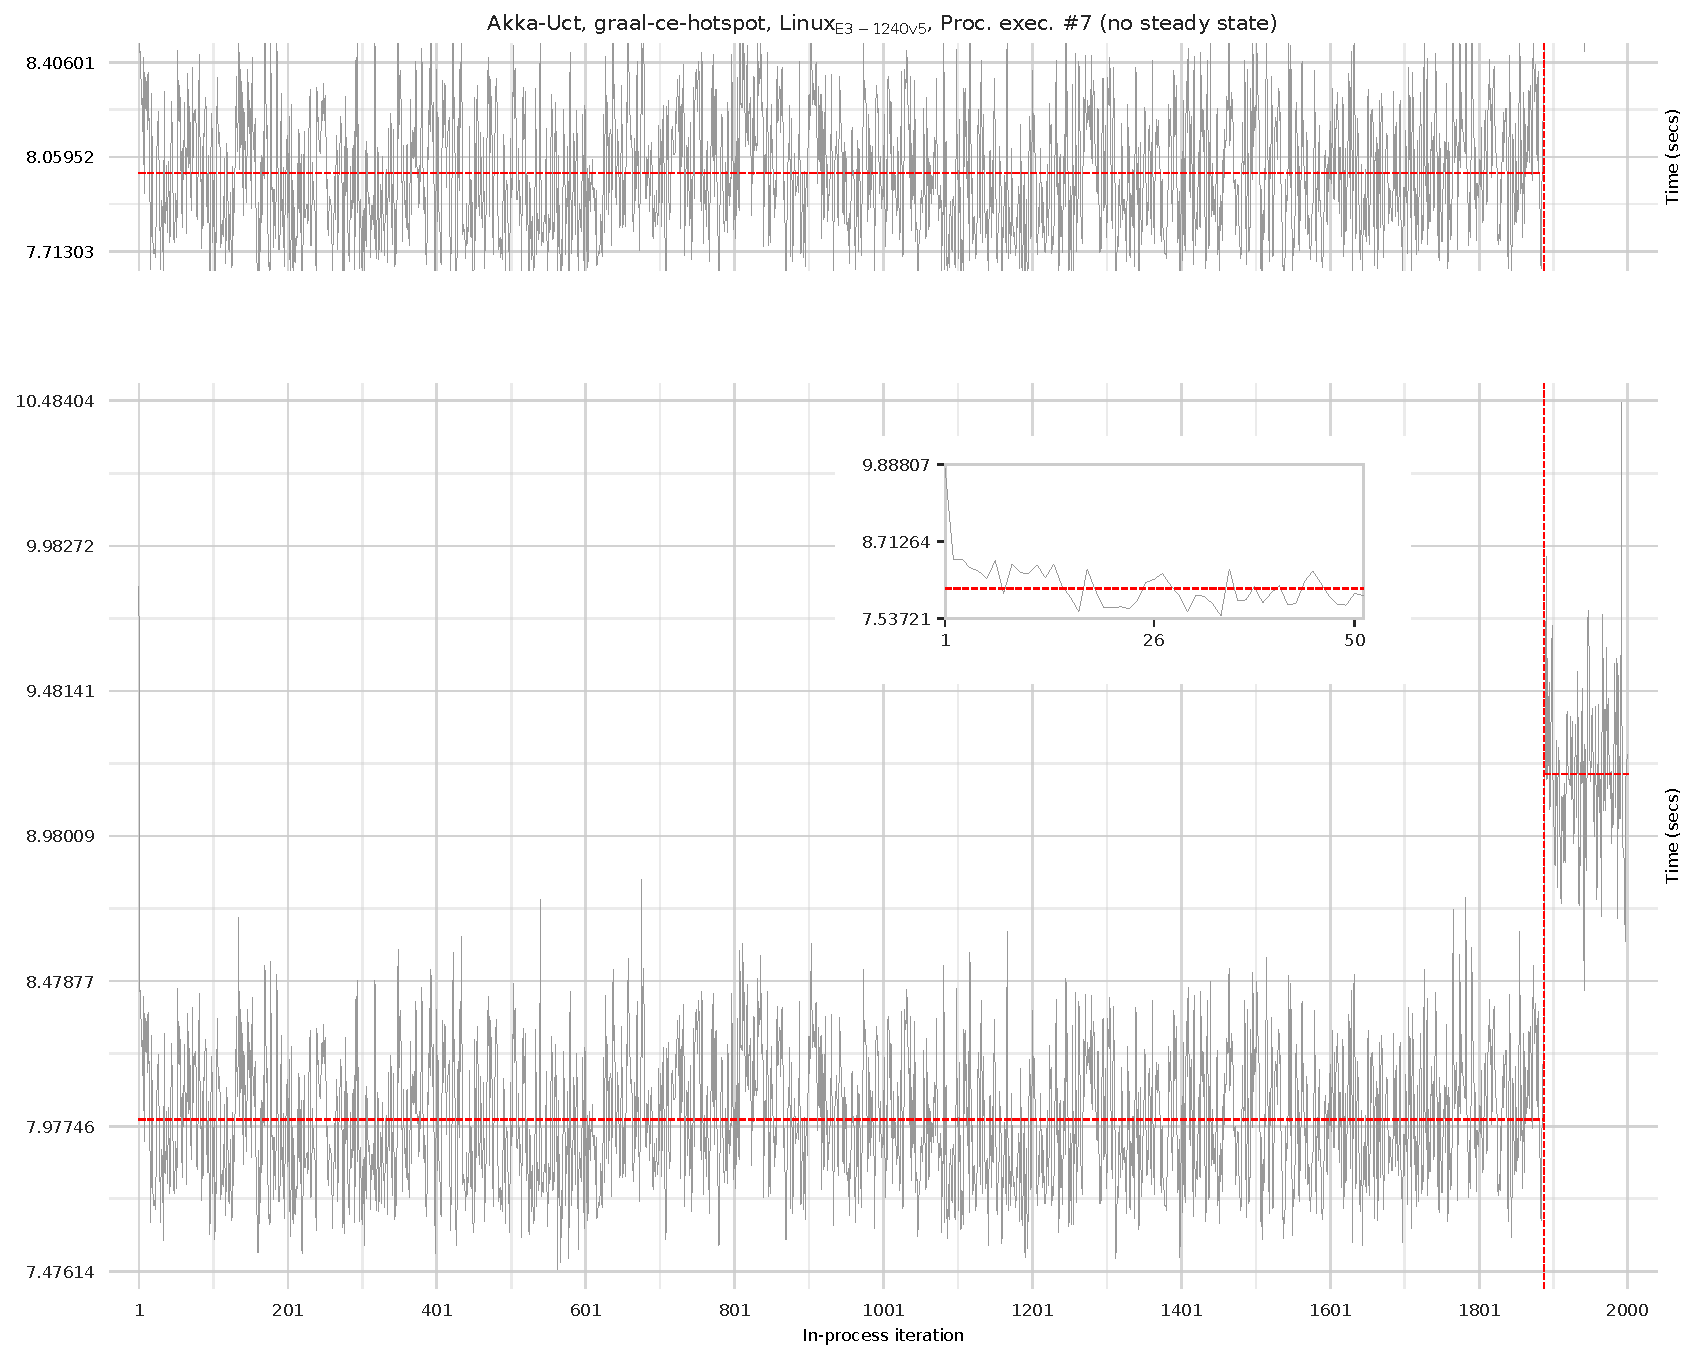
\includegraphics[width=.45\textwidth]{plots/slowdown1.pdf}
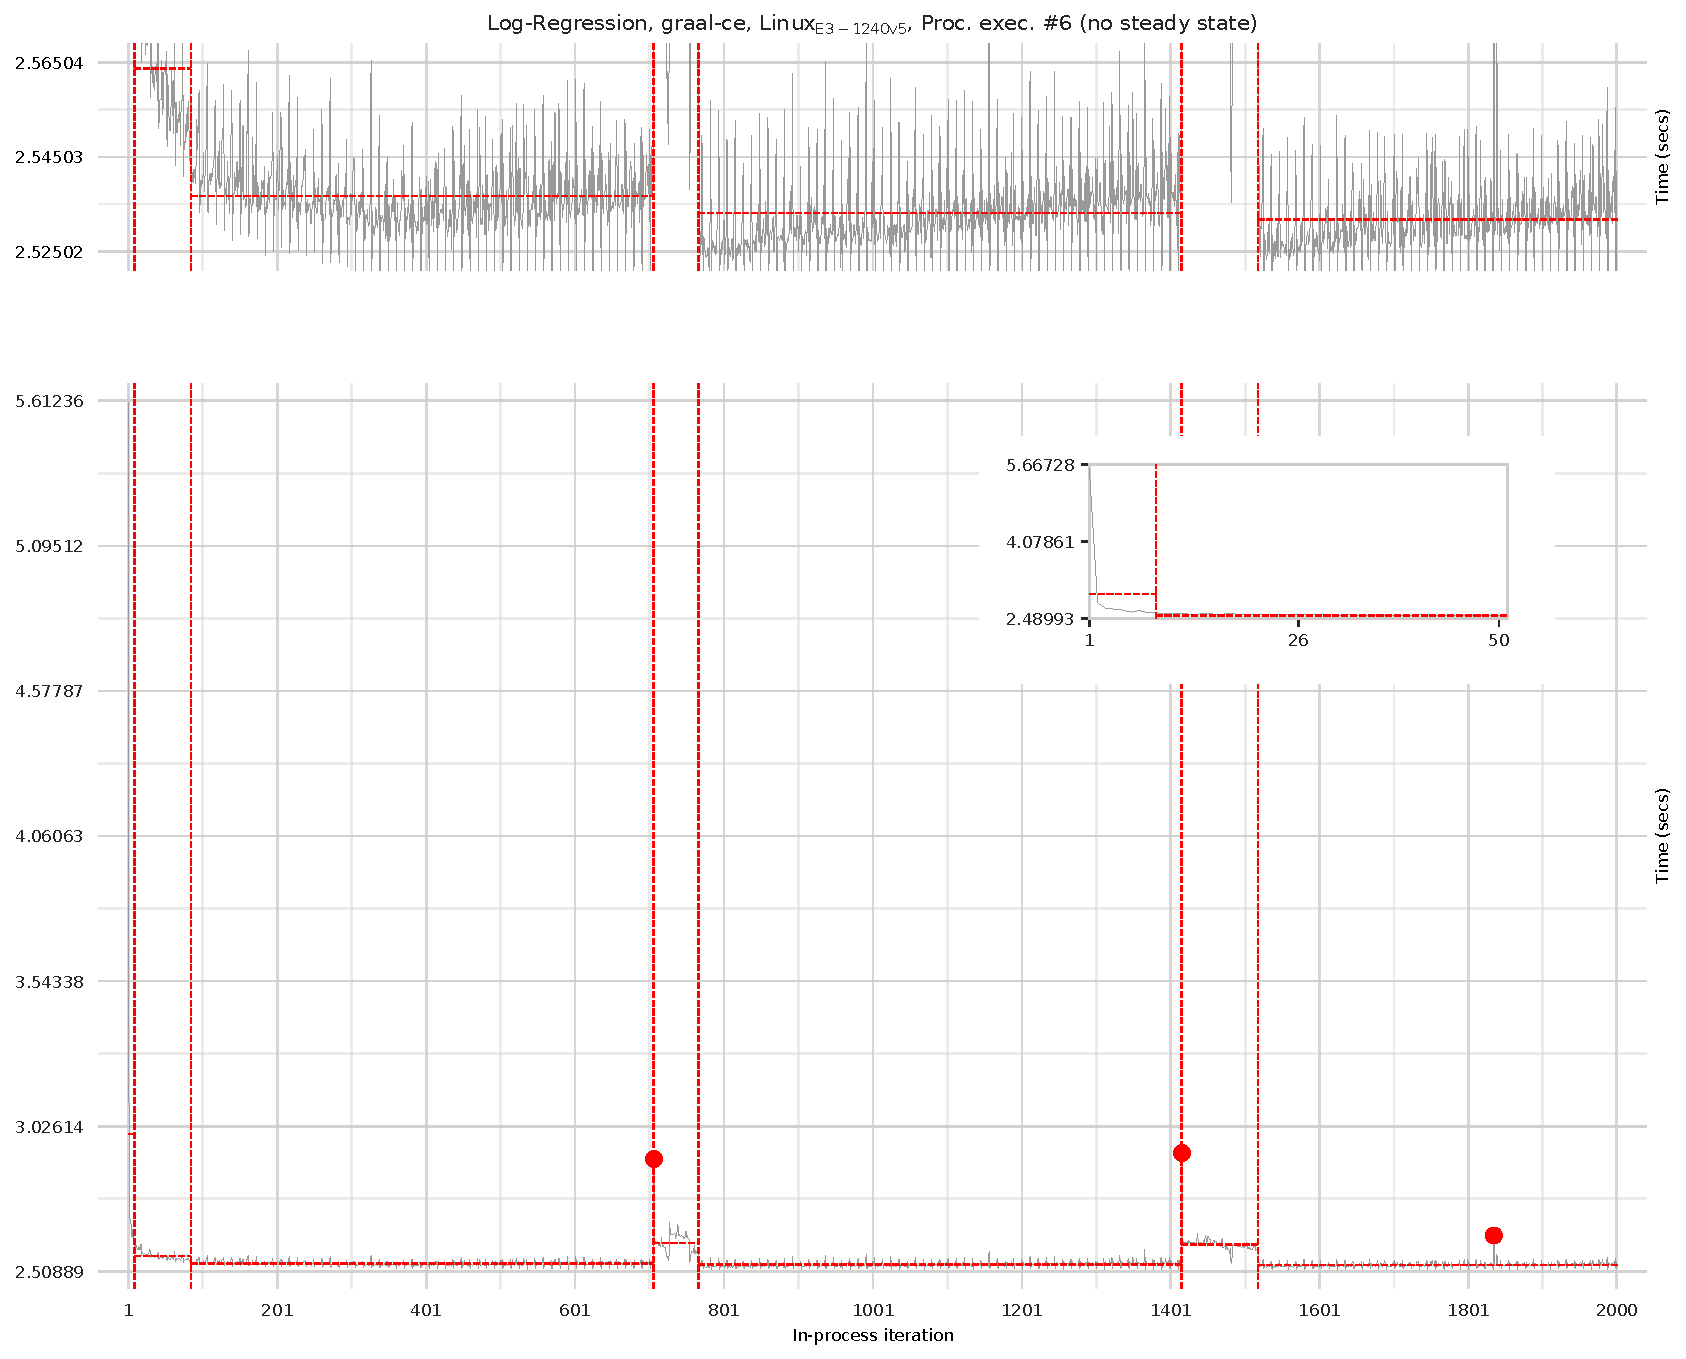
\includegraphics[width=.45\textwidth]{plots/no-steady1.pdf}\\
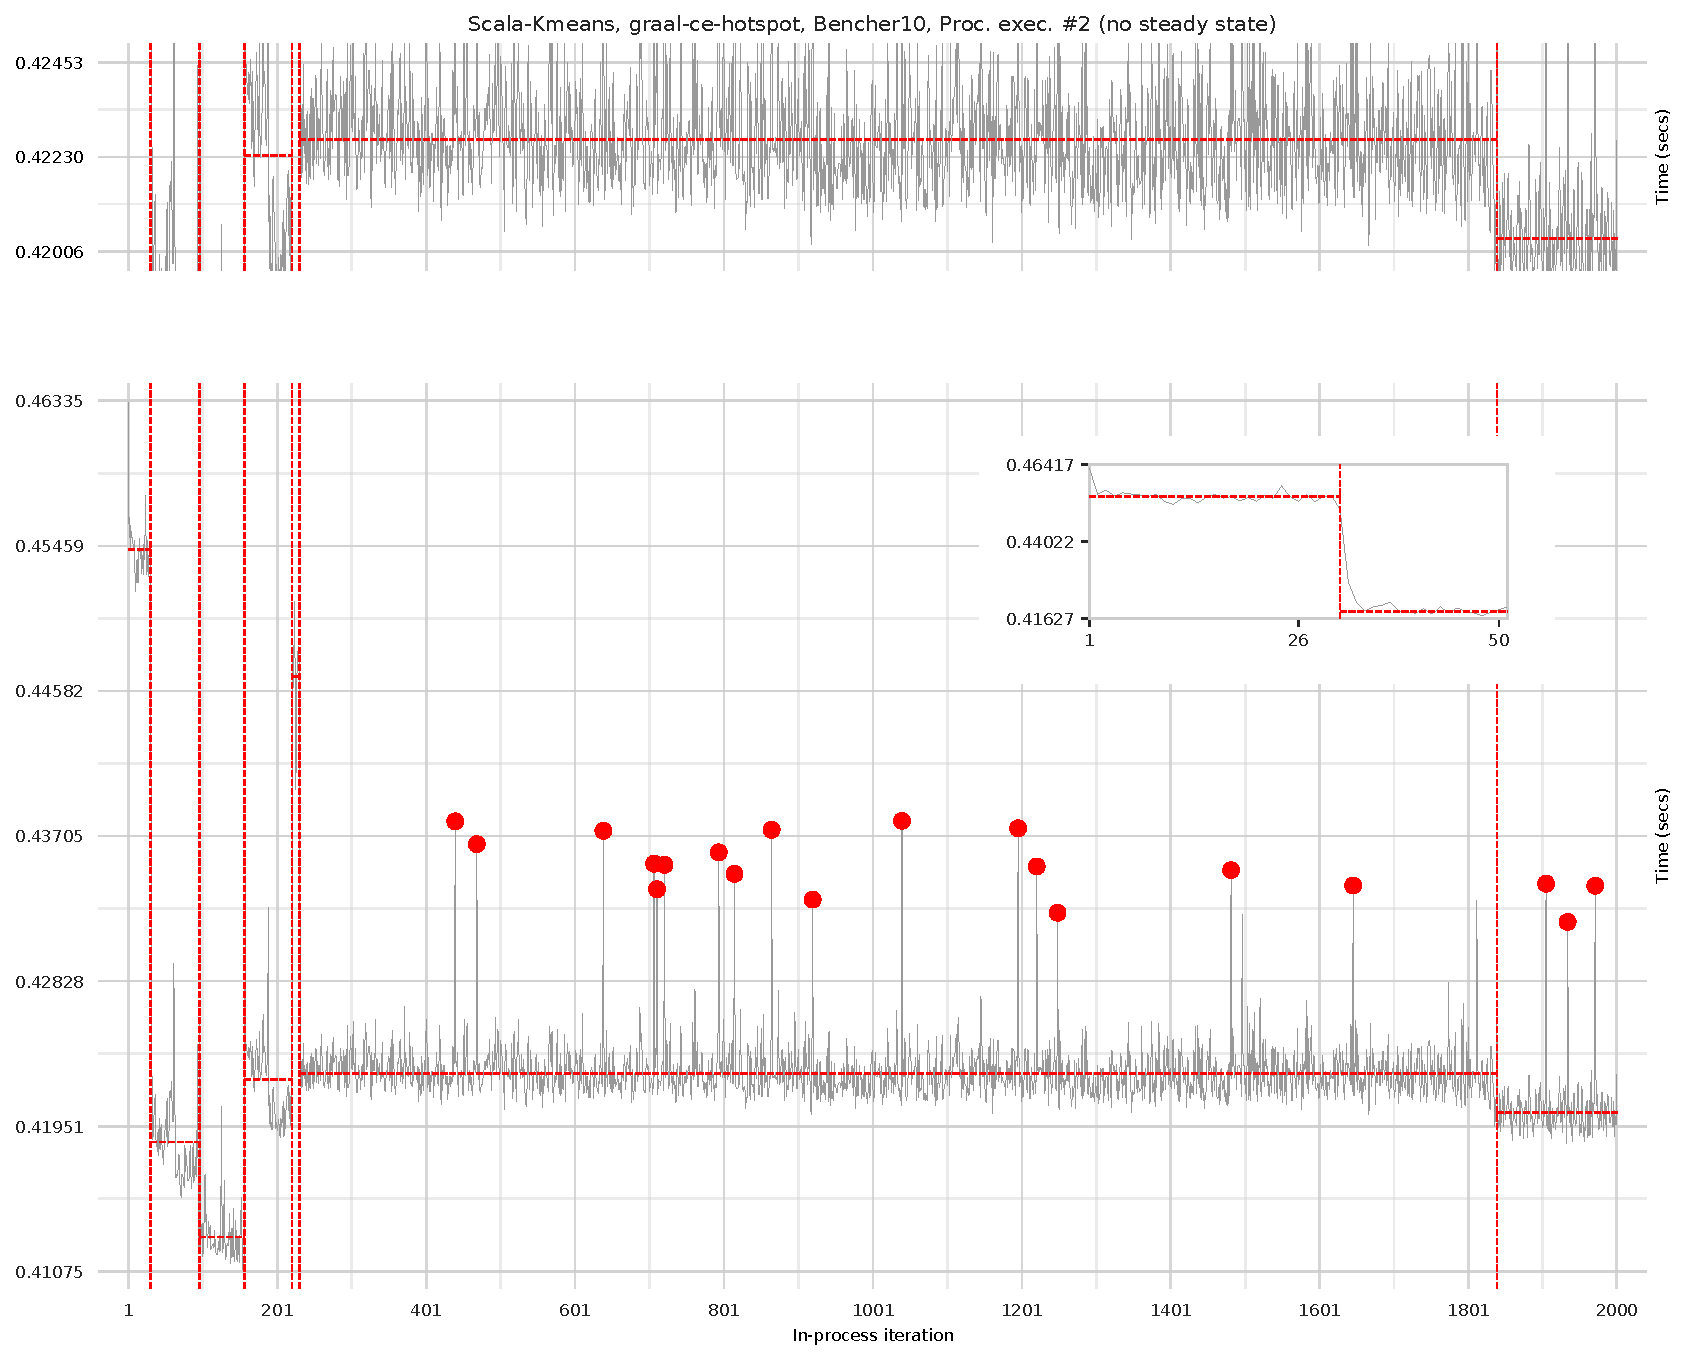
\includegraphics[width=.45\textwidth]{plots/no-steady2.pdf}
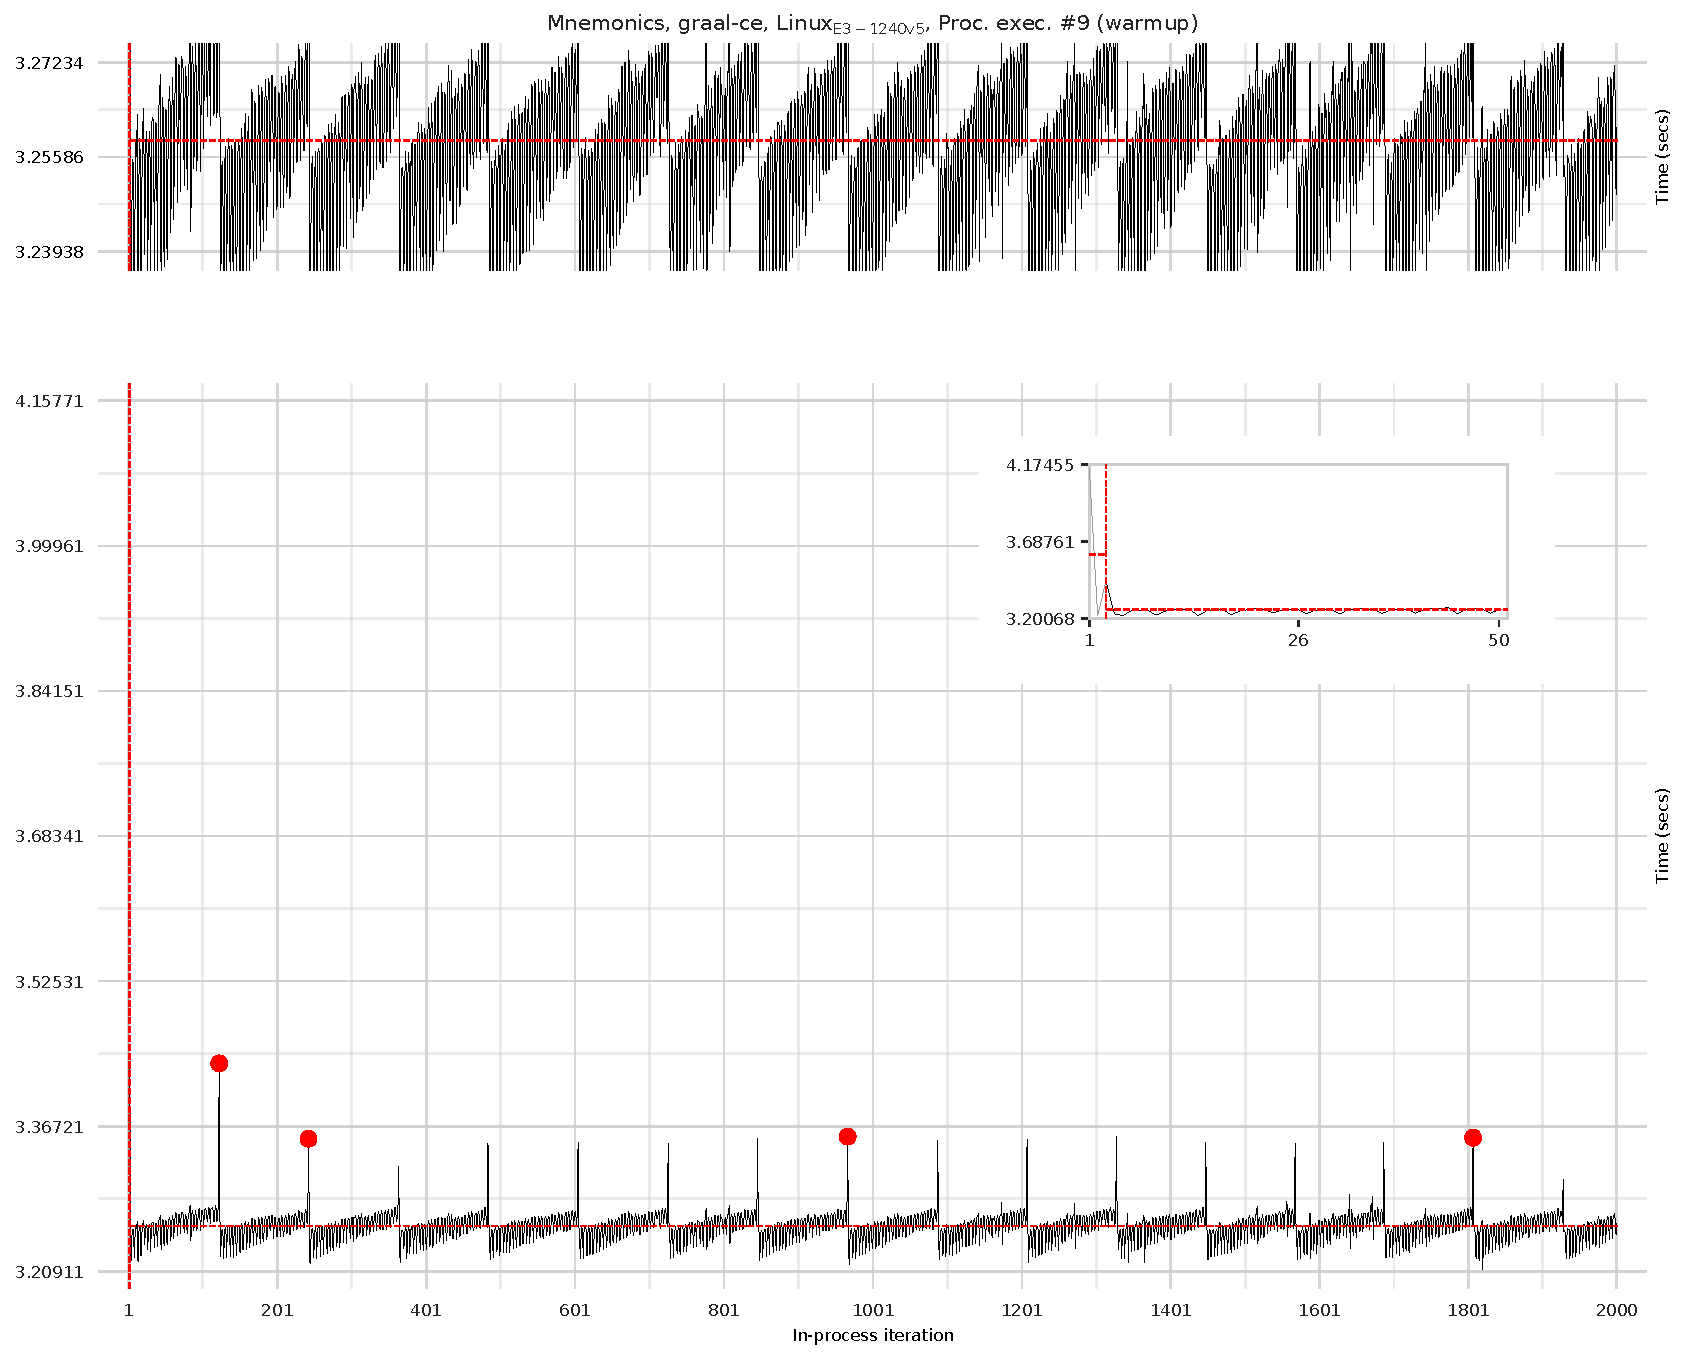
\includegraphics[width=.45\textwidth]{plots/cycles1.pdf}\\
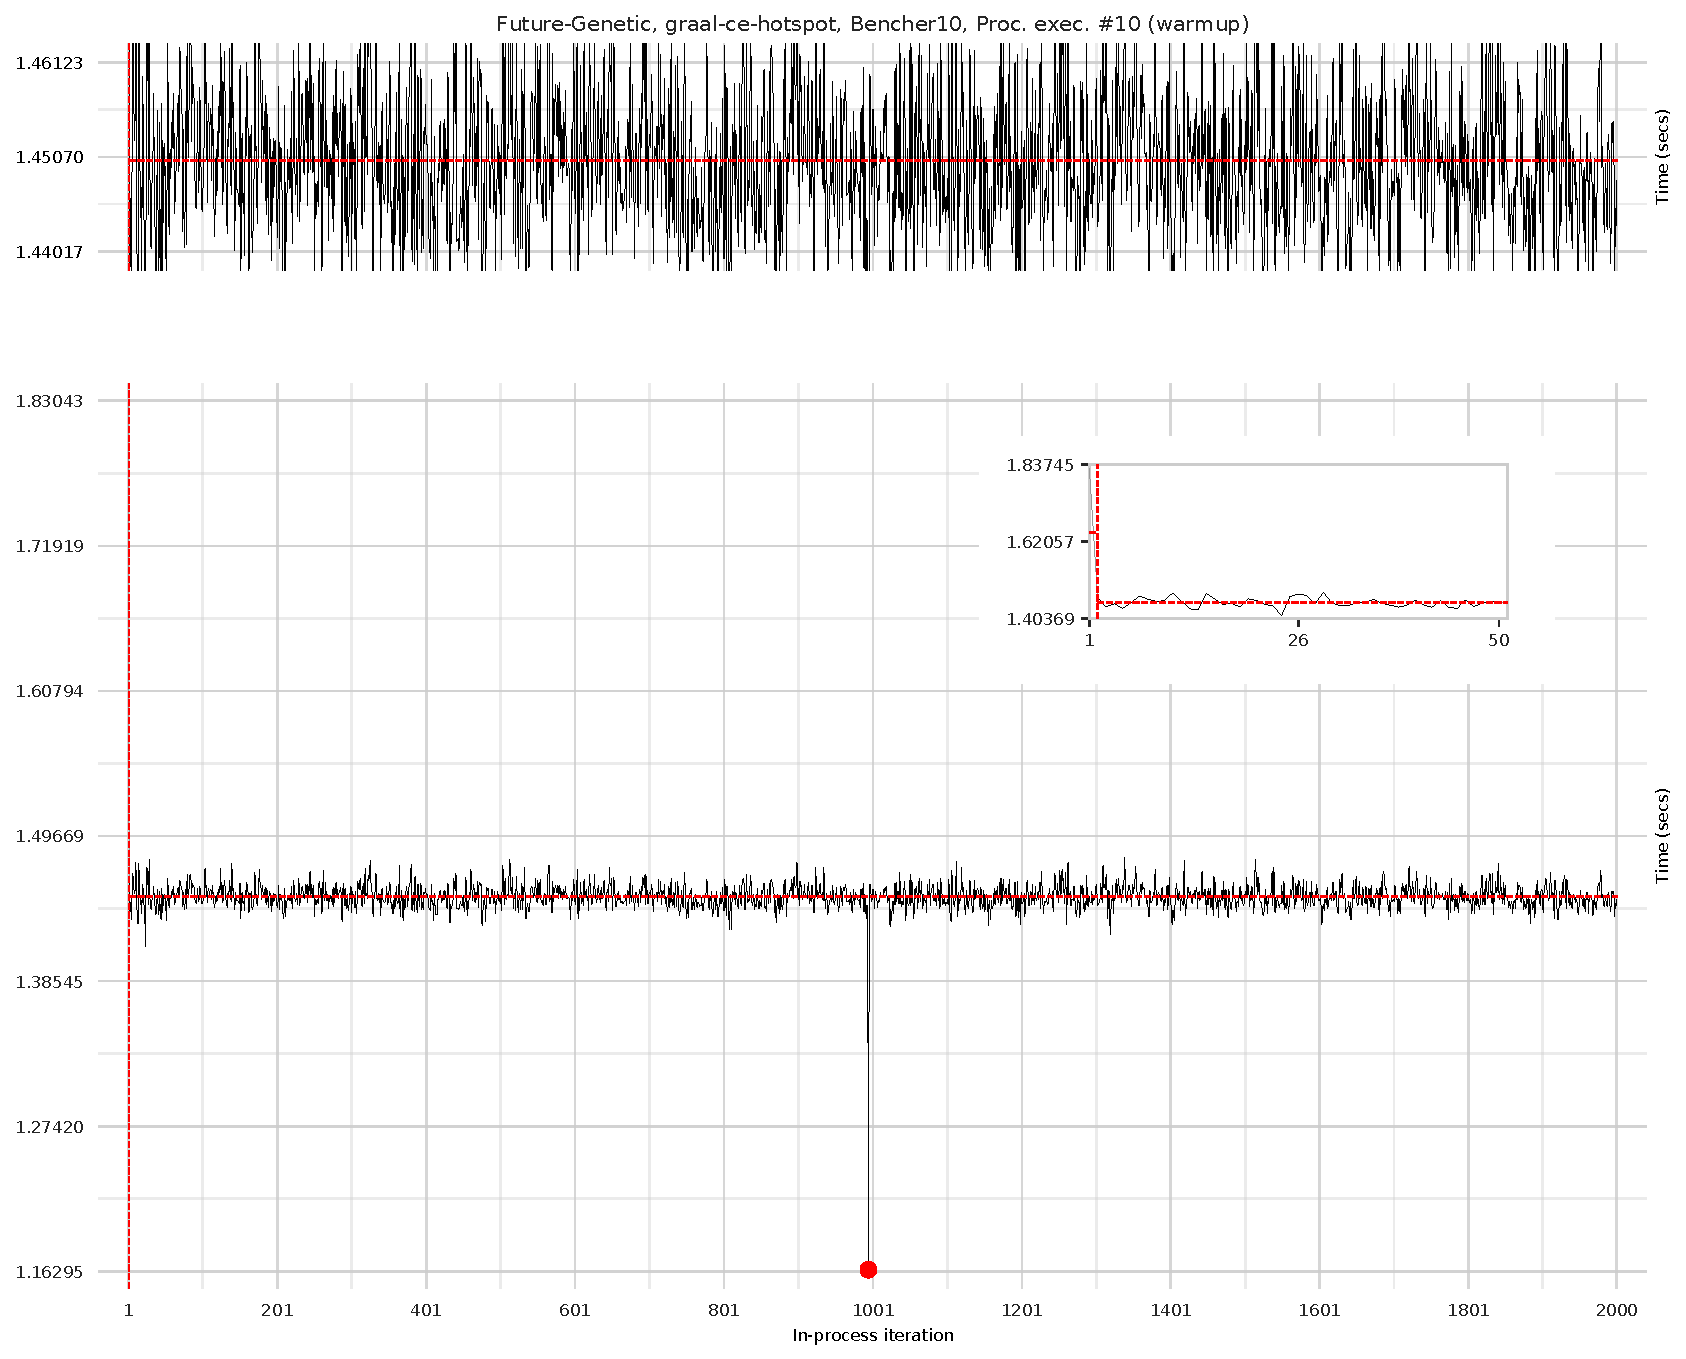
\includegraphics[width=.45\textwidth]{plots/outliers1.pdf}
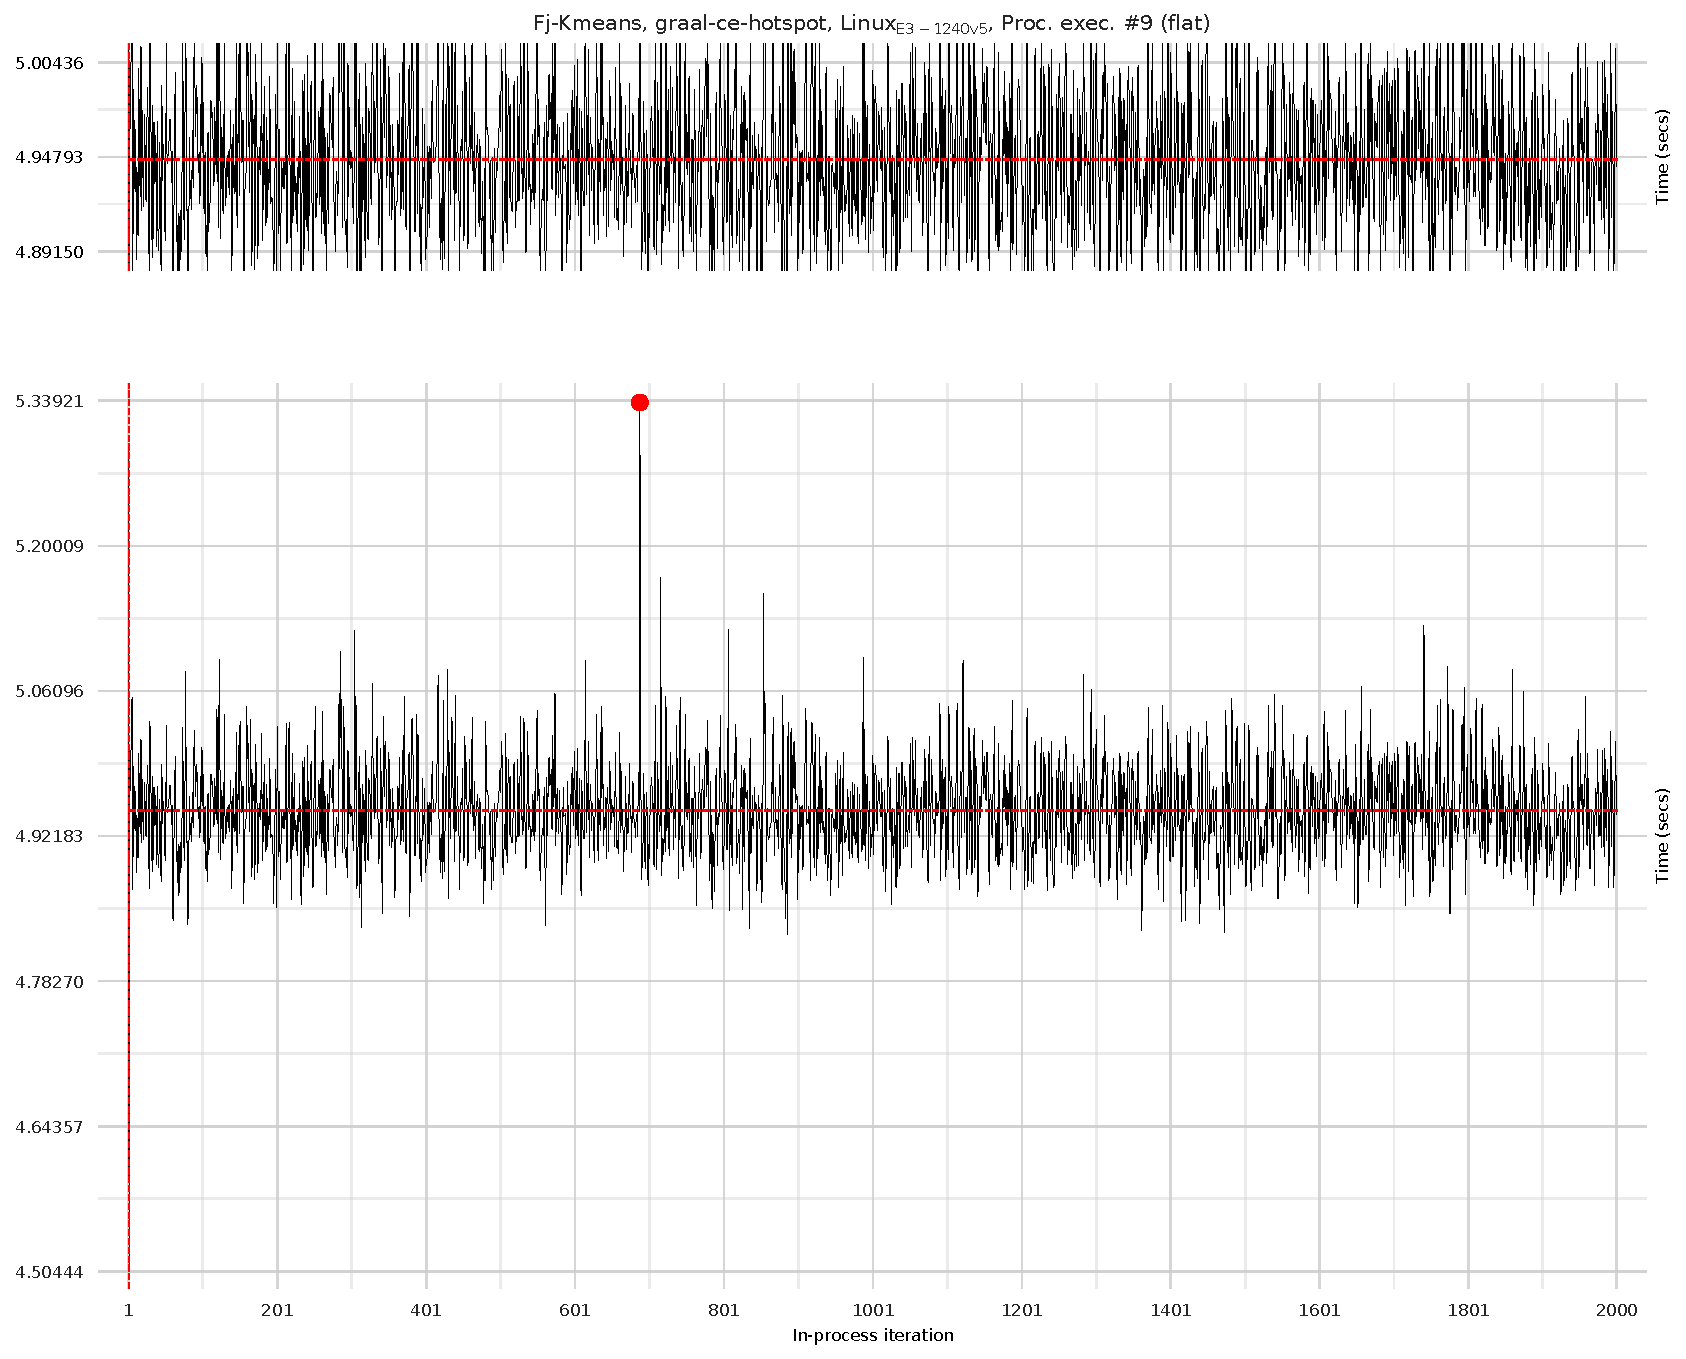
\includegraphics[width=.45\textwidth]{plots/fastearly1.pdf}\\
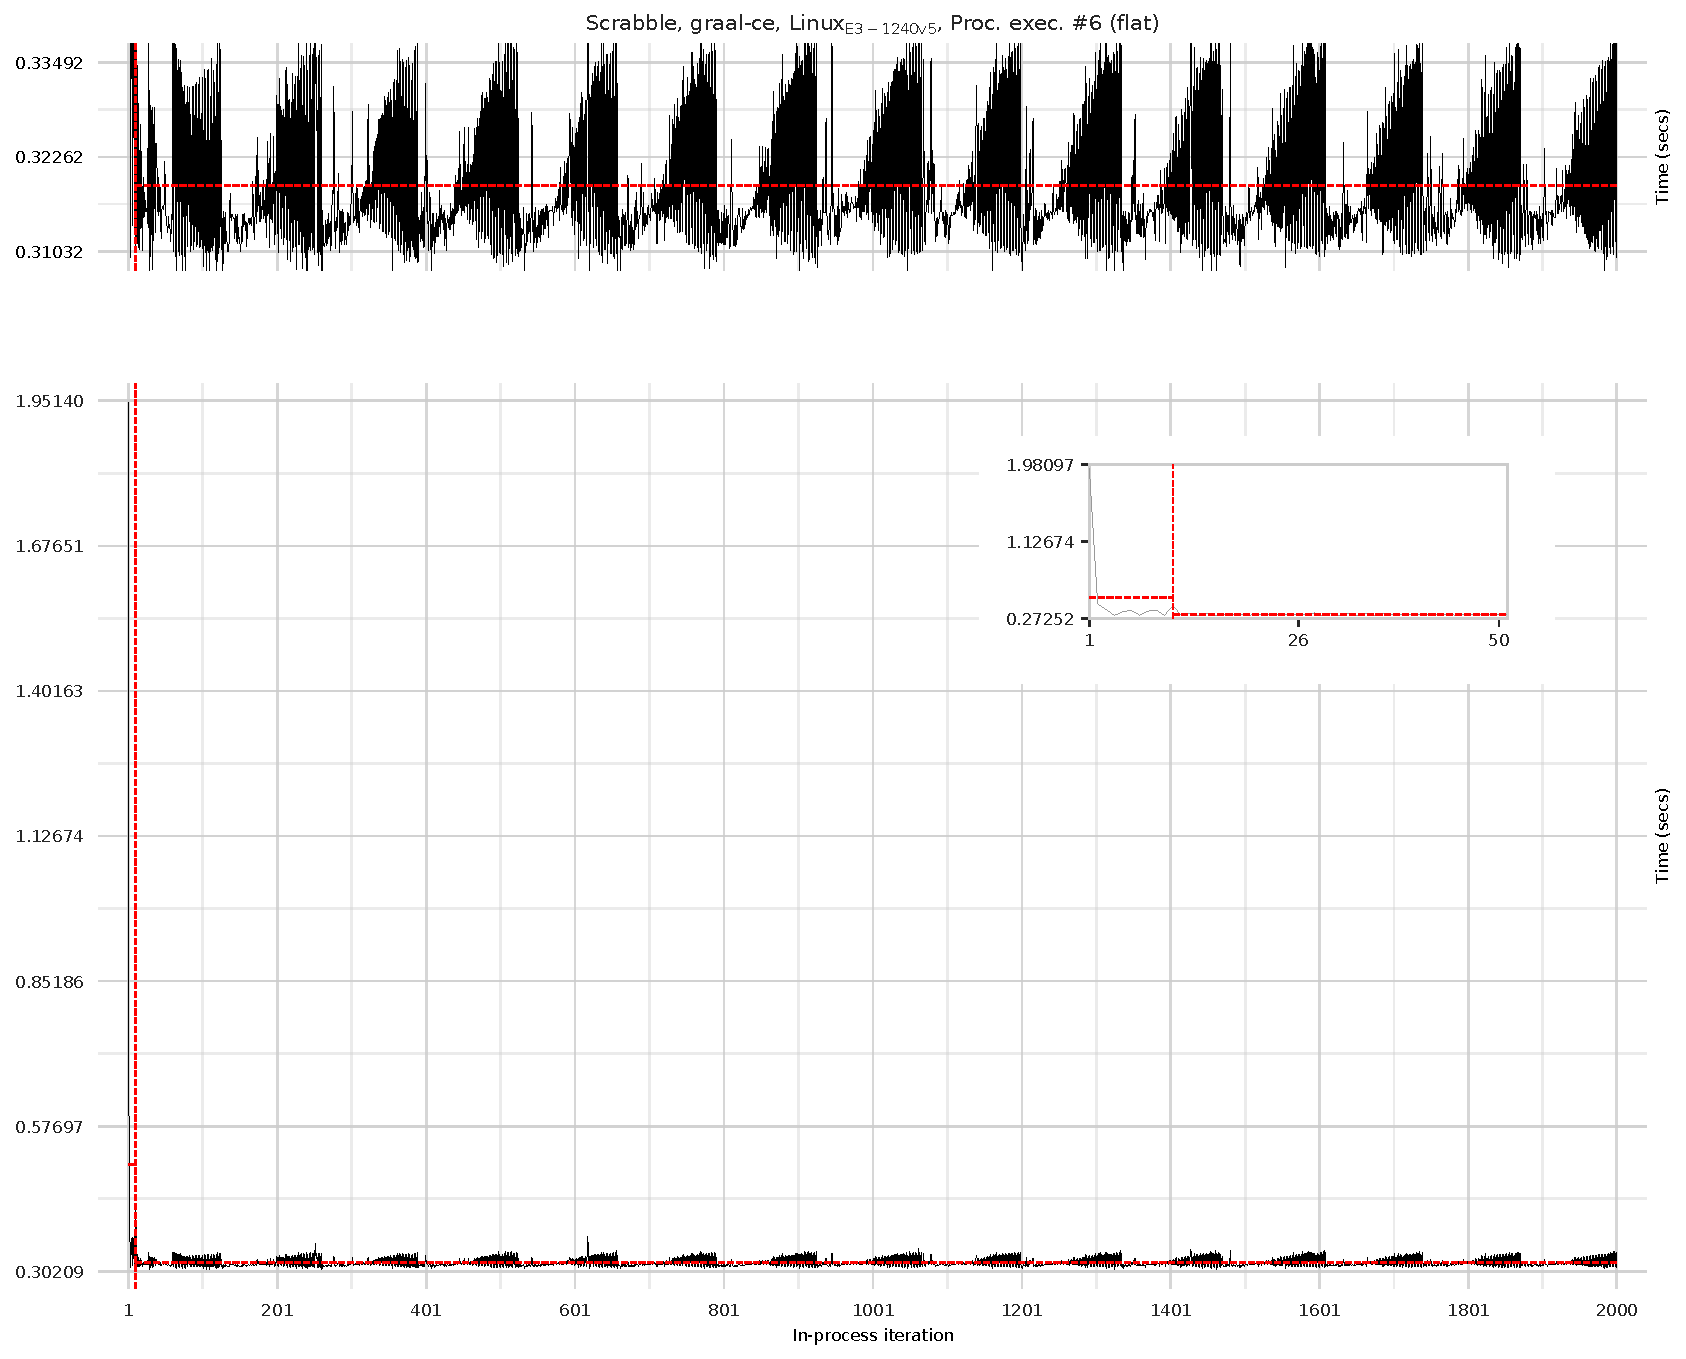
\includegraphics[width=.45\textwidth]{plots/steps1.pdf}

\end{document}
